%&fduthesis
\PassOptionsToPackage{OT1}{fontenc}
\PassOptionsToPackage{amsmath, thmmarks}{ntheorem}
\RequirePackage{
  amsmath,
  ctexhook,
  ctexpatch,
  fancyhdr,
  fix-cm,
  fontenc,
  graphicx,
  hyperref,
  ifvtex,
  l3keys2e,
  ntheorem,
  tikz,
  xcolor,
  xparse,
  xtemplate,
  zhnumber,
}
\let\maketitle\undefined

% tikz
\usetikzlibrary{arrows.meta, decorations.markings}
\tikzset{
  ->-/.style = {
    decoration = {
      markings,
      mark = at position #1 with {\arrow{Stealth}},
    },
    postaction = {decorate},
  },
}

\endofdump

\documentclass[type=doctor,oneside]{fduthesis}

\usepackage{enumitem}
\usepackage{tikz}

% fduthesis
\fdusetup{
  style = {
    font = libertinus,
    cjk-font = founder,
    fullwidth-stop = mapping,
    bib-backend = bibtex,
    bib-resource = {main.bib},
  },
  info = {
    title = {论文标题},
    title* = {Thesis Title},
    author = {曾祥东},
    supervisor = {孔令欣\quad 教授},
    major = {理论物理},
    degree = academic,
    department = {物理学系},
    student-id = {18110190010},
    % date = {2023 年 1 月 1 日},
    keywords = {不确定关系, 量子力学, 理论物理},
    keywords* = {Uncertainty principle, quantum mechanics, theoretical physics},
    clc = {O413.1},
  }
}

% enumitem
\setlist{itemsep=0pt}

% tikz
\usetikzlibrary{arrows.meta, decorations.markings}
\tikzset{
  ->-/.style = {
    decoration = {
      markings,
      mark = at position #1 with {\arrow{Stealth}},
    },
    postaction = {decorate},
  },
}

% Hacks
\ExplSyntaxOn
\__fdu_patch_cmd:Nnn \__fdu_load_cjk_font_founder:
  { \__fdu_setCJKmainfont:n  { FZShuSong-Z01 } }
  { \__fdu_setCJKmainfont:nn { FZShuSong-Z01 } { BoldFont = FZXiaoBiaoSong-B05 } }
\def\hypersetup{\kvsetkeys{Hyp}}
\ExplSyntaxOff

\AtBeginDocument{
  \setlength{\bibsep}{4pt plus 2pt minus 1pt}
}

% Math commands
\newcommand{\id}{\mathrm{id}}
\newcommand{\1}{\mathbf{1}}
\newcommand{\ldual}[1]{{}^\vee\mspace{-2mu}#1}
\DeclareMathOperator{\Hom}{Hom}
\DeclareMathOperator{\End}{End}
\DeclareMathOperator{\tr}{tr}

\newcommand{\tikzinput}[1]{\input{includes/tikz/#1.tex}}

\begin{document}

\frontmatter

\tableofcontents
\listoffigures

\begin{abstract}
  中文摘要
\end{abstract}

\begin{abstract*}
  English abstract
\end{abstract*}

\mainmatter

\chapter{张量融合范畴与弦网模型}

\section{范畴论基础}

\emph{范畴论} (category theory)\cite{baez2011physics,maclane2013categories,beer2018categories} 用以抽象地刻画一些数学结构之间的关系,它主要描述了“对象”之间的作用,即\emph{映射} (mapping)。拓扑序理论中所研究的,正是带有了某些附加结构的范畴。

一个\emph{范畴} $\mathcal{C}$ 由其中的\emph{对象} (object) $x\in\mathcal{C}$ 和这些对象之间的\emph{态射} (morphism) $f\colon x\to y$ 组成。对象之间的态射满足以下三个条件:
\begin{itemize}
  \item \emph{复合性} (composition):对于范畴 $\mathcal{C}$ 中的对象 $x$、$y$、$z$,若 $f\colon x\to y$ 和 $g\colon y\to z$ 为态射,则存在复合态射 $g\circ f\colon x\to z$;
  \item \emph{结合律} (associativity):若 $\mathcal{C}$ 中有态射 $f\colon x\to y$、$g\colon y\to z$、$h\colon z\to w$,则有
    \begin{equation}
      (h\circ g)\circ f = h\circ (g\circ f);
    \end{equation}
  \item \emph{单位元} (identity):对于 $\forall x\in\mathcal{C}$,都存在恒等态射 $\id_x\colon x\to x$,使得
    \begin{equation}
      f \circ \id_x = \id_x \circ f = f, \quad \forall f\colon x\to y.
    \end{equation}
\end{itemize}
态射也可记为 $f\in\Hom_{\mathcal{C}}(x,y)$,其中 $\Hom_{\mathcal{C}}(x,y)$ 称为同态集 (hom-set)。如果 $x=y$,则称 $f$ 为\emph{自同态} (endomorphism),记为 $f\in\End_{\mathcal{C}}(x)$。

\emph{函子} (functor) 是范畴之间保结构的映射。具体而言,对于范畴 $\mathcal{C}$、$\mathcal{D}$,函子 $F\colon\mathcal{C}\to\mathcal{D}$ 会将 $\mathcal{C}$ 中的对象 $x$ 映射到 $\mathcal{D}$ 中的对象 $F(x)$,而将 $\mathcal{C}$ 中的态射 $f\colon x\to y$ 映射到 $\mathcal{D}$ 中的态射 $F_f\colon F(x)\to F(y)$,并且保持复合性与单位元的成立,即
\begin{align}
  F_{\id_x} &= \id_{F(x)} \colon F(x) \to F(x), \quad \forall x\in\mathcal{C}, \\
  F_{g\circ f} &= F_g \circ F_f \colon F(x) \to F(z), \quad \forall f\colon x\to y, \, g\colon y\to z.
\end{align}

在函子之上可进一步定义\emph{自然变换} (natural transformation)。对于两个函子 $F\colon\mathcal{C}\to\mathcal{D}$ 和 $G\colon\mathcal{C}\to\mathcal{D}$,自然变换 $\tau\colon F\Rightarrow G$ 由其分量 $\tau_x$(这是范畴 $\mathcal{D}$ 中的一个态射)定义:
\begin{equation}
  \tau_x\colon F(x)\to G(x), \quad \forall x\in\mathcal{C},
\end{equation}
它满足
\begin{equation}
  \tau_y \circ F_f = G_f \circ \tau_x, \quad \forall f\colon x\to y.
\end{equation}
如图~\ref{fig:natural-transformation},自然变换可以用交换图来直观地表示。若 $\tau$ 的每一分量 $\tau_x$ 均可逆(即存在 $\tau_x^{-1}$ 使得 $\tau^{-1}_x\circ\tau_x=\id_{F(x)}$ 且 $\tau_x\circ\tau^{-1}_x = \id_{G(x)}$),则称其为\emph{自然同构} (natural isomorphism),我们用 $\similarrightarrow$ 来表示。

\begin{figure}[htb]
  \centering
  \begin{tabular}{c@{\qquad}c}
    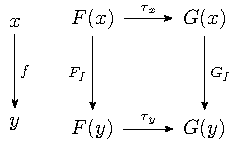
\includegraphics{images/natural-transformation-1.pdf} &
    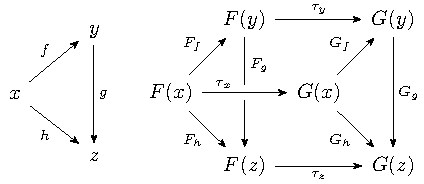
\includegraphics{images/natural-transformation-2.pdf} \\
    (a) & (b)
  \end{tabular}
  \caption[自然变换对应的交换图]{自然变换对应的交换图。(a) 此图是“可交换的”,即从 $F(x)$ 到 $G(y)$ 的两条路径等价;(b) 对于结合律的“提升”,图中三棱柱的三个侧面都是可交换的。}
  \label{fig:natural-transformation}
\end{figure}

\begin{example}
  对于任意的交换环 $K$,以其中元素构成的 $n\times n$ 的非奇异矩阵组成了一般线性群 $GL_n(K)$。对于环同态 $f\colon K\to L$,显然可以构建群同态 $GL_n f\colon GL_n(K)\to GL_n(L)$。因此,$GL_n$ 即为交换环范畴 $\mathbf{CRng}$ 到群范畴 $\mathbf{Grp}$ 的函子。

  设非奇异矩阵 $M\in GL_n(K)$,则其行列式 $\det_K(M)$ 为 $K$ 中的可逆元(即单位),因而 $\det_K$ 是群同态 $GL_n(K)\to K^\times$,其中 $K^\times$ 为 $K$ 的可逆元群。另一方面,当把环同态 $f$ 限制在可逆元群上时,可得群同态 $f^\times\colon K^\times\to L^\times$,因而 $(\cdot)^\times$ 同样也是 $\mathbf{CRng}$ 到 $\mathbf{Grp}$ 的函子。根据定义,$\det\colon GL_n\Rightarrow(\cdot)^\times$ 即为自然变换,它满足 $\det_L\circ\,GL_n f=f^\times\circ \det_K$。
\end{example}

% \begin{example}
%   在 Haskell 编程语言中,类型为范畴 $\mathbf{Hask}$ 中的对象,而纯函数为态射。函子可由类型类 (type class) 来定义,例如 \verb|List| 可以将类型 \verb|T| 构造为对应的数组 \verb|[T]|,并且通过 \verb|fmap| 将以 \verb|T| 类型为参数的纯函数转换为以 \verb|[T]| 类型为参数的纯函数。自然变换则由参数多态 (parametric polymorphism) 实现。例如,一个安全的(不引发异常)返回数组首元素的函数可按下面的方式定义:
% \begin{verbatim}
%   head :: [T] -> Maybe T
%   head []     = Nothing
%   head (x:xs) = Just x
% \end{verbatim}
%   因此 \verb|head| 函数是从 \verb|List| 到 \verb|Maybe| 的自然变换。
% \end{example}

\emph{弦图} (string diagram) 可以更直观地描述范畴的概念。其中,带箭头的直线或曲线代表对象,盒子代表态射\cite{selinger2011survey,baez2011physics}:
\begin{equation}
  f\colon x\to y \quad \coloneq \quad
  \tikzinput{morphism} \, .
\end{equation}
这样态射的复合就可以表示为连在一起的两个盒子:
\begin{equation}
  \tikzinput{composition}.
\end{equation}

\section{张量范畴与融合范畴}
\label{sec:tensor-category-fusion-category}

\subsection{张量范畴}

我们可以在范畴中引入一些结构,使其具有新的特性。引入了张量积的范畴为\emph{张量范畴} (tensor category)\cite{bakalov2001lectures,muger2008tensor,maclane2013categories,beer2018categories,kong2022invitation}。它最基本也最重要的例子是向量空间(或对应的范畴 $\mathbf{Vec}$),其中的张量积结构即为两个向量空间和相应线性变换的直积。一个张量范畴 $\mathcal{C}$ 由下面的条件定义:
\begin{itemize}
  \item \emph{张量积} (tensor product) $\otimes\colon\mathcal{C}\times\mathcal{C}\to\mathcal{C}$ 和\emph{单位对象} (unit object) $\1\in\mathcal{C}$;
  \item \emph{结合子} (associator) $\alpha$,它是一个自然同构:
    \begin{equation}
      \alpha_{x,y,z} \colon (x\otimes y)\otimes z \similarrightarrow x\otimes(y\otimes z), \quad \forall x,y,z \in \mathcal{C};
    \end{equation}
  \item \emph{左右单位子} (left/right unitor),同样也是自然同构:
    \begin{equation}
      \lambda_x \colon \1\otimes x \similarrightarrow x, \quad
      \rho_x    \colon x\otimes\1  \similarrightarrow x, \quad
      \forall x \in \mathcal{C}.
    \end{equation}
\end{itemize}
它们需要满足五边形方程和三角形方程(图~\ref{fig:pentagon-triangle-equation})。

\begin{figure}[htb]
  \centering
  \begin{tabular}{cc}
    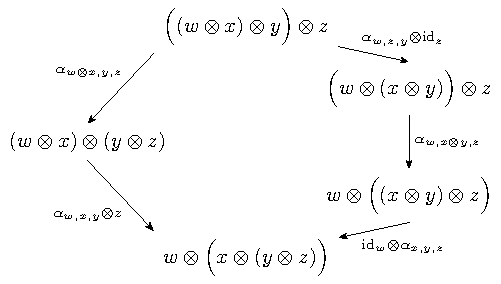
\includegraphics{images/pentagon-equation.pdf} &
    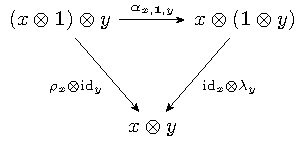
\includegraphics{images/triangle-equation.pdf} \\
    (a) & (b)
  \end{tabular}
  \caption[五边形方程和三角形方程对应的交换图]{五边形方程 (a) 和三角形方程 (b) 对应的交换图。}
  \label{fig:pentagon-triangle-equation}
\end{figure}

如果上述定义中的 $\similarrightarrow$ 可以取为等号,则称该张量范畴是\emph{严格} (strict) 的,此时 $\alpha$、$\lambda$ 和 $\rho$ 均为恒等变换。根据 MacLane \emph{一致性定理} (coherence theorem),每个张量范畴都等价于一个严格张量范畴\cite{maclane2013categories}。因此我们之后可以只考虑严格张量范畴的情况。此时张量积表达式中的括号和单位对象都可以忽略。

一个张量范畴也是一个\emph{幺半群} (monoid),因为范畴的单位对象可以作为群的单位元,而张量积可以作为群乘法。所以张量范畴也被称为\emph{幺半范畴} (monoidal category)。

\subsection{对偶}

类似于对偶空间的概念,我们可以在张量范畴中引入\emph{对偶} (dual) 的概念。$x\in\mathcal{C}$ 的\emph{右对偶} (right dual) $x^\vee$ 通过以下两个态射定义:
\begin{equation}
  e_x\colon x^\vee\otimes x\to\1, \quad i_x\colon\1\to x\otimes x^\vee,
\end{equation}
它们需要满足\emph{刚性公理} (rigidity axioms):
\begin{equation}
  \begin{aligned}
    (\id_x\otimes e_x) \circ (i_x\otimes\id_x) &= \id_x, \\
    (e_x\otimes\id_{x^\vee}) \circ (\id_{x^\vee}\otimes i_x) &= \id_{x^\vee}.
  \end{aligned}
\end{equation}
如果在弦图中省略单位元(对应于物理中的真空态),则 $e_x$ 和 $i_x$ 可以表示为
\begin{equation}
  \tikzinput{dual-1},
  \qquad
  \tikzinput{dual-2}.
\end{equation}
这可以类比于量子力学中的湮灭与产生算符。(右对偶的)刚性公理则可表示为
\begin{equation}
  \tikzinput{rigidity-axioms-1},
  \qquad
  \tikzinput{rigidity-axioms-2}.
  \label{eq:rigidity-axioms-diagrams}
\end{equation}

同理,我们还可以定义\emph{左对偶} (left dual):
\begin{equation}
  e'_x \colon x\otimes \ldual{x}\to\1, \quad i'_x\colon \1\to\ldual{x}\otimes x.
  \label{eq:left-dual}
\end{equation}
这实际上只需要对上面的图沿水平方向做一下镜像操作。如果 $\mathcal{C}$ 中的每个对象既有左对偶也有右对偶,则称其为是\emph{刚性} (rigid) 的或\emph{自治} (autonomous) 的;而如果 $\forall x\in\mathcal{C}$,都有 $x=x^\vee$,则称 $\mathcal{C}$ 是\emph{自对偶} (self-dual) 的。

\subsection{中枢与球状结构}

我们知道有限维向量空间 $V$ 的二重对偶 $V^{\vee\vee}$ 同构于 $V$。这在张量范畴中的推广即为\emph{中枢} (pivotal) 结构,它是由以下的自然同构给出的:
\begin{equation}
  \delta_x \colon x \similarrightarrow x^{\vee\vee}, \quad \forall x\in\mathcal{C},
\end{equation}
且需满足
\begin{equation}
  \delta_{x\otimes y} = \delta_x\otimes\delta_y, \quad
  \delta_{\1} = \id_{\1}, \quad
  \delta_{x^\vee} = (\delta_x^\vee)^{-1}.
\end{equation}
根据右对偶的定义,可有
\begin{equation}
  e_x\colon x^\vee\otimes x \similarrightarrow x^\vee\otimes x^{\vee\vee}\to\1, \quad
  i_x\colon \1\to x\otimes x^\vee \similarrightarrow x^{\vee\vee}\otimes x^\vee.
\end{equation}
对比式~\eqref{eq:left-dual},可以发现 $x^{\vee\vee}$ 也是 $x^\vee$ 的左对偶。若令 $y=x^\vee$,即有 $\ldual{y}=y^\vee$,也就是说在中枢范畴中可以不再区分左右对偶。

对于中枢范畴 $\mathcal{C}$ 中的自同态 $f\in\End_{\mathcal{C}}(x)$,可以定义\emph{左右迹} (left/right trace):
\begin{equation}
  \begin{aligned}
    \tr_{\text{L}} f &\colon \1
      \xrightarrow{i_{x^\vee}} x^\vee\otimes x^{\vee\vee}
      \xrightarrow{\id_{x^\vee}\otimes\delta_x^{-1}} x^\vee\otimes x
      \xrightarrow{\id_{x^\vee}\otimes f} x^\vee\otimes x
      \xrightarrow{e_x} \1, \\
    \tr_{\text{R}} f &\colon \1
      \xrightarrow{i_x} x\otimes x^\vee
      \xrightarrow{f\otimes\id_{x^\vee}} x\otimes x^\vee
      \xrightarrow{\delta_x\otimes\id_{x^\vee}} x^{\vee\vee}\otimes x^\vee
      \xrightarrow{e_{x^\vee}} \1.
  \end{aligned}
\end{equation}
当 $f=\id_x$ 时,还可以定义\emph{左右维数} (left/right dimension):
\begin{equation}
  \dim_{\text{L}} x \coloneq \tr_{\text{L}}\id_x, \quad
  \dim_{\text{R}} x \coloneq \tr_{\text{R}}\id_x.
  \label{eq:left-right-dimension}
\end{equation}
迹和维数可以用下图来描述:
\begin{equation}
  \tr_{\text{L}}  f = \tikzinput{trace-1} \, , \quad
  \tr_{\text{R}}  f = \tikzinput{trace-2} \, ; \quad
  \dim_{\text{L}} x = \tikzinput{dimension-1} \!, \quad
  \dim_{\text{R}} x = \tikzinput{dimension-2} \!.
\end{equation}
如果对于任意的 $f\in\End_{\mathcal{C}}(x)$ 都有 $\tr_{\text{L}}f=\tr_{\text{R}}f$,则称 $\mathcal{C}$ 是\emph{球状} (spherical) 的。

\subsection{融合范畴}

范畴中还可以引入\emph{直和} (direct sum) 的结构。若范畴 $\mathcal{C}$ 中的对象均可分解为\emph{简单对象} (simple object) 的直和:
\begin{equation}
  x = \bigoplus_{i\in I} n_i x_i, \quad \forall x \in \mathcal{C},
\end{equation}
其中 $x_i\in\mathcal{C}$ 是简单对象,$I$ 是由非零简单对象(等价类)构成的指标集,而系数 $n_i\in\mathbb{Z}_+$,则称 $\mathcal{C}$ 是一个\emph{半单范畴} (semi-simple category)。简单对象的例子包括向量空间范畴 $\mathbf{Vec}$ 中的一维空间(直线),以及 Abel 群范畴 $\mathbf{Ab}$ 中的单群。

若张量范畴 $\mathcal{C}$ 同时也是半单的,并且简单对象只有有限多个,那么这样的 $\mathcal{C}$ 称为\emph{融合范畴} (fusion category)\cite{bakalov2001lectures,kitaev2006anyons,bruillard2016rank,aasen2020topological,lou2021dummy}。此时简单对象的张量积可以写成:
\begin{equation}
  x_a \otimes x_b = \bigoplus_c N_{ab}^c x_c,
\end{equation}
其中 $N_{ab}^c\in\mathbb{Z}_+$,称为\emph{融合系数} (fusion coefficient)。在物理学中一般可以假设 $N_{ab}^c$ 只能取到 0 或 1,即是否允许该融合发生。所有允许的融合称为\emph{融合规则} (fusion rule)。融合范畴还要与张量范畴的结构相容,这意味着
\begin{equation}
  N_{\1 a}^b = N_{a\1}^b = \delta_{ab}, \quad
  \sum_x N_{ax}^z N_{bc}^x = \sum_y N_{ab}^y N_{yc}^z.
\end{equation}
我们还要求融合范畴是刚性且自对偶的,此时可以证明
\begin{equation}
  N_{ab}^c = N_{ba}^c = N_{ac}^b = N_{ca}^b = N_{bc}^a = N_{cb}^a,
\end{equation}
即融合系数关于所有指标均对称。

定义矩阵 $(N_a)_{bc}\coloneq N_{ab}^c$,根据 Perron--Frobenius 定理,可知 $N_a$ 存在最大的非负特征值,这定义为简单对象 $a$ 的\emph{量子维数} (quantum dimension)或 Perron--Frobenius 维数 $d_a$。可以证明,量子维数与式~\eqref{eq:left-right-dimension} 中通过迹定义的维数是相同的。融合范畴 $\mathcal{C}$ 的\emph{总量子维数} (total quantum dimension) 定义为
\begin{equation}
  D = \sqrt{\sum_{i\in I} d_i^2}.
\end{equation}

融合的逆运算是\emph{分裂} (splitting)。简单对象的融合与分裂都可以用弦图来表示:
\begin{equation}
  \tikzinput{fusion-tree-1}
  \in \Hom_{\mathcal{C}}(a\otimes b, c) \eqcolon V^{ab}_c, \quad
  \tikzinput{fusion-tree-2}
  \in \Hom_{\mathcal{C}}(c, a\otimes b) \eqcolon V_{ab}^c.
\end{equation}
由于 $\mathcal{C}$ 的刚性和自对偶性,我们可以省略弦图中的箭头。此时,$\Hom_{\mathcal{C}}(a\otimes b,c)$ 和 $\Hom_{\mathcal{C}}(c,a\otimes b)$ 都是向量空间,分别记为 $V^{ab}_c$ 和 $V_{ab}^c$,上面的“融合树”正是对应的基向量。这两个向量空间的维数相等,都等于融合系数 $N_{ab}^c$。

下面我们考虑向量空间 $V^{abc}_d$,它表示从 $a\otimes b\otimes c$ 到 $d$ 的融合。由于 $\mathcal{C}$ 是严格的,$(a\otimes b)\otimes c$ 和 $a\otimes(b\otimes c)$ 的结果相同(都等于 $d$),但却会给出两种融合树的分支结构:
\begin{equation}
  \tikzinput{f-symbol-1}
  \in \bigoplus_x V^{ab}_x \otimes V^{xc}_d \simeq V^{abc}_d, \quad
  \tikzinput{f-symbol-2}
  \in \bigoplus_x V^{ay}_d \otimes V^{bc}_y \simeq V^{abc}_d.
\end{equation}
联系这两组基的变换称为 \emph{$F$ 移动} ($F$ move):
\begin{equation}
  \tikzinput{f-symbol-1}
  = \sum_y \, \bigl[ F^{abc}_d \bigr]_{xy}
  \tikzinput{f-symbol-2}.
  \label{eq:f-move}
\end{equation}
式中的系数 $[F^{abc}_d]_{xy}$ 称为 \emph{$F$ 符号} ($F$ symbol),它一共有 6 个指标。$\mathcal{C}$ 中的 $F$ 符号并不是独立的。如图~\ref{fig:f-symbols-pentagon-equation} 所示,它们所满足的约束条件同样也是五边形方程。

\begin{figure}[htb]
  \centering
  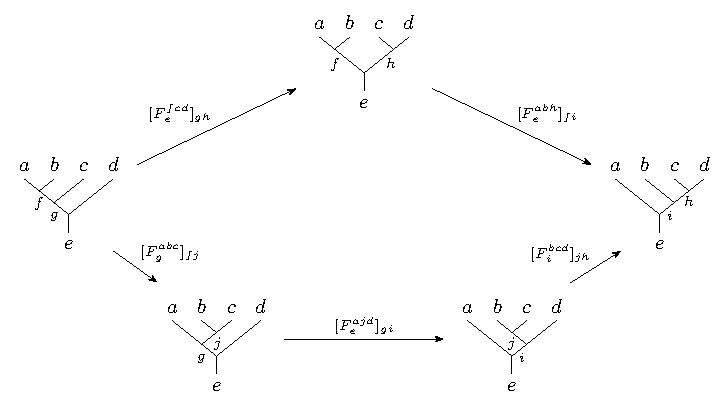
\includegraphics{images/f-symbols-pentagon-equation.pdf}
  \caption[$F$ 符号所满足的五边形方程]{$F$ 符号所满足的五边形方程,对应的融合空间是 $\Hom_{\mathcal{C}}(a\otimes b\otimes c\otimes d,e)$,即 $V^{abcd}_e$。}
  \label{fig:f-symbols-pentagon-equation}
\end{figure}

一个融合范畴可由以下几组数据完全确定:
\begin{itemize}
  \item 简单对象(等价类)的集合 $\{a,b,c,\dots\}$;
  \item 融合系数 $N_{ab}^c$ 或者对应的融合规则;
  \item $F$ 符号 $[F^{abc}_d]_{xy}$。
\end{itemize}
利用这些数据可以对任意弦图进行化简或求值。如果一个弦图没有端点(即“外腿”),那么它的化简结果将是一个复数。根据上文,我们可以进行的操作有:
\begin{itemize}
  \item 任意的连续变形,这是由刚性公理式~\eqref{eq:rigidity-axioms-diagrams} 和自对偶性保证的;
  \item $F$ 移动,即式~\eqref{eq:f-move};
  \item 环路消除,这会得到相应的量子维数:
    \begin{equation}
      \tikzinput{loop-removal-1}
      \! = d_a, \quad
      \tikzinput{loop-removal-2}
      \! = \delta_{ac} \sqrt{\frac{d_b d_{b'}}{d_a}} \enspace
      \tikzinput{loop-removal-3}.
    \end{equation}
\end{itemize}

\subsection{融合范畴的例子}
\label{subsec:fusion-category-examples}

下面我们给出一些融合范畴的例子\cite{rowell2009classification}。这里只列出了非平凡的 $F$ 符号,对于其他合法的融合树,它们之间基变换的 $F$ 符号都等于 1。

\paragraph{Semion}

\begin{itemize}
  \item 简单对象:$\{\1, s\}$;
  \item 量子维数:$d_{\1}=d_s=1$;
  \item 总量子维数:$D=\sqrt2$;
  \item 融合规则:
    \begin{fusionrules}{|c|cc|}
      $\otimes$ & $\1$ & $s$  \\ \hline
      $\1$      & $\1$ & $s$  \\
      $s$       & $s$  & $\1$ \\
    \end{fusionrules}
  \item $F$ 符号:$[F^{sss}_s]_{\1\1}=-1$。
\end{itemize}

\paragraph{Fibonacci}

\begin{itemize}
  \item 简单对象:$\{\1, \tau\}$;
  \item 量子维数:$d_{\1}=1, \, d_\tau=\varphi$;
  \item 总量子维数:$D=\sqrt{\frac{5+\sqrt5}{2}}=2\cos\frac{\pi}{10}$;
  \item 融合规则:
    \begin{fusionrules}{|c|cc|}
      $\otimes$ & $\1$   & $\tau$ \\ \hline
      $\1$      & $\1$   & $\tau$ \\
      $\tau$    & $\tau$ & $\1\oplus\tau$ \\
    \end{fusionrules}
  \item $F$ 符号:
    $
      [F^{\tau\tau\tau}_\tau]_{ij} = \dfrac1\varphi \begin{pmatrix} 1 & \sqrt\varphi \\ \sqrt\varphi & -1 \end{pmatrix}, \,
      i,j \in \{\1, \tau\}
    $。
\end{itemize}

这里的 $\varphi=(1+\sqrt5)/2$ 是黄金比\cite{trebst2008short}。

\paragraph{Ising}

\begin{itemize}
  \item 简单对象:$\{\1, \sigma, \psi\}$;
  \item 量子维数:$d_{\1}=d_\psi=1, \, d_\sigma=\sqrt2$;
  \item 总量子维数:$D=2$;
  \item 融合规则:
    \begin{fusionrules}{|c|ccc|}
      $\otimes$ & $\1$     & $\sigma$       & $\psi$   \\ \hline
      $\1$      & $\1$     & $\sigma$       & $\psi$   \\
      $\sigma$  & $\sigma$ & $\1\oplus\psi$ & $\sigma$ \\
      $\psi$    & $\psi$   & $\sigma$       & $\1$     \\
    \end{fusionrules}
  \item $F$ 符号:
    $
      [F^{\psi\sigma\psi}_\sigma]_{\sigma\sigma} = [F^{\sigma\psi\sigma}_\psi]_{\sigma\sigma} = -1, \,
      [F^{\sigma\sigma\sigma}_\sigma]_{ij} = -\dfrac{1}{\sqrt2} \begin{pmatrix} 1 & 1 \\ 1 & -1 \end{pmatrix}, \,
      i,j \in \{\1, \psi\}
    $。
\end{itemize}

\paragraph{Toric code}

\begin{itemize}
  \item 简单对象:$\{\1, e, m, f\}$;
  \item 量子维数:$d_{\1}=d_e=d_m=d_f=1$;
  \item 总量子维数:$D=2$;
  \item 融合规则:
    \begin{fusionrules}{|c|cccc|}
      $\otimes$ & $\1$ & $e$  & $m$  & $f$  \\ \hline
      $\1$      & $\1$ & $e$  & $m$  & $f$  \\
      $e$       & $e$  & $\1$ & $f$  & $m$  \\
      $m$       & $m$  & $f$  & $\1$ & $e$  \\
      $f$       & $f$  & $m$  & $e$  & $\1$ \\
    \end{fusionrules}
  \item $F$ 符号:都等于 1。
\end{itemize}

\subsection{更复杂的例子:\texorpdfstring{$\mathcal{A}_{k+1}$}{𝒜ₖ₊₁} 范畴}
\label{subsec:A-k+1-category}

$\mathcal{A}_{k+1}$ 范畴\cite{coquereaux2007racah,aasen2020topological,chen2022galois}也称 $\mathfrak{su}(2)_k$ 模型,它最初来自于对 Lie 代数表示的研究。该范畴中共有 $k+1$ 个简单对象,标记为 $0,\frac12,1,\dots,\frac k2$,对应的量子维数为
\begin{equation}
  d_i = \frac{\sin\frac{(2i+1)\pi}{k+2}}{\sin\frac{\pi}{k+2}}, \quad i = 0,1,2,\dots,k.
\end{equation}
计算可得总量子维数
\begin{equation}
  D = \frac12 \left( \cot^2 \frac{\pi}{2k+4} - 1 \right).
\end{equation}
融合规则由下式确定:
\begin{equation}
  N_{ab}^c = \begin{cases}
    1, & a+b\geqslant c, \, b+c\geqslant a, \, c+a\geqslant b, \, a+b+c\leqslant k, \, a+b+c\in\mathbb{Z}; \\
    0, & \text{otherwise}.
  \end{cases}
\end{equation}
例如当 $k=1$ 和 2 时,融合规则分别为
\begin{fusionrules}{|c|cc|}
  $\otimes$ & 0 & ½ \\ \hline
  0         & 0 & ½ \\
  ½         & ½ & 0 \\
\end{fusionrules}
和
\begin{fusionrules}{|c|ccc|}
  $\otimes$ & 0 & ½          & 1 \\ \hline
  0         & 0 & ½          & 1 \\
  ½         & ½ & $0\oplus1$ & ½ \\
  1         & 1 & ½          & 0 \\
\end{fusionrules}。

\begin{equation}
  G^{abc}_{def} = \begin{Bmatrix} a & b & c \\ d & e & f \end{Bmatrix}_q (-1)^p,
\end{equation}
式中
\begin{equation}
  p = \frac{3(a+b+c+d+e+f)^2 - (a+d)^2 - (b+e)^2 - (c+f)^2}{2},
\end{equation}
而 $\{\dots\}_q$ 称为 \emph{$q$-变形 Wigner $6j$ 符号} ($q$-deformed Wigner $6j$ symbol),其定义为
\begin{align}
  \begin{Bmatrix} j_1 & j_2 & j_3 \\ j_4 & j_5 & j_6 \end{Bmatrix}_q
  &= \Delta(j_1,j_2,j_3) \, \Delta(j_1,j_5,j_6) \, \Delta(j_4,j_2,j_6) \, \Delta(j_4,j_5,j_3) \notag \\
  &\times \sum_{z=m}^M \frac{(-1)^z [z+1]!}{[z-a_1]![z-a_2]![z-a_3]! [b_1-z]![b_2-z]![b_3-z]!},
\end{align}
其中
\begin{align}
  q    &= \exp\frac{2\pi\ii}{k+2}, \\
  [n]  &= \frac{q^{m/2} - q^{-m/2}}{q^{1/2} - q^{-1/2}} = \frac{\sin\frac{n\pi}{k+2}}{\sin\frac{\pi}{k+2}}, \\
  [n]! &= \begin{cases}
    \prod_{i=1}^{n} [n], & n \geqslant 1; \\
    1                    & n = 0,
  \end{cases} \\
  \Delta(x,y,z) &= \sqrt{\frac{[x+y-z]! [y+z-x]! [z+x-y]!}{[x+y+z+1]!}},
\end{align}
此外 $a_1=j_1+j_2+j_3$,$a_2=j_1+j_5+j_6$,$a_3=j_2+j_4+j_6$,$a_4=j_3+j_4+j_5$,$b_1=j_1+j_2+j_4+j_5$,$b_2=j_2+j_3+j_5+j_6$,$b_3=j_1+j_3+j_4+j_6$,而对 $z$ 的求和为从 $m=\max\{a_1,a_2,a_3,a_4\}$ 到 $M=\min\{b_1,b_2,b_3\}$ 的整数。

\subsection{模张量范畴与共形场论}

在二维共形场论 (conformal field theory, CFT) 的最小模型 (minimal model) 中,初级场 (primary field) 之间也存在融合规则\cite{ginsparg1988applied,francesco2012conformal}:
\begin{equation}
  \phi_{(r,s)} \times \phi_{(m,n)}
  = \sum_{\substack{k=1+|r-m| \\ k+r+m=1 \bmod 2}}^{k_{\max}} \,
    \sum_{\substack{l=1+|s-n| \\ l+s+n=1 \bmod 2}}^{l_{\max}} \phi_{(k,l)},
\end{equation}
式中
\begin{equation}
  \begin{aligned}
    k_{\max} &= \min(r+m-1, 2p'-1-r-m), \\
    l_{\max} &= \min(s+n-1, 2p-1-s-n),
  \end{aligned}
\end{equation}
而 $p$ 和 $p'$ 是两个互素的整数,它们确定了最小模型 $\mathcal{M}(p,p')$。以二维临界 Ising 模型为例,它是最小模型 $\mathcal{M}(4,3)$,其中的初级场除了恒等算符 $\1$ 之外,还包括自旋 $\sigma$ 和能量密度 $\epsilon$。它们满足的融合规则为:
\begin{equation}
  \sigma\times\sigma = \1+\epsilon, \quad
  \sigma\times\epsilon = \sigma, \quad
  \epsilon\times\epsilon = \1.
\end{equation}
这与上面 Ising 融合范畴中(非平凡)的融合规则是完全一致的。

事实上,我们在 \ref{subsec:fusion-category-examples} 和 \ref{subsec:A-k+1-category} 小节中给出的这几个例子不仅是融合范畴,还是所谓\emph{模张量范畴} (modular tensor category, MTC)\cite{bakalov2001lectures,kitaev2006anyons,bruillard2016rank,beer2018categories,kong2022invitation}。它在融合范畴的基础上加入了\emph{编织} (braiding)、\emph{丝带} (ribbon) 的结构以及\emph{非简并} (non-degeneracy) 的条件,其中定义了\emph{扭转} (twist):
\begin{equation}
  \theta_x = \tikzinput{twist} \, , \quad x \in \mathcal{C},
\end{equation}
\emph{$S$ 矩阵} ($S$ matrix):
\begin{equation}
  S_{ij} = \frac1D \, \tikzinput{s-matrix}, \quad i,j \in I,
\end{equation}
\emph{Gauss 和} (Gauss sums):
\begin{equation}
  p^{\pm} = \sum_{i\in I} \theta_i^{\pm1} d_{i}^2.
\end{equation}
Gauss 和与 $\mathcal{C}$ 的总量子维数相关:
\begin{equation}
  p^+ p^- = D^2,
\end{equation}
而其比值定义为
\begin{equation}
  \zeta = \left( \frac{p^+}{p^-} \right)^{1/6}.
\end{equation}
可以证明模张量范畴中融合系数与 $S$ 矩阵之间存在如下关系\cite{verlinde1988fusion,bakalov2001lectures,huang2005vertex,bruillard2016rank}:
\begin{equation}
  N_{ij}^k = \sum_r \frac{S_{ir} S_{jr} S_{k^\vee r}}{S_{\1 r}},
\end{equation}
这被称为 \emph{Verlinde 公式} (Verlinde formula)。此外,还存在 \emph{Vafa 定理} (Vafa's theorem),即 $\theta_i$ 和 $\zeta$ 都是单位根\cite{bakalov2001lectures}。此时令
\begin{equation}
  \theta_i = \ee^{2\pi\ii\Delta_i}, \quad
  \zeta = \ee^{2\pi\ii c/24},
\end{equation}
% TODO: $\Delta_i$ conformal or scaling dimension?
可知式中 $\Delta_i$ 和 $c$ 都是有理数。它们正是\emph{有理共形场论} (rational CFT, RCFT) 中的\emph{共形维数} (conformal dimension) 和\emph{中心荷} (central charge)。

\section{拓扑序与弦网模型}

\subsection{拓扑序}

在 Landau 相变理论中,不同的相可根据对称性来确定,并可通过\emph{序参量} (order parameter) 来刻画。相变则通过对称性破缺来描述。但在 20 世纪 80 年代以来,随着分数量子 Hall 效应、高温超导等现象的发现,人们意识到 Landau 的对称性破缺理论并不足以描述所有的物态。\emph{拓扑序} (topological order) 的提出即为了描述这些物态的性质,并对其进行分类。

在 2+1D 中,拓扑序可由下面两条性质来确定\cite{zeng2019introduction}:
\begin{itemize}
  \item 基态的拓扑简并;
  \item 非 Abel 的几何相。
\end{itemize}

\subsection{Toric code 模型}

拓扑序的一个基本且重要的例子是 Toric code 模型\cite{kitaev2003fault}。它定义在一个二维正方形网格 (square lattice) 上,每条边上都存在一个自旋 $1/2$ 的自由度 $\sigma_i$。一般我们选取周期性边界条件,即环面拓扑。其 Hamilton 量定义为
\begin{equation}
  H = -\sum_{\bm{v}} A_{\bm{v}} - \sum_{\bm{p}} B_{\bm{p}}, \quad
  A_{\bm{v}} = \prod_{i\in\operatorname{star}(\bm{v})} \sigma_i^x, \quad
  B_{\bm{p}} = \prod_{i\in\operatorname{boundary}(\bm{p})} \sigma_i^z,
  \label{eq:toric-code-hamiltonian}
\end{equation}
其中 $\sum_{\bm{v}}$ 和 $\sum_{\bm{p}}$ 分别表示对所有的顶点 (vertex) 和方块\footnote{在其他网格中也可以是其他形状。} (plaquette) 求和,如图~\ref{fig:toric-code-vertex-plaquette} 所示。

\begin{figure}[htb]
  % TODO: update image
  \centering
  \includegraphics[width=0.5\textwidth]{images/temp/ToricCodeLattice.png}
  \caption[Toric code 中的顶点和方块]{正方形网格上 Toric code 中的顶点 ($\bm{v}$) 和方块 ($\bm{p}$),它们各包含 4 个自旋自由度。}
  \label{fig:toric-code-vertex-plaquette}
\end{figure}

Toric code 中存在 $e$ 和 $m$ 两种激发态,分别由 $\sigma^z$ 和 $\sigma^x$ 组成的弦算符产生。$e$ 和 $m$ 分别绕对方一圈(e.g. $e$ 闭弦 + $m$ 开弦),会给出 -1 的相位。

Toric code 存在 4 种任意子:$\1$、$e$、$m$、$f=e\times m$。它们的 fusion rules 如下……

基态简并度与空间底流形的拓扑有关:$d=2^{2^g}=4^g$,其中 $g$ 为空间的\emph{亏格} (genus)。

\subsection{弦网模型}

\emph{弦网模型} (string-net model)\cite{levin2005string,levin2006detecting} 可以视为 Toric code 模型的一种推广,它是通过 \ref{sec:tensor-category-fusion-category} 节介绍的张量融合范畴来定义的\footnote{准确来说要求模张量范畴。}。弦网模型一般定义在一个三分支 (trivalent) 的网格上,网格的边上带有“弦”的自由度。对于一个具体的弦网模型,我们需要给出下列几组数据:
\begin{itemize}
  \item \emph{弦的类型},按照量子力学的语言也被称为\emph{超选择分区} (superselection sector),它相当于融合范畴中简单对象的集合;
  \item \emph{弦的取向},相当于指定了简单对象的对偶;
  \item \emph{分支规则},相当于融合规则,规定了哪些弦允许汇聚于一点。
\end{itemize}

根据张量融合范畴的精神,弦网模型的基态波函数 $\Phi$ 应该满足下面的约束条件:
\begin{equation}
  % TODO: update image and conventions
  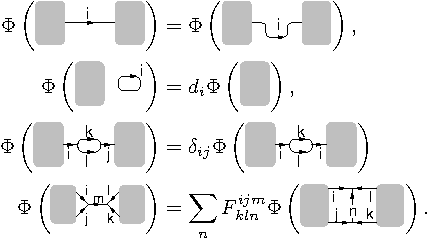
\includegraphics{images/temp/string-net-wave-function.pdf}
\end{equation}
这里的 $F^{ijm}_{kln}$ 是 $F$ 符号的另一种记法,它与 $F[...]$ 的关系将在 [...] 中给出。

在六边形网格 (hexagonal lattice) 上定义的弦网模型,其 Hamilton 量由下式给出:
\begin{equation}
  H = -\sum_{\bm{v}} A_{\bm{v}} - \sum_{\bm{p}} B_{\bm{p}}.
  \label{eq:string-net-hamiltonian}
\end{equation}
与式~\eqref{eq:toric-code-hamiltonian} 类似,这里 $\bm{v}$ 和 $\bm{p}$ 也表示顶点和方块。$A_{\bm{v}}$ 称为\emph{电荷算符} (electric charge operator):
\begin{equation}
  % A_{\bm{v}} \ket{...} = \delta_{ijk} \ket{...}
  \includegraphics{images/temp/string-net-electric-charge.pdf}
\end{equation}
$B_{\bm{p}}$ 称为\emph{磁通量算符} (magnetic flux operator):
\begin{equation}
  B_{\bm{p}} = \sum_{s=0}^N \frac{d_s}{D} B_{\bm{p}}^s,
\end{equation}
其中
\begin{equation}
  \begin{gathered}
    % B_{\bm{p}}^s \ket{...} = \sum ... \ket{...}
    \includegraphics{images/temp/string-net-magnetic-flux.pdf}, \\
    B_{\bm{p},ghijkl}^{s,g'h'i'j'k'l'}(abcdef) =
      F^{al^*g}_{s^*g'l'^*}
      F^{bg^*h}_{s^*h'g'^*}
      F^{ch^*i}_{s^*i'h'^*}
      F^{di^*j}_{s^*j'i'^*}
      F^{ej^*k}_{s^*k'j'^*}
      F^{fk^*l}_{s^*l'k'^*}.
  \end{gathered}
\end{equation}
可以验证 $A_{\bm{v}}$ 与 $B_{\bm{p}}$ 是对易的,因而 Hamilton 量式~\eqref{eq:string-net-hamiltonian} 严格可解。

\chapter{张量网络方法介绍}
\label{chap:tensor-network}

\emph{张量网络} (tensor network)\cite{orus2014practical,bridgeman2017hand,biamonte2017tensor,orus2019tensor,ran2020tensor,evenbly2022practical}方法为凝聚态物理、量子计算\cite{markov2008simulating,huggins2019towards,yuan2021quantum}、机器学习\cite{stoudenmire2016supervised,you2018machine,liu2023tensor}\allowbreak 与可微编程\cite{liao2019differentiable,geng2022differentiable}等领域提供了一套统一的描述框架。顾名思义,张量网络就是根据一定规则连接起来张量单元,而这些局域的张量单元往往能够编码全局波函数的关键性质。相比传统的数值算法,张量网络将刻画量子态的关联与纠缠性质放在了第一优先级,因而在处理复杂的量子多体问题也具有很强的表达能力。

\section{基本概念}

张量网络中的\emph{张量} (tensor) 可以简单理解为多维数组,即标量(0 维张量)、向量(1 维张量)、矩阵(2 维张量)的推广。如图~\ref{fig:tensors} 所示,张量网络常利用图形方式来描述,其中圆圈(也可用其他图形)表示张量,延伸出来的腿表示张量的指标。

\begin{figure}[htb]
  \centering
  \tikzinput{tensor-network/basic}
  \caption[张量单元]{三种张量单元,分别对应于向量、矩阵和三阶张量。}
  \label{fig:tensors}
\end{figure}

\subsection{基本张量运算}

常用的张量运算包括张量积、缩并、变形等。

\emph{张量积} (tensor product) 相当于若干个张量并排放置,并保持指标不变:
\begin{equation}
  A_{i_1,\dots,i_r} B_{j_1,\dots,j_s} \eqcolon (A \otimes B)_{i_1,\dots,i_r,j_1,\dots,j_s}.
\end{equation}
图形描述为
\begin{equation}
  \tikzinput{tensor-network/tensor-product}
\end{equation}

张量的\emph{缩并} (contraction) 是向量内积、矩阵乘法的推广,即对两个张量的某些指标进行求和,得到一个新的张量:
\begin{equation}
  A_{abk} B_{kc} \coloneq \sum_k A_{abk} B_{kc} = C_{abc}.
\end{equation}
这里根据 Einstein 求和约定省略了求和号。张量缩并的图形描述为
\begin{equation}
  \tikzinput{tensor-network/contraction}
\end{equation}
即把需要缩并的腿(指标)连接起来。

同一个张量的指标也可以缩并。部分缩并可以得到\emph{偏迹} (partial trace),全部缩并则得到\emph{迹} (trace):
\begin{align}
     (\tr_{x,y} A)_{i_1,\dots,i_{x-1},i_{x+1},\dots,i_{y-1},u_{y+1},\dots,i_r}
  &= A_{i_1,\dots,i_{x-1},k,i_{x+1},\dots,i_{y-1},k,i_{y+1},\dots,i_r}, \\
     \tr B
  &= B_{ii}
\end{align}
其图形描述与缩并类似:
\begin{equation}
  \tikzinput{tensor-network/trace-1}
\end{equation}
利用图形语言很容易验证 $\tr(AB)=\tr(BA)$:
\begin{equation}
  \tikzinput{tensor-network/trace-2}
\end{equation}

张量的\emph{变形} (reshape) 相当于指标的重新组合,例如
\begin{equation}
  \tikzinput{tensor-network/reshape}
\end{equation}
在数值计算中,把一般形状的张量变形为矩阵,往往可以利用为矩阵优化的算法来加速计算。

\subsection{张量分解}

张量的\emph{分解} (decomposition) 可以理解为缩并的逆运算,最常用的是\emph{奇异值分解} (singular value decomposition, SVD),即
\begin{equation}
  M_{ij} = \sum_{k=1}^{\min(m,n)} U_{ik} \Lambda_{kk} V_{kj} = \sum_k U_{ik} \Lambda_{kk} \bigl( V^\dagger \bigr)_{jk},
\end{equation}
其中 $M$ 为 $m\times n$ 矩阵,$\Lambda$ 为对角矩阵(如果行数、列数不等,则相应补零),$U$ 和 $V$ 为幺正矩阵,$V^\dagger$ 表示共轭转置。利用张量的变形,可以很容易地将 SVD 推广为一般形状的张量,用图形描述为
\begin{equation}
  \tikzinput{tensor-network/svd}
\end{equation}

奇异值分解可以用来获得张量的近似表示。将奇异值($\Lambda$ 矩阵的对角元)按大小排列后,只保留前 $r$ 个值,就得到了秩为 $r$ 的近似张量:
\begin{equation}
  M_{ij} \approx \sum_{k=1}^r U_{ik} \Lambda_{kk} V_{kj}, \quad r < \min(m,n).
\end{equation}
并且可以证明,这种近似表示是所有秩为 $r$ 的张量中最优的。

对于一个一般的张量,原则上我们总可以把它改写为若干个小张量的缩并形式,并保证自由度数目不变。这种改写并不能降低计算复杂度,但我们可以利用奇异值分解把这些小张量替换为对应的近似表示,这样就可以大幅减少总自由度的数目。

在量子力学的语境中,奇异值分解也可表述为 \emph{Schmidt 分解} (Schmidt decomposition):对于 Hilbert 空间 $\mathcal{H}^{\text{L}}\otimes\mathcal{H}^{\text{R}}$,其中的任意量子态 $\ket{\Psi}$ 均可被分解为
\begin{equation}
  \ket{\Psi} = \sum_\alpha \lambda_\alpha \ket{\Phi^{\text{L}}_\alpha} \otimes \ket{\Phi^{\text{R}}_\alpha},
  \label{eq:schmidt-decomposition}
\end{equation}
其中 $\lambda_\alpha$ 称为 \emph{Schmidt 系数} (Schmidt coefficients),而 $\ket{\Phi^{\text{L}}_\alpha}$、$\ket{\Phi^{\text{R}}_\alpha}$ 分别是 $\mathcal{H}^{\text{L}}$、$\mathcal{H}^{\text{R}}$ 中的单位正交基,称为 \emph{Schmidt 向量} (Schmidt vectors)。可以发现 Schmidt 系数和奇异值是等价的,而 Schmidt 向量和幺正矩阵 $U$、$V$ 也是等价的。

\section{矩阵乘积态算法}

接下来介绍几种具体的张量网络及其算法。本文中,我们把这些算法分为两类:一类算法以矩阵乘积态为代表,主要用来处理一维量子多体系统;另一类算法则以张量重整化群为代表,顾名思义,主要用在二维网络的重整化(粗粒近似)操作中。

\subsection{波函数的构造}
\label{subsec:mps-construction}

如图~\ref{fig:mps} 所示,\emph{矩阵乘积态} (matrix product state, MPS)\cite{perez2007matrix,verstraete2008matrix,orus2014practical,cirac2021matrix}由一系列张量单元首尾相连而成,每个张量单元包含三个指标,没有缩并的称为\emph{物理指标} (physical index),另外两个则称为\emph{虚拟指标} (virtual index) 或\emph{辅助指标} (auxiliary index)。根据具体问题的需要,MPS 可取开放或周期性边界条件。当所研究的系统具有平移对称性时,可以将所有张量单元取为相同值,此时有
\begin{equation}
  % TODO: 周期性边界条件
  \Psi_{i_1 i_2 \cdots i_n} = A^{j_1 j_2}_{i_1} A^{j_2 j_3}_{i_2} \cdots A^{j_n j_1}_{i_n}.
\end{equation}
这样的张量网络称为\emph{无限 MPS} (infinite MPS, iMPS)。
% 我们之后的讨论主要针对 iMPS。

\begin{figure}[htb]
  \centering
  \subcaptionbox{开放边界条件}{\tikzinput{tensor-network/mps-1}} \qquad
  \subcaptionbox{周期性边界条件}{\tikzinput{tensor-network/mps-2}}
  \caption[矩阵乘积态]{矩阵乘积态。}
  \label{fig:mps}
\end{figure}

考虑一个量子态 $\ket{\Psi}$,我们对它作用一次 SVD,便可以获得由两个张量组成的 MPS,此时连接维数 $\chi$ 等于奇异值的数量。这一过程可以不断重复,以构造出任意长度的 MPS。在做 SVD 时,如果不对奇异值进行截断,可以发现 $\chi$ 会随着分解的次数(也即张量单元的数量)$N$ 指数级增长。然而对于一维\emph{有能隙} (gapped) Hamilton 量的基态以及低能激发态,$\chi$ 可以取为常数;对于\emph{无能隙} (gapless) 的临界系统,则会以多项式形式发散。

对于长度为 $L$ 的 MPS,其纠缠熵为
\begin{equation}
  S_L = -\tr(\rho_L\log\rho_L) \sim \mathcal{O}(\log\chi),
\end{equation}
其中 $\rho_L$ 是相应区块上的约化密度矩阵。这和一维有能隙 Hamilton 量基态的性质[称为\emph{面积定律} (area law)]是一致的,因此 MPS 可以较好地模拟这类系统。实际上,在全部 Hilbert 空间中,遵循面积定律的量子态仅占很少的一部分,而张量网络的结构恰好可以排除掉那些“无关”的量子态,从而大大减少了计算量。

由上述方法构造出的 MPS 并不是唯一的,而是存在所谓\emph{规范自由度} (gauge freedom)\cite{bridgeman2017hand}。如图~\ref{fig:mps-gauge-freedom} 所示,两个张量单元之间总可以插入单位矩阵 $I=XX^{-1}$,并把 $X$ 和 $X^{-1}$ 分配到两边。

\begin{figure}[htb]
  \centering
  \tikzinput{tensor-network/gauge-freedom}
  \caption[MPS 中的规范自由度]{MPS 中的规范自由度。其中张量单元 $\tilde{A}=XAX^{-1}$。}
  \label{fig:mps-gauge-freedom}
\end{figure}

% TODO: 密度矩阵
为了方便计算,我们一般会把 MPS 取为\emph{正则形式} (canonical form)\cite{orus2008infinite,schollwock2011density,orus2014practical},它要求辅助指标由 Schmidt 分解式~\eqref{eq:schmidt-decomposition} 决定。张量单元 $A$ 会被拆分成 $\Gamma$ 和 $\lambda$ 两部分,分别对应 Schmidt 向量与系数。定义左右矩阵
\begin{equation}
  \begin{aligned}
       R_{(\alpha\alpha'), \, (\beta\beta')}
    &= \sum_{i=1}^d \left( \Gamma^i_{\alpha\beta} \lambda_\beta \right) \left( \Gamma^i_{\alpha'\beta'} \lambda_{\beta'} \right)^*, \\
       L_{(\alpha\alpha'), \, (\beta\beta')}
    &= \sum_{i=1}^d \left( \lambda_\alpha \Gamma^i_{\alpha\beta} \right) \left( \lambda_{\alpha'} \Gamma^i_{\alpha'\beta'} \right)^*,
  \end{aligned}
\end{equation}
此时正则形式要求 $R$、$L$ 的特征向量均为单位矩阵(在张量变形的意义下),且对应的主特征值\footnote{即绝对值最大的特征值。它对应的特征向量也称主特征向量。} $\eta$ 相同。如图~\ref{fig:mps-canonical-form} 所示,将一般的 $\Gamma$ 和 $\lambda$(例如随机初始化的)进行正则化的方法为:

\begin{enumerate}
  \item 计算 $R$、$L$ 的主特征向量,并变形为矩阵 $V_R$、$V_L$\footnote{在实际计算中,$V_R$、$V_L$ 可能会带有冗余的相位,这会影响接下来的矩阵分解操作。此相位可通过规定 $V_R$、$V_L$ 的迹为实数来消除。},对应的特征值均为 $\eta$。将 $V_R$、$V_L$ 进一步分解为 $X$、$Y$,使其满足
    \begin{equation}
      V_R = X X^\dagger, \quad V_L = Y^\dagger Y.
    \end{equation}
    这里可以用特征值分解,也可以用 Cholesky 分解。

  \item 利用规范自由度在 $\lambda$ 两侧分别插入 $I=(Y^\trans)^{-1}Y^\trans$ 和 $I=XX^{-1}$,并对得到的 $Y^\trans\lambda X$ 进行奇异值分解:
    \begin{equation}
      Y^\trans \lambda X = U \lambda V^\dagger.
    \end{equation}

  \item 将新得到的张量重排为 $\Gamma'$
    \begin{equation}
      \Gamma' = V^\dagger X^{-1} \Gamma \left( Y^\trans \right)^{-1} U.
    \end{equation}
\end{enumerate}

可以证明通过以上步骤得到的 $\Gamma'$ 和 $\lambda'$ 的确是 iMPS 的正则形式。

\begin{figure}[htb]
  \centering
  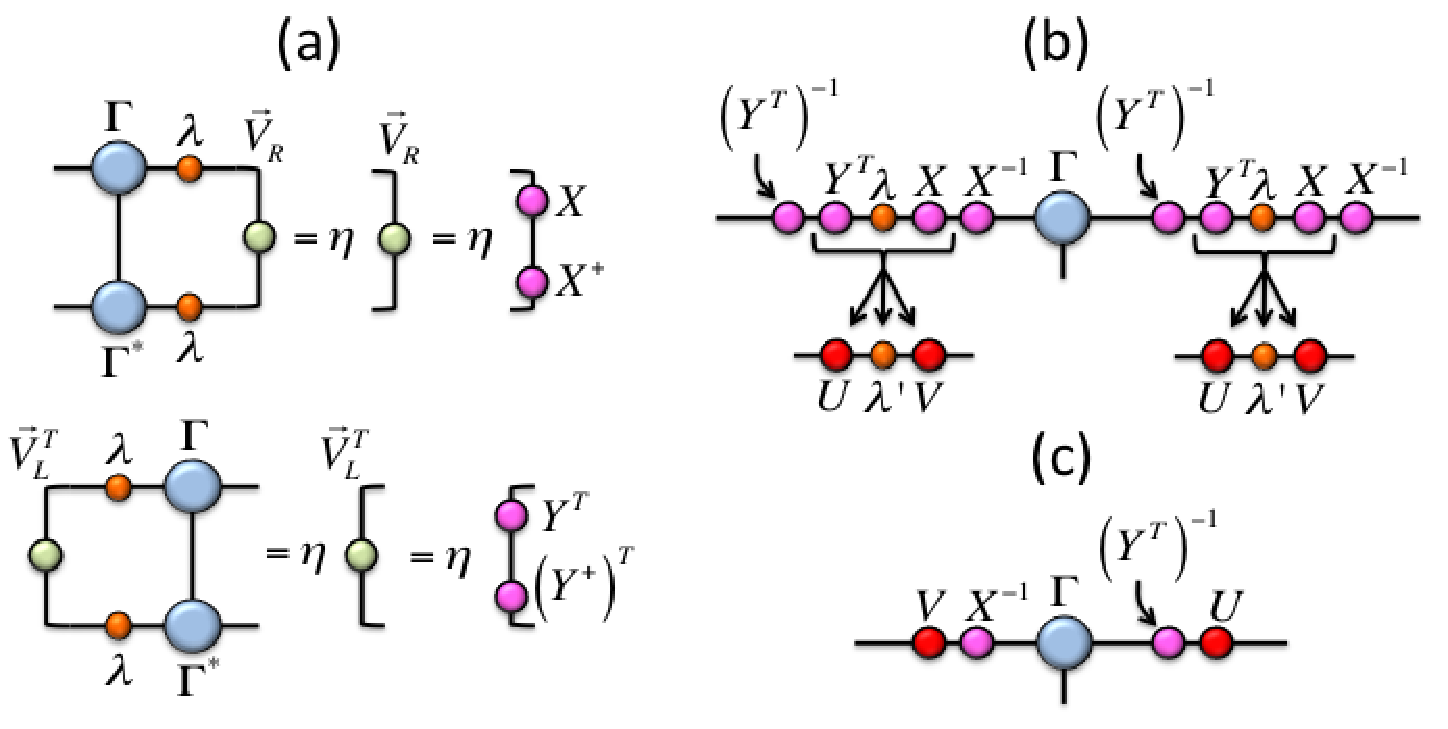
\includegraphics[width=0.85\textwidth]{images/tensor-network/mps-canonical-form.pdf}
  \caption[MPS 的正则形式]{MPS 的正则形式。(a) 计算主特征向量 $V_R$、$V_L$;(b) 利用规范自由度插入 $I=(Y^\trans)^{-1}Y^\trans$ 和 $I=XX^{-1}$,并进行 SVD;(c) 重排张量,得到 $\Gamma'$。图片来源:\parencite{orus2014practical}。}
  \label{fig:mps-canonical-form}
\end{figure}

\subsection{基态的确定}

Hamilton 量的基态 $\Psi_0$ 可以通过变分法求得:
\begin{equation}
  \ket{\Psi_0} = \argmin_{\ket{\Psi}} \frac{\langle\Psi|H|\Psi\rangle}{\langle\Psi|\Psi\rangle}.
\end{equation}
即使 $\ket{\Psi}$ 已经表示成了 MPS 的形式,一般来说也无法直接对 $\ket{\Psi}$ 进行整体优化。但是,如果 Hamilton 量能够写成 MPO 的形式,那么可以通过迭代算法来高效地计算 $H\ket{\Psi}$,进而通过局域优化来获得全局最优解。这实际上就是著名的\emph{密度矩阵重整化群} (density matrix renormalization group, DMRG) 算法\cite{white1992density,white1993density,schollwock2005density,mcculloch2007density,mcculloch2008infinite,schollwock2011density}。

DMRG 的总体思路是,对正则化的 MPS 中每个张量单元 $A^{(i)}$ 依次进行优化,而这里的优化则相当于计算有效 Hamilton 量(原始 Hamilton 量 + MPS 的剩余部分)的本征态。$i$ 由 1 遍历到 $N$ 再遍历回 1 称为一次\emph{扫描} (sweep)。扫描可重复多次,直至 MPS 收敛。

根据 Lagrange 乘子法的精神,定义能量泛函为\footnote{式~\eqref{eq:dmrg-energy-functional}--\eqref{eq:dmrg-normalized-energy-equation} 中图片来源:\parencite{schollwock2011density}。}:
\begin{align}
     E[A, \tilde{A}, \lambda]
  &= \langle \Psi(A)|H|\Psi(A) \rangle - \lambda \langle \Psi(A)|\Psi(A) \rangle \notag \\
  &= \vcenter{\hbox{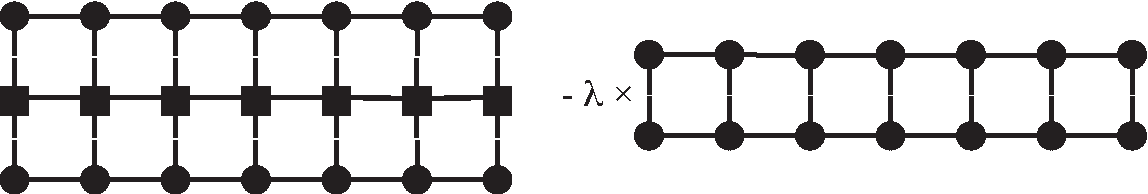
\includegraphics[height=1.7cm]{images/tensor-network/dmrg-energy-functional.pdf}}}.
  \label{eq:dmrg-energy-functional}
\end{align}
其中 $\lambda$ 是 Lagrange 乘子。能量取极小值的(必要)条件为
\begin{equation}
    \pdv{E[A,\tilde{A},\lambda]}{\tilde{A}^{s_i}_{\alpha_i\alpha_{i+1}}}
  = \pdv{}{\tilde{A}^{s_i}_{\alpha_i\alpha_{i+1}}} \langle \Psi(A)|H|\Psi(A) \rangle
  - \lambda \pdv{}{\tilde{A}^{s_i}_{\alpha_i\alpha_{i+1}}} \langle \Psi(A)|\Psi(A) \rangle = 0.
\end{equation}
在张量网络中,由于 $\langle\Psi(A)|H|\Psi(A)\rangle$ 和 $\langle\Psi(A)|\Psi(A)\rangle$ 都可以写成关于 $\tilde{A}^{s_i}_{\alpha_i\alpha_{i+1}}$ 的一次多项式(即其他张量与它的缩并),因此偏导数相当于在整个张量网络中“挖去” $\tilde{A}$ 的结果:
\begin{equation}
  \vcenter{\hbox{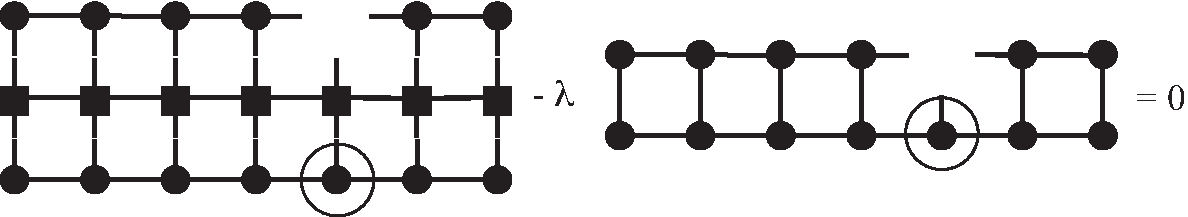
\includegraphics[height=1.9cm]{images/tensor-network/dmrg-energy-equation.pdf}}}.
\end{equation}
由于 MPS 已被正则化($R$、$L$ 的特征向量均为单位向量),上式中的第二项可以被大大简化:
\begin{equation}
  \vcenter{\hbox{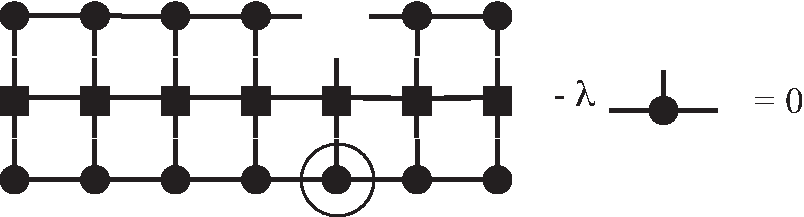
\includegraphics[height=1.9cm]{images/tensor-network/dmrg-normalized-energy-equation.pdf}}}.
  \label{eq:dmrg-normalized-energy-equation}
\end{equation}
此时,我们可以看到上式是一个关于 $A^{s'_i}_{\alpha'_i\alpha'_{i+1}}$(圆圈部分)的特征值方程:
\begin{equation}
  H_{\text{eff}} A = \lambda A,
\end{equation}
而它可以通过标准的特征值求解算法(如 Lanczos 算法)来处理。由此,我们就对 $i$ 位置处的张量单元进行了优化。

为了能够通过连接维数来控制模拟精度和计算效率,如图~\ref{fig:dmrg-two-site} 所示,我们还可以在 DMRG 中同时对两个位置的张量单元进行优化,并且利用 SVD 来得到新的 MPS。

\begin{figure}[htb]
  \centering
  \begin{tabular}{cc}
    \parbox{2em}{\subcaption{}} &
      $\vcenter{\hbox{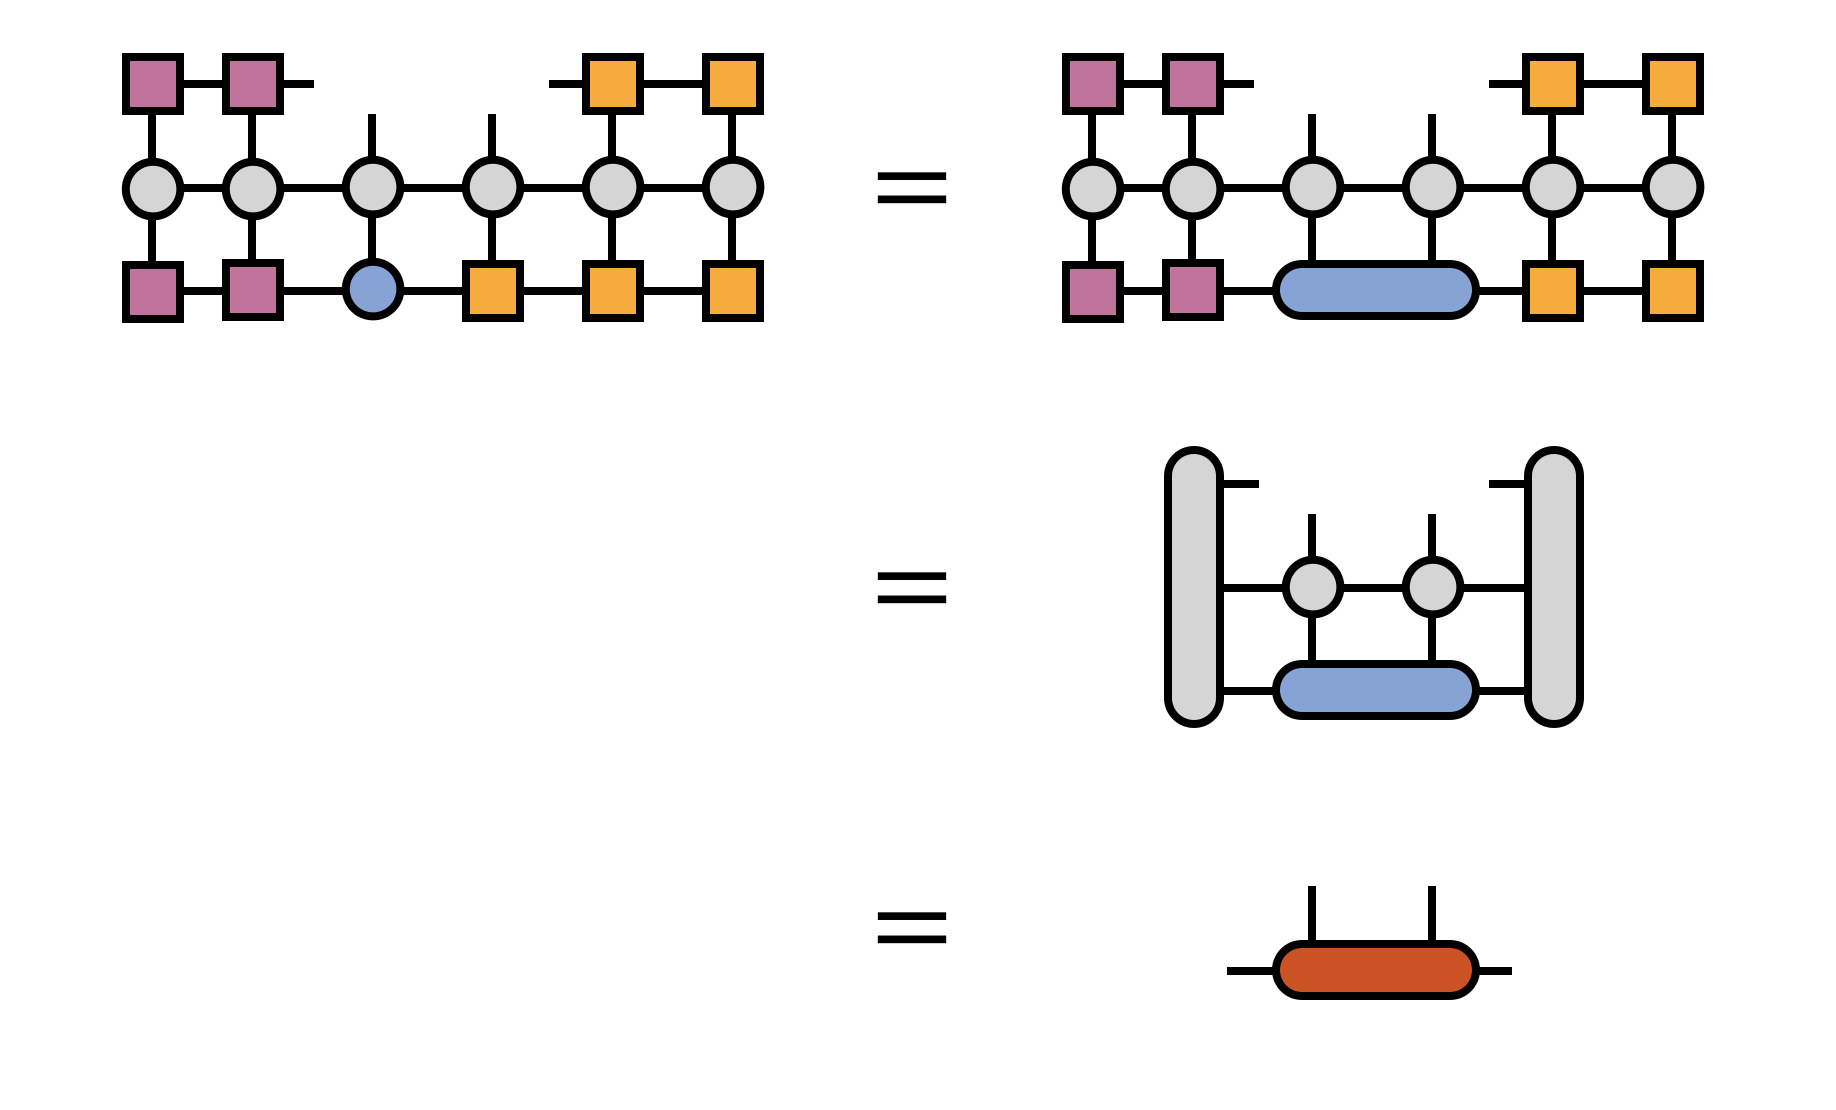
\includegraphics[width=0.7\textwidth]{images/temp/dmrg-two-site.png}}}$ \\
    \parbox{2em}{\subcaption{}} &
      $\vcenter{\hbox{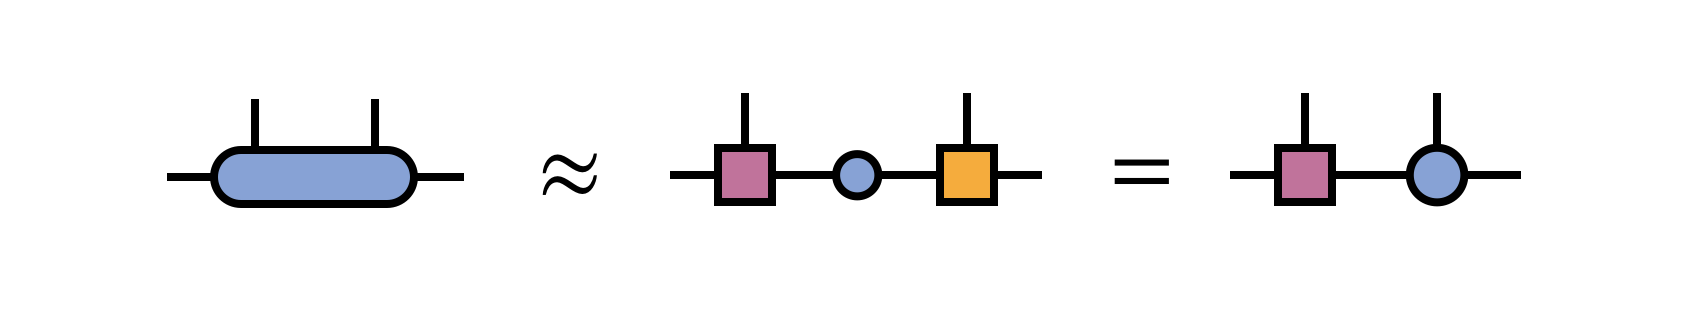
\includegraphics[width=0.7\textwidth]{images/temp/dmrg-two-site-svd.png}}}$
  \end{tabular}
  \caption[两位置上 DMRG 算法]{两位置上 DMRG 算法。(a) 两个 MPS 张量单元首先缩并,再和 $H$ 缩并,得到 $H_{\text{eff}}$。(b) 利用 SVD 来得到新的 MPS。图片来源:\url{https://tensornetwork.org/mps/algorithms/dmrg/}。}
  \label{fig:dmrg-two-site}
\end{figure}

\subsection{时间演化}
\label{subsec:mps-time-evolution}

下面我们介绍\emph{无限时间演化块消减} (infinite time-evolving block decimation, iTEBD)\cite{vidal2007classical,orus2008infinite}算法,它主要用来处理波函数的时间演化
\begin{equation}
  \ket{\Psi_t} = \ee^{-\ii Ht} \ket{\Psi_0}
\end{equation}
或虚时演化
\begin{equation}
  \ket{\Psi_\tau} = \ee^{-H\tau} \ket{\Psi_0},
\end{equation}
其核心在于通过 Suzuki--Trotter 分解\cite{sornborger1999higher}
\begin{equation}
  \ee^{-\tau(A+B)} = \ee^{-\tau A} \ee^{-\tau B} + \mathcal{O}(\tau^2)
\end{equation}
将演化算符表示成 MPO 的形式,这样就可以很方便地与 MPS 形式的波函数进行缩并。

对于时间演化或虚时演化算符而言,由于经过 Suzuki--Trotter 分解后它们都很接近幺正算符,不会破坏 iMPS 的正则形式。而一般的算符并不具备这一性质,所以需要额外进行正则化操作。如图~\ref{fig:itebd-evolution} 所示,一般的 iTEBD 算法如下:

\begin{enumerate}
  \item 取随机的 iMPS $\{\Gamma,\lambda\}$,并按照 \ref{subsec:mps-construction} 小节中介绍的方法将其正则化。

  \item 把 $\{\Gamma,\lambda\}$ 与 MPO 的张量单元进行缩并:
    \begin{equation}
      \tilde{\Gamma}_{j\tilde{\alpha}\tilde{\beta}} = \sum_{i=1}^d \Gamma_{i\alpha\beta} O_{ij\mu\nu}, \quad
      \tilde{\lambda}_{\tilde{\beta}} = \lambda_\beta.
    \end{equation}
    这里指标 $\tilde{\alpha}=(\alpha,\mu)$、$\tilde{\beta}=(\beta,\nu)$,因此得到的 iMPS 对应连接维数 $\tilde{\chi}=\kappa\chi$。

  \item 对 $\{\tilde{\Gamma},\tilde{\lambda}\}$ 进行正则化,得到 $\{\tilde{\Gamma}',\tilde{\lambda}'\}$。

  \item 利用奇异值分解对 $\{\tilde{\Gamma}',\tilde{\lambda}'\}$ 进行截断,即只保留前 $\chi$ 个奇异值,使得连接维数保持在 $\chi$。

  \item 重复步骤 2--4,直到 iMPS 收敛。
\end{enumerate}

\begin{figure}[htb]
  \centering
  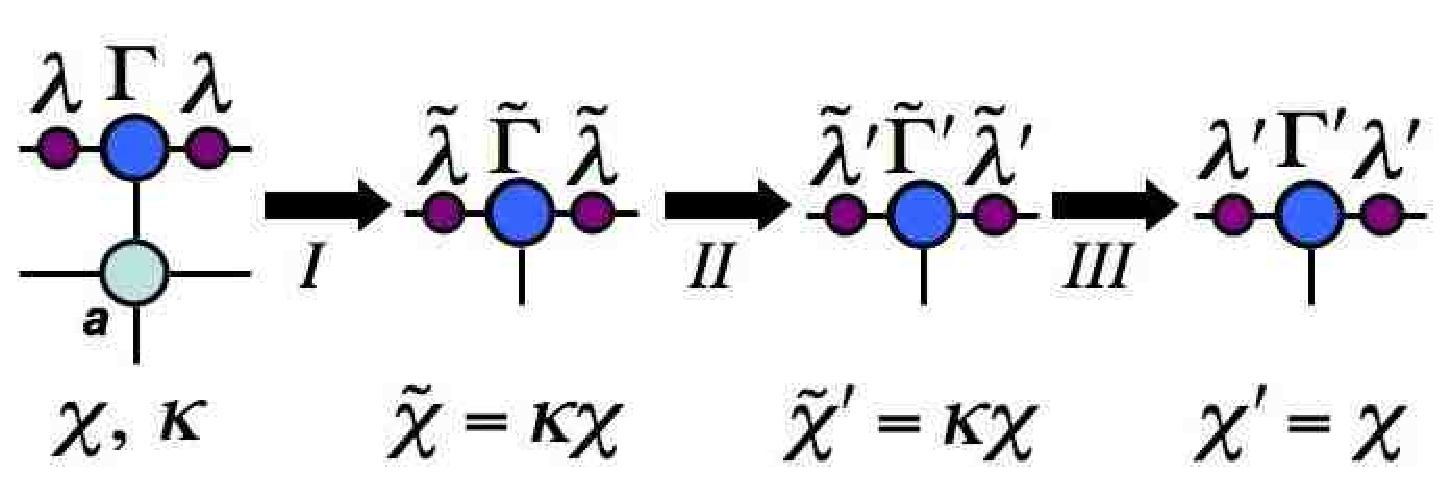
\includegraphics[width=0.6\textwidth]{images/tensor-network/itebd-evolution.pdf}
  \caption[iTEBD 算法]{iTEBD 算法。(I) 把 iMPS $\{\Gamma,\lambda\}$ 与 MPO 的张量单元进行缩并;(II) 对 $\{\tilde{\Gamma},\tilde{\lambda}\}$ 进行正则化;(III) 利用 SVD 把连接维数保持在 $\chi$。图片来源:\parencite{orus2008infinite}。}
  \label{fig:itebd-evolution}
\end{figure}

\subsection{配分函数的计算}
\label{subsec:partition-function}

一个不同于时间(虚时)演化的例子,是把二维经典格点模型的配分函数视为 iMPS 在转移矩阵作用下的演化:
\begin{equation}
  Z(\beta) = \lim_{p,q\to\infty} \omega^{pq},
\end{equation}
其中 $\omega$ 是 $W$ 矩阵的主特征值\cite{orus2008infinite}:
\begin{equation}
  \vcenter{\hbox{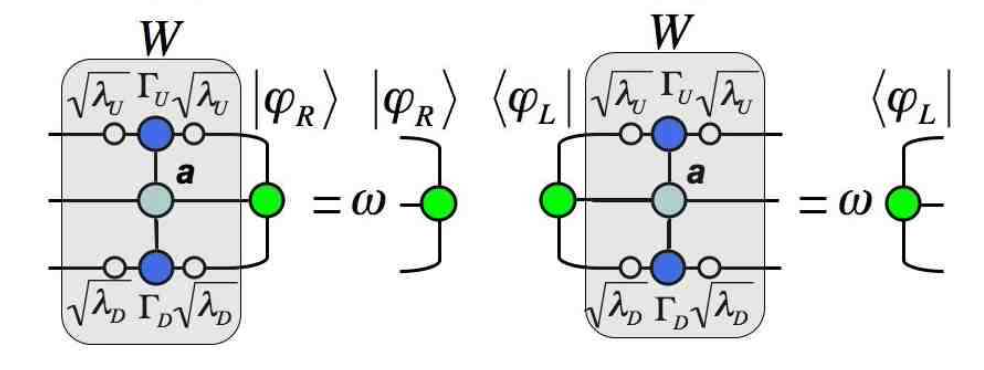
\includegraphics[width=0.7\textwidth]{images/temp/itebd-w-matrices.png}}}
\end{equation}
此时我们还可以计算单点函数和两点(关联)函数的期望值:
\begin{equation}
  \begin{aligned}
    \ev[\big]{f(\sigma^{\bm{r}})}
      &= \frac{1}{Z(\beta)} \sum_{\{\sigma\}} f(\sigma^{\bm{r}}) \, \ee^{-\beta H(\{\sigma\})}, \\
    \ev[\big]{f(\sigma^{\bm{r}}) g(\sigma^{\bm{r}'})}
      &= \frac{1}{Z(\beta)} \sum_{\{\sigma\}} f(\sigma^{\bm{r}}) g(\sigma^{\bm{r}'}) \, \ee^{-\beta H(\{\sigma\})}.
  \end{aligned}
\end{equation}
主要思路是将原配分函数中的张量单元 $A$ 替换为包含 $f(s)$ 或 $g(s)$ 的 $B$ 或 $B'$,并用同样的方法进行缩并。如图~\ref{fig:expectation-value} 所示,由于 iMPS 已被正则化,我们只需处理一个较小的张量网络。

\begin{figure}[htb]
  \centering
  \subcaptionbox{}{%
    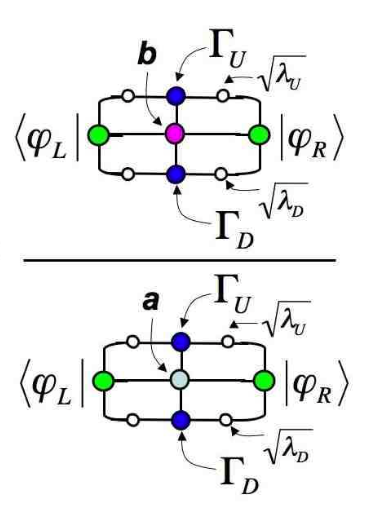
\includegraphics[height=6.5cm]{images/temp/itebd-one-point-function.png}} \quad
  \subcaptionbox{}{%
    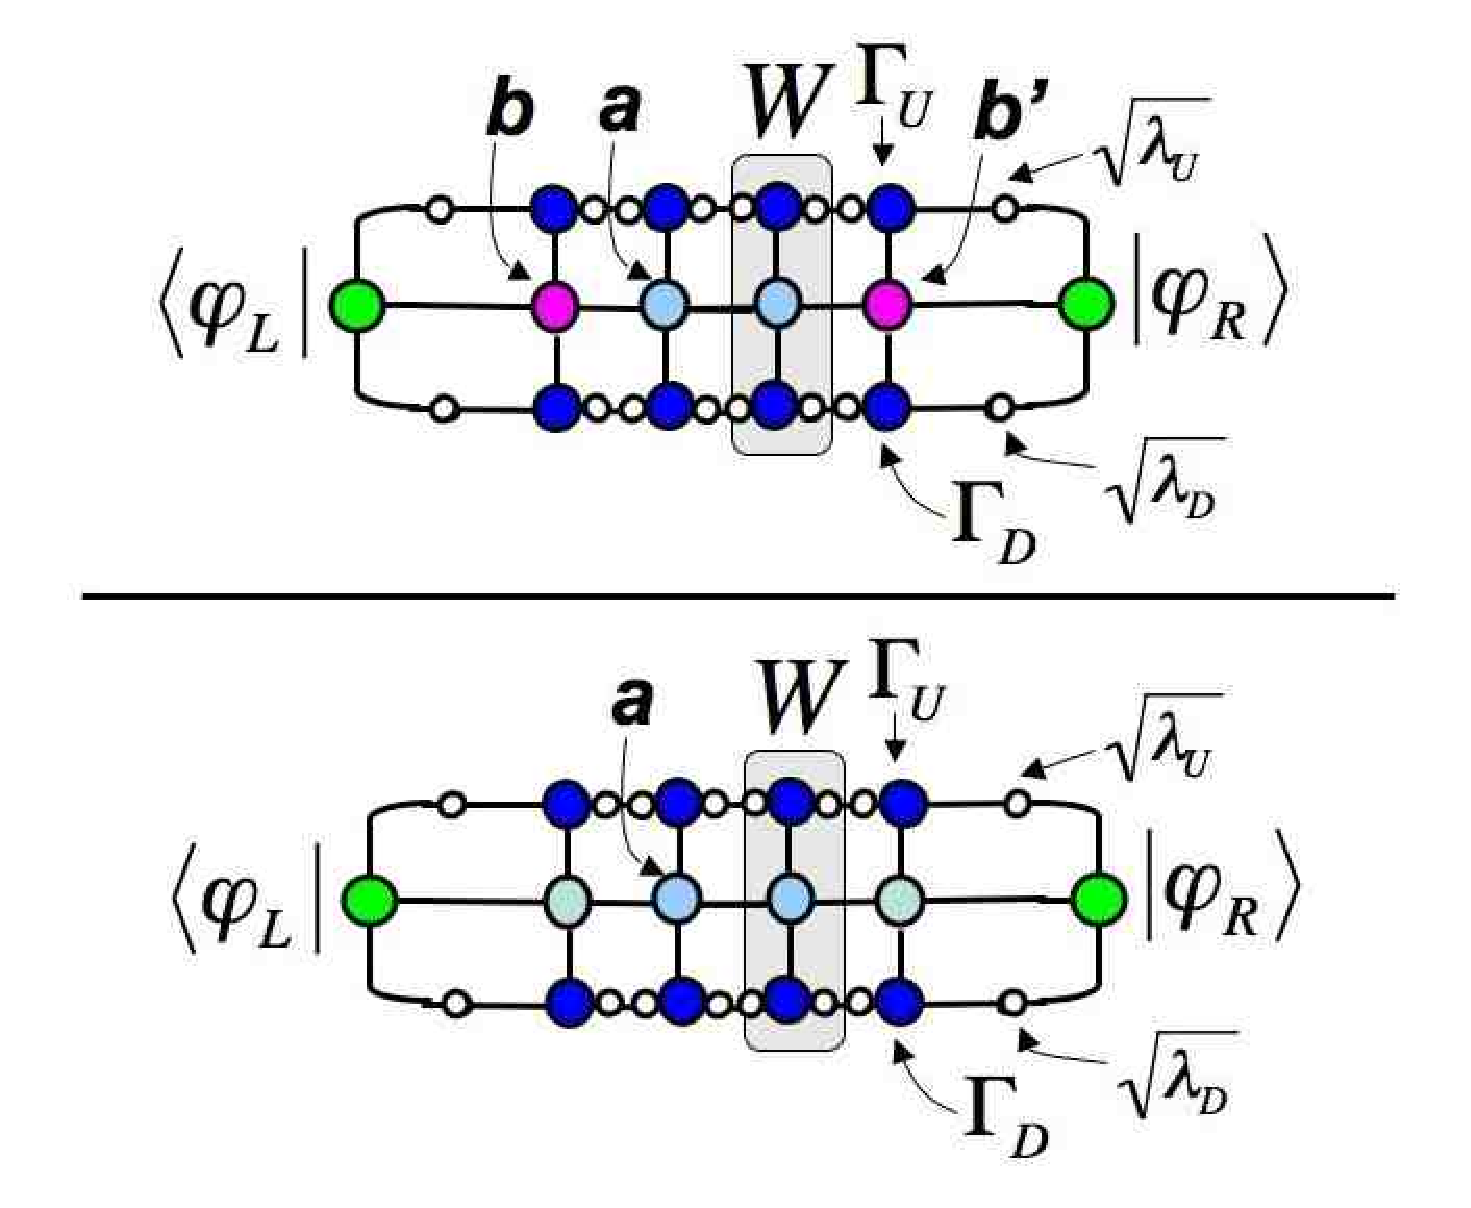
\includegraphics[height=6.5cm]{images/tensor-network/itebd-two-point-function.pdf}}
  \caption[单点函数和两点关联函数的计算]{(a) 单点函数和 (b) 两点(关联)函数的计算。图片来源:\parencite{orus2008infinite}。}
  \label{fig:expectation-value}
\end{figure}

\subsection{推广}
\label{subsec:mps-generalization}

如图~\ref{fig:peps} 所示,MPS 向高维的自然推广就得到了\emph{投影纠缠对态} (projected entangled pair state, PEPS)\cite{verstraete2004renormalization,orus2014practical,cirac2021matrix} 张量网络。对于长宽均为 $L$、连接维数为 $\chi$ 的 PEPS,其纠缠熵满足
\begin{equation}
  S_L \sim \mathcal{O}(L\log\chi),
\end{equation}
这与二维系统的面积定律也是相一致的。此外,PEPS 可以准确描述幂律形式的关联函数,因此可以用来处理一维的量子临界系统(可通过经典—量子模型的映射来实现)。但与一维的 MPS 不同,在 PEPS 中无法为所有指标同时指定一组正交基,因此并不能精确定义正则形式。

\begin{figure}[htb]
  \centering
  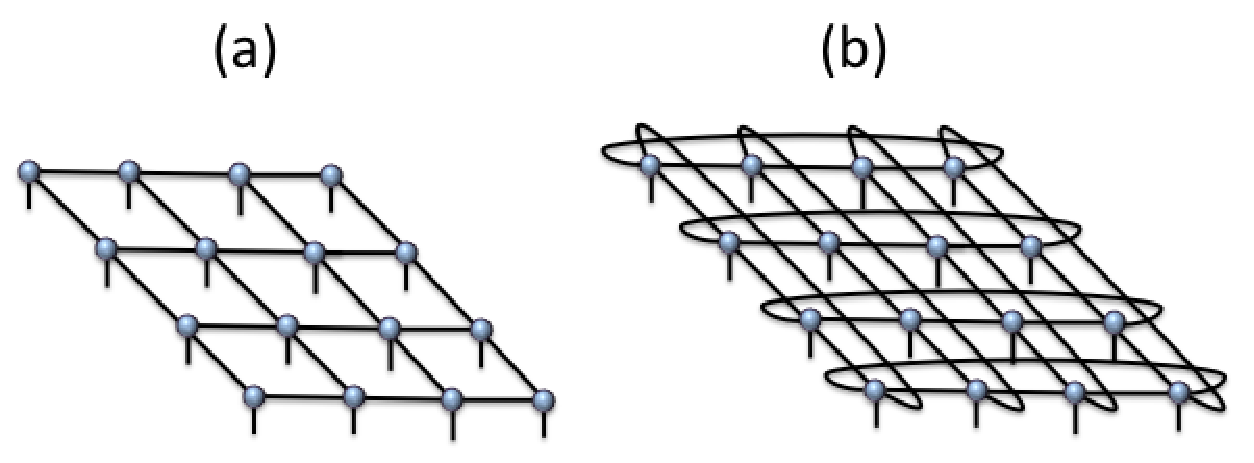
\includegraphics[width=0.8\textwidth]{images/tensor-network/peps.pdf}
  \caption[投影纠缠对态]{投影纠缠对态。图 (a)、(b) 分别对应开放和周期性边界条件。图片来源:\parencite{orus2014practical}。}
  \label{fig:peps}
\end{figure}

另一种用来近似表示一维系统的张量网络是\emph{多尺度纠缠重整化方法} (multiscale entanglement renormalization ansatz, MERA)\cite{vidal2007entanglement,evenbly2009algorithms,konig2009exact,evenbly2014algorithms,evenbly2015tensor2}。如图~\ref{fig:mera} 所示,MERA 使用了一组幺正变换
\begin{equation}
  u \colon \mathbb{V} \otimes \mathbb{V} \to \mathbb{V} \otimes \mathbb{V}, \quad
  u u^\dagger = I^{\otimes2}
\end{equation}
和投影算符
\begin{equation}
  v \colon \mathbb{V} \to \mathbb{V} \otimes \mathbb{V}, \quad
  v^\dagger v = I
\end{equation}
来构建粗粒近似的波函数,其中 $\mathbb{V}=\mathbb{C}^\chi$ 是 $\chi$ 维复向量空间。这里的 $u$ 和 $v$ 分别称为\emph{解纠缠子} (disentangler) 和\emph{等距子} (isometry)。解纠缠子可以消除短程纠缠的影响,因而其纠缠熵满足
\begin{equation}
  S_L \sim \mathcal{O}(\log L).
\end{equation}
这就使得 MERA 张量网络可以较好地近似一维无能隙的临界系统。

\begin{figure}[htb]
  \centering
  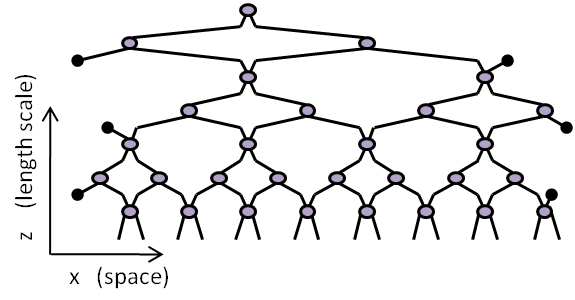
\includegraphics[width=0.6\textwidth]{images/tensor-network/mera.pdf}
  \caption[多尺度纠缠重整化方法]{多尺度纠缠重整化方法。其中两条腿进、两条腿出的张量单元是解纠缠子 $u$,而两条腿进、一条腿出的张量单元则是等距子 $v$。图片来源:\parencite{evenbly2011tensor}。}
  \label{fig:mera}
\end{figure}

\section{重整化算法}
\label{sec:tensor-network-rg}

接下来我们主要考察二维张量网络。与 \ref{subsec:partition-function} 小节相同,我们关注的一个核心问题仍然是格点模型配分函数的计算。类似于 Kadanoff 的实空间重整化群\cite{pathria2011statistical},张量重整化算法的主要思路是对张量网络进行粗粒近似,直到得到一个不动点张量。

\subsection{张量重整化群}

最基本的一种重整化算法称为\emph{张量重整化群} (tensor renormalization group, TRG)\cite{levin2007tensor}。其步骤为\footnote{式~\eqref{eq:trg-factorizing-svd}--\eqref{eq:trg-partition-function} 中图片来源:\url{https://tensornetwork.org/trg/}。}:

\begin{enumerate}
  \item 利用 SVD 对原始的张量单元 $A^{(0)}$ 进行分解:
    \begin{align}
      & \vcenter{\hbox{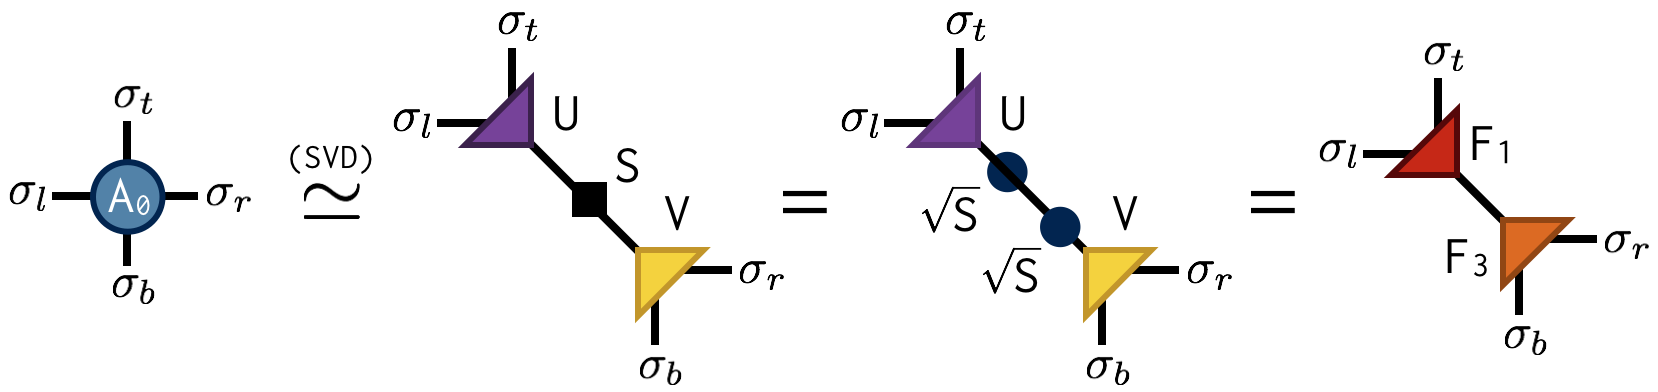
\includegraphics[width=0.8\linewidth]{images/temp/trg-factorizing-svd.png}}}
        \label{eq:trg-factorizing-svd} \\
      & \vcenter{\hbox{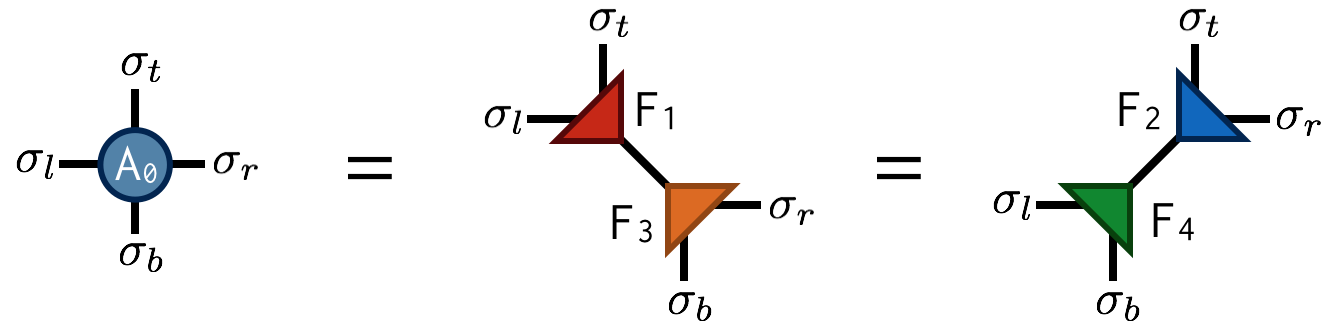
\includegraphics[width=0.65\linewidth]{images/temp/trg-factorizing.png}}}
    \end{align}
    在做 SVD 时需要对奇异值进行截断,即只保留 $\chi$ 个最大奇异值,这样可以保证 TRG 的计算开销始终在可控范围内。

  \item 把得到的三角形张量缩并为新的张量单元 $A^{(1)}$:
    \begin{equation}
      \vcenter{\hbox{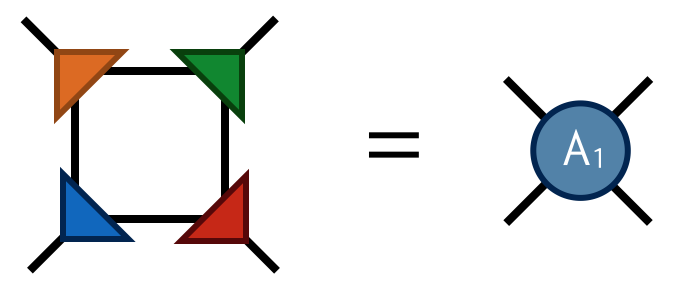
\includegraphics[width=0.35\linewidth]{images/temp/trg-group.png}}}
    \end{equation}
    此时的张量网络相当于旋转了 $45^\circ$,而总的张量数目减少了一半。

  \item 重复以上步骤,直至收敛到不动点张量。

  \item 对最终得到的不动点张量进行求迹操作即可得到配分函数 $Z$:
    \begin{equation}
      Z = \sum_{i,j} A^{(N)}_{ijij}
        = \vcenter{\hbox{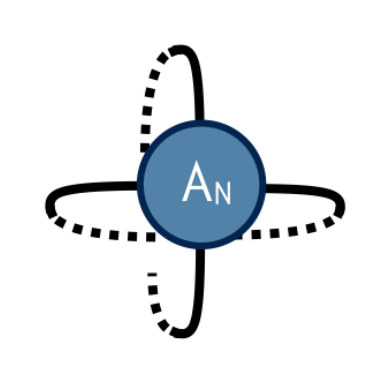
\includegraphics[width=2cm]{images/temp/trg-double-trace.png}}}
      \label{eq:trg-partition-function}
    \end{equation}
\end{enumerate}

在实际计算中直接对 $A^{(n)}$ 进行缩并会很快使数值溢出。一种常用的技术是在每一步中对 $A^{(n)}$ 进行归一化,即令其 Frobenius 范数
\begin{equation}
  \bigl| A^{(n)} \bigr|_{\mathrm{F}} = \left( \sum_{i,j,k,l} A^{(n)}_{ijkl} \right)^{1/2} = 1,
\end{equation}
并记录每步所得的范数。最终的配分函数就相当于不动点张量 $A^{(N)}$ 与这些范数的乘积。

\begin{figure}[htb]
  \centering
  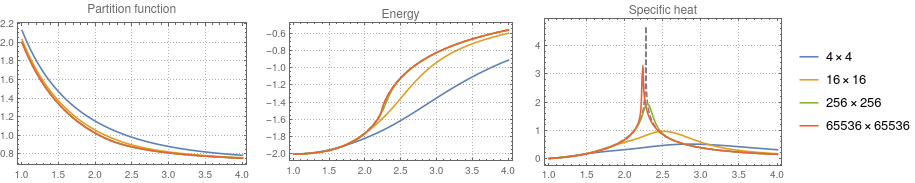
\includegraphics[width=\textwidth]{images/temp/trg-ising.png}
  \caption[利用 TRG 算法计算得到的二维 Ising 模型的各物理量]{利用 TRG 算法计算得到的二维 Ising 模型的配分函数、能量及热容。可以发现在临界点处 TRG 的计算结果与精确值(用虚线标记)有一定差异。}
  \label{fig:trg-ising}
\end{figure}

\subsection{张量网络重整化}

TRG 算法对于临界的格点模型效果并不好。这主要是由于临界系统中存在长程关联,纠缠熵
\begin{equation}
  S = -\tr(\rho\log\rho)
\end{equation}
会随着系统尺寸以对数级增长,然而通过 SVD 给出的张量分解并不能很好地保留这些信息。

如图~\ref{fig:tnr} 所示,TRG 的一种改进算法称为\emph{张量网络重整化} (tensor network renormalization, TNR)\cite{evenbly2015tensor1,evenbly2017algorithms},它借鉴了 MERA 的思想,同样使用解纠缠子 (disentangler) 和等距子 (isometry) 张量单元来实现粗粒近似。它们的具体取值可以通过最小化截断误差\cite{evenbly2015tensor1}
\begin{equation}
  \delta = \vcenter{\hbox{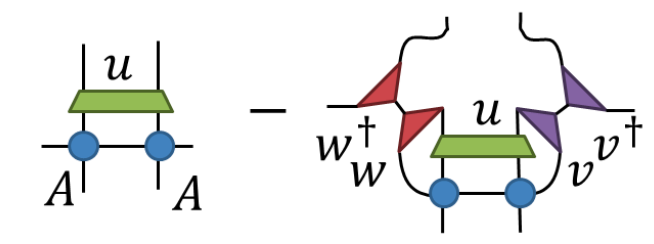
\includegraphics[width=6cm]{images/temp/tnr-truncation-error.png}}}
\end{equation}
来获得。利用角双线 (corner double line, CDL) 张量的方法可以证明\cite{evenbly2015tensor1,hauru2018renormalization},TNR 算法中的 $u$ 和 $v$ 可以消除短程纠缠的影响,使得最终获得的不动点张量的确是标度不变的。

\begin{figure}[htb]
  \centering
  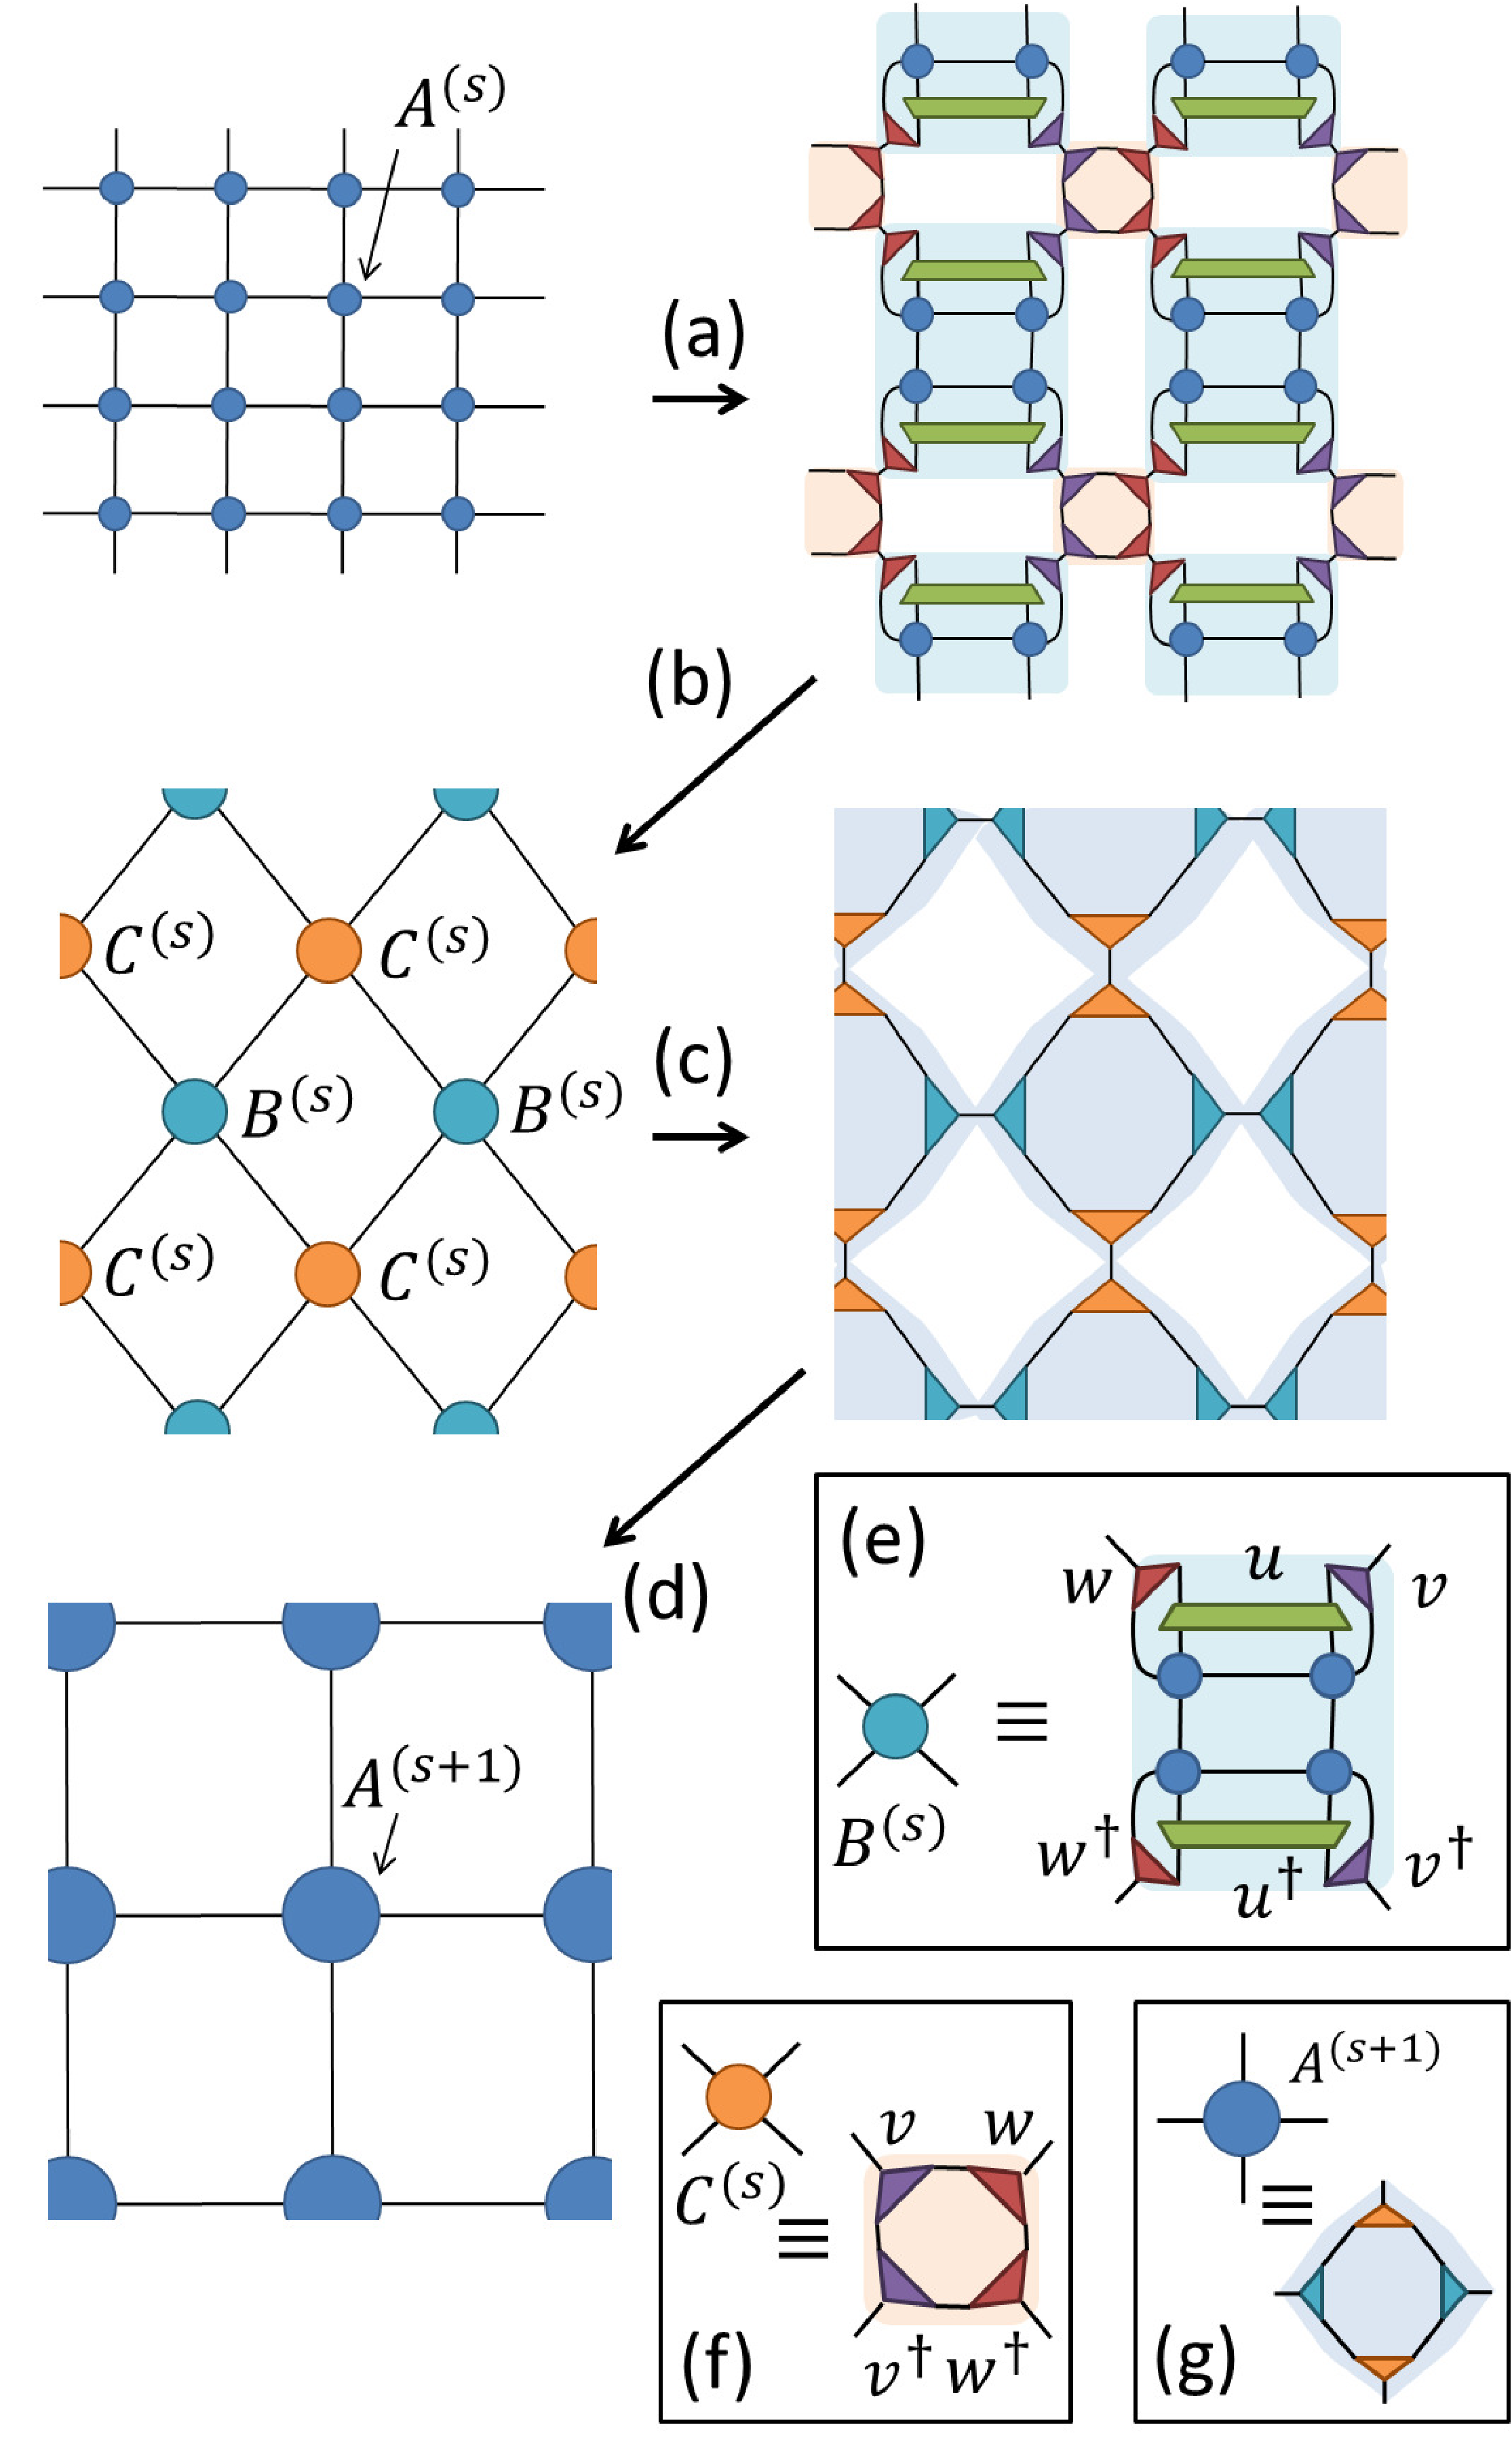
\includegraphics[width=0.6\textwidth]{images/tensor-network/tnr.pdf}
  \caption[TNR 算法]{TNR 算法。(a) 在 $2\times2$ 个 $A^{(s)}$ 张量单元之间插入解纠缠子 $u$ 和等距子 $v$。(b) 缩并得到辅助张量 $B^{(s)}$ 和 $C^{(s)}$。(c) 与 TRG 类似,利用 SVD 分解张量 $B^{(s)}$ 和 $C^{(s)}$。(d) 缩并得到新的张量单元 $A^{(s+1)}$。(e)--(g) 张量 $B^{(s)}$、$C^{(s)}$ 和 $A^{(s+1)}$ 的具体定义。图片来源:\parencite{evenbly2015tensor1}。}
  \label{fig:tnr}
\end{figure}

除了 TNR 之外,还有其他一些工作试图改进原始的 TRG 算法,如引入过滤操作以消除短程纠缠影响的\emph{张量纠缠过滤重整化} (tensor entanglement-filtering renormalization, TEFR) 算法\cite{gu2009tensor1}、基于高阶奇异值分解的\emph{高阶 TRG} (higher order TRG, HOTRG) 算法\cite{xie2012coarse}以及通过将小张量组合成环路并加以优化的\emph{环路 TNR} (loop TNR) 算法\cite{yang2017loop}等。这些方法相比 TRG 和 TNR 在精度与计算效率上各有优劣,需要根据具体问题加以权衡。

\section{具体实现}

本文后续介绍的算法主要使用 Python 语言实现,其中的张量运算则利用 NumPy\cite{harris2020array}、SciPy\cite{virtanen2020scipy}编写。它们提供了高效的张量缩并、变形以及 SVD、特征值求解等算法,并且还能通过线性算符 (linear operator) 的方法处理较大规模的稀疏矩阵与张量。此外,在硬件支持的情况下,还可以借助 GPU 甚至 TPU\cite{ganahl2023density}进一步加速计算过程。

近年来,人们使用多种语言编写了各类张量网络程序包,例如基于 MATLAB 的 NCON\cite{pfeifer2014ncon},基于 Python 的 TeNPy\cite{hauschild2018efficient}、TensorNetwork\cite{roberts2019tensornetwork}以及基于 Julia 的 TensorOperations.jl\cite{jutho2023tensoroperations}等。特别值得注意的是基于 C++ 和 Julia 实现的 ITensor\cite{fishman2022itensor}包,它能够根据指标本身的性质自动完成张量缩并,无需手动选择求和指标。文献 \parencite{psarras2021landscape} 对这些程序包的功能和特点进行了总结和比较。

在处理较大的系统时,张量缩并往往会成为计算瓶颈。为此人们提出了一系列优化方案\cite{pfeifer2014faster,evenbly2014improving},以寻找最优的缩并路径。NCON、opt\_einsum\cite{daniel2018opteinsum}等程序包中均给出了实现。

\section{本章小结}

本章主要通过图形方式介绍了张量网络方法,其中重要的运算包括张量缩并和基于 SVD 的张量分解等。我们着重讨论了一维和二维下两类张量网络算法,分别以矩阵乘积态 (MPS) 和张量重整化群 (TRG) 为代表。对于 MPS 而言,密度矩阵重整化群 (DMRG) 算法可以用来获得基态,而无限时间演化块消减 (iTEBD) 算法则可以用来处理波函数的时间演化。TRG 主要用来计算二维格点系统的配分函数,其推广张量网络重整化 (TNR) 算法可以消除短程纠缠的影响,从而能够更准确地模拟临界系统。最后,我们还简要介绍了一些常用的张量网络程序包。

\chapter{基于奇异关联子的弦网模型基态构建}

\tikzset{x=1em, y=1em, node font=\footnotesize}
\newcommand{\Vertex}[3]{
  \begin{tikzpicture}[baseline=0, thick]
    \draw (0,0) -- (90:1)  node [above] {$#1$}
          (0,0) -- (210:1) node [left]  {$#2$}
          (0,0) -- (330:1) node [right] {$#3$};
  \end{tikzpicture}
}

\section{弦网模型基态的张量网络表示}

接下来我们来给出弦网模型的基态表示\cite{gu2009tensor2,buerschaper2009explicit}。由于弦网模型的 Hamilton 量
\begin{equation}
  H = -\sum_v A_v - \sum_p B_p
\end{equation}
是严格可解的,即可以表示成一系列相互对易的投影算符之和,因而它的基态可以通过这些投影算符的本征子空间给出。式中,电荷算符 $A_v$ 指定了每个顶点处的融合规则:
\begin{equation}
  A_v \Biggl| \Vertex ijk \Biggr\rangle = \delta_{ijk} \Biggl| \Vertex ijk \Biggr\rangle, \quad
  \delta_{ijk} = \begin{cases}
    1, & \text{if $(i,j,k)$ is allowed to fuse;} \\
    0, & \text{otherwise;}
  \end{cases}
\end{equation}
磁通量算符 $B_p$ 定义为
\begin{equation}
  B_p = \sum_{s=0}^N \frac{d_s}{D} B_p^s,
\end{equation}
其中
\begin{equation}
  D = \sum_s d_s^2
\end{equation}
是总量子维数,而 $B_p^s$ 则可以图形化地视为能在方块 $p$ 处生成一个孤立环路的算符[具体定义见 \eqref{eq:string-net-bp} 式]。

于是弦网模型的基态波函数 $\ket{\psi_0}$ 可以通过在真空态 $\ket{\varnothing}$ 上作用全部的 $B_p$ 算符得到。如上所言,每个 $B_p$ 算符都是一个方块内部由对象 $R$ 构成的环路,而
\begin{equation}
  \tikz [baseline=0, very thick, draw=MaterialRed]
    \draw (0,-1) node [left] {$R$} -- (0,1.5);
  \enspace = \sum_i \frac{d_i}{D}
  \tikz [baseline=0, thick]
    \draw (0,-1) node [left] {$i$} -- (0,1.5);
\end{equation}
则是任意子按量子维数的加权叠加。因此有
\begin{equation}
  \newcommand{\VirutalLoop}{
    \draw [thick, dotted]
      (0,0) -- ++(330:1) -- ++( 30:1) -- ++( 90:1) -- ++(150:1) -- ++(210:1)
      (0,0) -- ++( 90:1) -- ++(150:1) -- ++(210:1) -- ++(270:1) -- ++(330:1)
      (0,0) -- ++(210:1) -- ++(270:1) -- ++(330:1) -- ++( 30:1) -- ++( 90:1);
  }
  \ket{\psi_0} = \prod_p B_p \ket{\varnothing} = \prod_p B_p \,
  \Biggl| \,
  \tikz [baseline=-0.3em] \VirutalLoop;
  \, \Biggr\rangle = \Biggl| \,
  \begin{tikzpicture}[baseline=-0.3em]
    \VirutalLoop;
    \draw [very thick, draw=MaterialRed]
      ( 30:1) circle [radius=0.55]
      (150:1) circle [radius=0.55]
      (270:1) circle [radius=0.55];
  \end{tikzpicture}
  \, \Biggr\rangle.
\end{equation}

为了给出 $\ket{\psi_0}$ 一种\emph{对称化}的张量网络表示,我们必须从一开始就同等对待六边形的每个边以保持对称性。需要指出的是,文献 \parencite{buerschaper2009explicit} 中通过引入奇偶子格点来构造张量网络的手段不能很好地保留旋转对称性。这里,我们需将权重(量子维数)$d_i$ 平均分配到 $R$ 环路的六个边上,使得它们在互相连接时也有良好定义:
\begin{equation}
  \newcommand{\VirutalHexagon}{
    \draw [thick, dotted]
      (30:1.2) -- (90:1.2) -- (150:1.2) -- (210:1.2) -- (270:1.2) -- (330:1.2) -- cycle;
  }
  \begin{aligned}
    % 1 segment
    \begin{tikzpicture}[baseline=-0.2em]
      \VirutalHexagon;
      \draw [very thick, draw=MaterialRed] (-30:0.8) -- (30:0.8);
    \end{tikzpicture}
    \enspace &= \sum_i \biggl( \frac{d_i}{D} \biggr)^{1/6} \enspace
    \begin{tikzpicture}[baseline=-0.2em]
      \VirutalHexagon;
      \draw [thick] (-30:0.8) node [left] {$i$} -- (30:0.8);
    \end{tikzpicture} \, , \\
    % 2 segments
    \begin{tikzpicture}[baseline=-0.2em]
      \VirutalHexagon;
      \draw [very thick, draw=MaterialRed] (-30:0.8) -- (30:0.8) -- (90:0.8);
    \end{tikzpicture}
    \enspace &= \sum_i \biggl( \frac{d_i}{D} \biggr)^{1/3} \enspace
    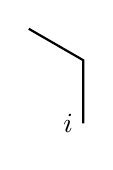
\begin{tikzpicture}[baseline=-0.2em]
      \VirutalHexagon;
      \draw [thick] (-30:0.8) node [left] {$i$} -- (30:0.8) -- (90:0.8);
    \end{tikzpicture} \, , \\
    % Loop
    \begin{tikzpicture}[baseline=-0.2em]
      \VirutalHexagon;
      \draw [very thick, draw=MaterialRed] (0,0) circle [radius=0.7];
    \end{tikzpicture}
    \enspace &= \sum_i \frac{d_i}{D} \enspace
    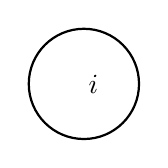
\begin{tikzpicture}[baseline=-0.2em]
      \VirutalHexagon;
      \draw [thick] (0,0) circle [radius=0.7] node [right=-0.2em] {$i$};
    \end{tikzpicture} \, .
  \end{aligned}
\end{equation}
对于邻接的六边形,我们可以在两个相邻的 $R$ 环路间执行 $F$ 移动:
\begin{align}
  \begin{tikzpicture}[baseline=-0.2em]
    \draw [thick, dotted]
      (30:1.2) -- (90:1.2) -- (150:1.2) -- (210:1.2) -- (270:1.2) -- (330:1.2)
      -- ++(-30:1.2) -- ++(30:1.2) -- ++(90:1.2) -- ++(150:1.2) -- ++(210:1.2) -- ++(270:1.2);
    \draw [very thick, draw=MaterialRed]
      (-30:0.8) -- ++(90:0.8)
      (-30:1.2) ++ (30:0.4) -- ++(90:0.8);
  \end{tikzpicture}
  \enspace &= \sum_{i,j} \biggl( \frac{d_i d_j}{D^2} \biggr)^{1/6} \enspace
  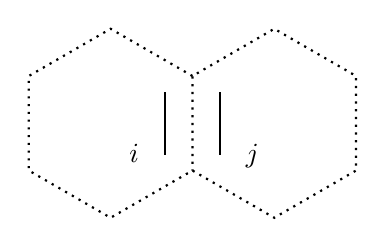
\begin{tikzpicture}[baseline=-0.2em]
    \draw [thick, dotted]
      (30:1.2) -- (90:1.2) -- (150:1.2) -- (210:1.2) -- (270:1.2) -- (330:1.2)
      -- ++(-30:1.2) -- ++(30:1.2) -- ++(90:1.2) -- ++(150:1.2) -- ++(210:1.2) -- ++(270:1.2);
    \draw [thick]
      (-30:0.8) -- ++(90:0.8)
      (-30:1.2) ++ (30:1.2-0.8) -- ++(90:0.8)
      (0.3,-0.5) node [anchor=base] {$i$}
      (1.8,-0.5) node [anchor=base] {$j$};
  \end{tikzpicture}
  \notag \\
  &= \sum_{i,j} \biggl( \frac{d_i d_j}{D^2} \biggr)^{1/6} \sum_k \sqrt{\frac{d_k}{d_i d_j}} \enspace
  \tikz [thick, baseline=-0.2em]
    \draw (90:0.6) -- +(150:1.2) node [above] {$i$} -- +(0,0) -- +(30:1.2) node [above] {$j$}
          +(0,0) -- (-90:0.6)
          +(0,0) -- +(-150:1.2) node [below] {$i$} -- +(0,0) -- +(-30:1.2) node [below] {$j$}
          (0,0) node [right] {$k$};
  \notag \\
  &= \sum_{i,j,k} \bigl( D d_i d_j \bigr)^{-1/6} d_k^{1/4} \enspace
  \begin{tikzpicture}[thick, baseline=-0.5em]
    \draw [draw=MaterialIndigo]
      (0,0) -- (270:1.2) node [below] {$k$};
    \draw [draw=MaterialPurple]
      (150:1.2) node [above=0.4, anchor=base] {$i$} -- (0,0) --
      ( 30:1.2) node [above=0.4, anchor=base] {$j$};
  \end{tikzpicture}
  \cdot \bigl( D d_i d_j \bigr)^{-1/6} d_k^{1/4} \enspace
  \begin{tikzpicture}[thick, baseline=-0.2em]
    \draw [draw=MaterialIndigo]
      (0,0) -- ( 90:1.2) node [above] {$k$};
    \draw [draw=MaterialPurple]
      (210:1.2) node [below] {$i$} -- (0,0) --
      (-30:1.2) node [below] {$j$};
  \end{tikzpicture} \, .
\end{align}
此处蓝线和紫线分别代表 $d^{-1/6}$ 和 $d^{1/4}$ 的因子。于是 $\ket{\psi_0}$ 中的每个顶点可以写成
\begin{align}
  \text{[TODO]}
\end{align}

% TODO:
在对所有的 $R$ 环路执行 $F$ 移动之后,$\ket{\psi_0}$ 现在可以表示为
\begin{equation}
  \ket{\psi_0} = ...
\end{equation}
它可以通过对位于顶点处的局域构建块进行缩并得到,并且可以用任意子基表示为
\begin{equation}
  ...
\end{equation}
这样我们就获得了六边形网格中三角形张量的对称形式:
\begin{align}
  \text{[diagram]}
  &= (d_i d_j d_k)^{-\frac14} (d_\alpha d_\beta d_\gamma)^{-\frac13} \text{[tetrahedron]} \notag \\
  &= (d_\alpha d_\beta d_\gamma)^{\frac16} (d_i d_j d_k)^{-\frac14} (d_\alpha d_\beta d_\gamma)^{-\frac12} \text{[tetrahedron]}
  \label{eq:unit-of-string-net-honeycomb}
\end{align}
对于更一般的情形,因子 $1/6$ 需要根据闭合环路中每条边的贡献进行修正。此外,我们还需要为 $B_p$ 添加额外的 $D^{-2}$ 系数,以使得 $B_p^2=B_p$。在任意三价图(每个顶点与三条边相连)中,归一化的三角形张量可以写成
\begin{equation}
  \text{[diagram]}
  = D^{-2 (1/n_\alpha + 1/n_\beta + 1/n_\gamma)}
    \bigl( d_\alpha^{1/n_\alpha} d_\beta^{1/n_\beta} d_\gamma^{1/n_\gamma} \bigr)
    (d_i d_j d_k)^{-\frac14} (d_\alpha d_\beta d_\gamma)^{-\frac12} \text{[tetrahedron]}
  \label{eq:unit-of-string-net-general}
\end{equation}
这些三角形张量每条边带有三个指标,外面的两个是\emph{虚拟指标}或\emph{辅助指标},它们会在平面内互相缩并掉;中间的一个则是\emph{物理指标},它们会伸出平面外,并且不会被缩并掉。可以看出,这实际上也是一种 PEPS 张量网络。

\begin{figure}[htb]
  \centering
  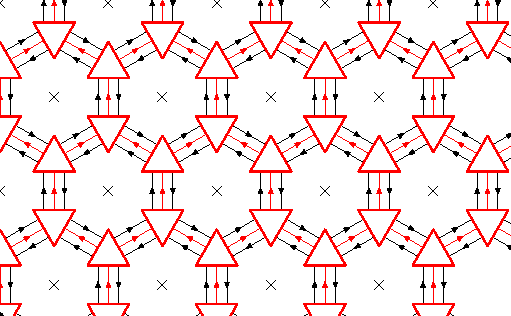
\includegraphics[width=0.6\textwidth]{images/temp/string-net-peps.pdf}
  \caption[弦网模型基态的 PEPS 张量网络表示]{弦网模型基态的 PEPS 张量网络表示。}
  \label{fig:string-net-peps}
\end{figure}

\section{奇异关联子}

\section{四面体对称性}

\section{MPO 对称性}

\section{例子}

\subsection{Fibonacci 模型}

\subsection{Ising 模型}

\chapter{Virasoro 与 Kac--Moody 代数的张量网络实现}
\label{chap:virasoro}

临界格点模型是研究\emph{共形场论} (conformal field theory, CFT) 的有力工具。有许多格点模型能够揭示出重要的 CFT 数据,而其中最基本也是最重要的一类称为\emph{最小模型} (minimal models)。它们同时也是严格可解模型,而对应的拓扑序结构可以通过融合范畴(见 \ref{sec:tensor-category-fusion-category} 节)添加进来\cite{aasen2016topological,vanhove2018mapping,aasen2020topological,huang2022numerical,vanhove2022critical}。

这些经典格点模型的配分函数通常可以表示为张量网络的形式。利用 TRG 和 TNR 等重整化算法(见 \ref{sec:tensor-network-rg} 节),可以通过控制连接维数来得到任意精度的不动点张量,从而可以高效地获取基态以及较低能级激发态(即“后代”)的对应数据。因此,这套方案有望能为分类 CFT 提供了一种数值的角度。

刻画二维 CFT 的一个重要特性是\emph{Virasoro 对称性} (Virasoro symmetry) 以及更一般情况下的\emph{Kac--Moody 对称性} (Kac--Moody symmetry),在格点模型中已有很多工作给出了它们的实现\cite{pasquier1990common,koo1994representations,milsted2017extraction,zou2018conformal,hongler2022conformal,wang2022emergence}。这些方案主要集中于构造一些作用在一维格点 Hilbert 空间上的离散算符,并对其参数取一些各向异性的极限。然而,对于一般的张量网络表示,特别是通过重整化算法得到的不动点张量,其元素往往都是数值的,没有可供展开的参数。因此使用这些方法将难以构造 Virasoro 和 Kac--Moody 生成元。对于第 \ref{chap:strange-correlator} 章中讨论的全息张量网络,这套方案也有助于在其中构造各类后代场,使得 \ref{sec:ads-cft-tensor-network} 节中体—边传播子的计算可以推广到更多的算符之中。

在本章中,我们将借用\emph{离散全纯性} (discrete holomorphicity)\cite{cardy2009discrete}的概念,给出一种构造 Virasoro 代数以及 Kac--Moody 代数的新方案\cite{wang2022virasoro,zeng2023virasoro}。对于\emph{有限尺寸效应} (finite size effect) 影响更为显著的系统(例如一些弦网模型的配分函数,见 \ref{sec:strange-correlator} 节),我们还将引入\emph{拓扑投影算符} (topological projectors),以得到符合预期精度的能动量张量以及对应的 Virasoro 生成元。

\section{二维共形场论回顾}
\label{sec:cft-review}

\emph{共形场论} (conformal field theory, CFT)\cite{belavin1984infinite,ginsparg1988applied,francesco2012conformal}的诞生源于对相变与临界现象的研究。在(二阶)相变点附近,系统应当具有\emph{标度不变性} (scaling invariance);而在二维情况下,标度不变性与共形不变性是等价的。这就意味着可以用满足\emph{共形对称性} (conformal symmetry) 的量子场论——即共形场论——来处理临界系统。

\subsection{共形对称性与能动量张量}

二维 CFT 可以用复平面上的坐标 $z$ 和 $\bar{z}$ 来描述。根据 Cauchy--Riemann 条件,共形变换 $z\to w(z)$ 和 $\bar{z}\to\bar{w}(\bar{z})$ 分别是\emph{全纯} (holomorphic) 和\emph{反全纯} (anti-holomorphic) 的,即它们只是 $z$ 和 $\bar{z}$ 的函数。在这一共形变换下,满足
\begin{equation}
  \phi(z,\bar{z}) \to \phi'(w,\bar{w}) =
  \left( \dv{w}{z} \right)^{-h} \left( \dv{\bar{w}}{\bar{z}} \right)^{-\bar{h}} \phi(z,\bar{z})
  \label{eq:quasi-primary-field}
\end{equation}
变换关系的场 $\phi$ 称为\emph{准初级场} (quasi-primary field),其中
\begin{equation}
  h = \frac12 \bigl( \Delta+s \bigr), \quad \bar{h} = \frac12 \bigl( \Delta-s \bigr)
\end{equation}
称为\emph{共形维数} (conformal dimension),而 $\Delta$ 和 $s$ 分别称为\emph{标度维数} (scaling dimension) 和\emph{自旋} (spin),它们反映了 $\phi$ 在标度和旋转变换下的性质。如果对任意的局部共形变换,式~\eqref{eq:quasi-primary-field} 都成立,则称 $\phi$ 为\emph{初级场} (primary field)。

根据 Noether 定理,(连续)对称性会与某种守恒流相对应。因而我们可以为一个一般的局部坐标变换定义\emph{能动量张量} (energy-momentum tensor),也称\emph{应力张量} (stress tensor)。在共形对称性的条件下,能动量张量 $T^{\mu\nu}$ 可以取为对称且无迹的,即只保留 $T(z)\coloneq T_{zz}(z)$ 和 $\bar{T}(\bar{z})\coloneq T_{\bar{z}\bar{z}}(\bar{z})$,同时它们也是(反)全纯函数\cite{ginsparg1988applied,cardy2010conformal,francesco2012conformal}。$T$ 和 $\bar{T}$ 的共形维数分别为 $(h_T,\bar{h}_T)=(2,0)$ 和 $(h_{\bar{T}},\bar{h}_{\bar{T}})=(0,2)$,即
\begin{equation}
  \Delta_T = \Delta_{\bar{T}} = 2, \quad s_T = 2, \quad s_{\bar{T}} = -2.
\end{equation}

对于共形维数为 $(h,\bar{h})$ 初级场 $\phi$,能动量张量与它的\emph{算子积展开} (operator product expansion, OPE) 具有如下形式:
\begin{equation}
  \begin{aligned}
    T(z) \phi(w,\bar{z}) &\sim
      \frac{h}{(z-w)^2} \phi(w,\bar{z}) + \frac{1}{z-w} \partial_w\phi(w,\bar{z}), \\
    \bar{T}(\bar{z}) \phi(w,\bar{z}) &\sim
      \frac{\bar{h}}{(\bar{z}-\bar{w})^2} \phi(w,\bar{z}) + \frac{1}{\bar{z}-\bar{w}} \partial_{\bar{w}}\phi(w,\bar{z}).
  \end{aligned}
  \label{eq:t-phi-ope}
\end{equation}
而能动量张量与自身的 OPE 则可写为
\begin{equation}
  \begin{aligned}
    T(z) T(w) &\sim
      \frac{c/2}{(z-w)^4} + \frac{2}{(z-w)^2} T(w) + \frac{1}{z-w} \partial_w T(w), \\
    \bar{T}(\bar{z}) \bar{T}(\bar{w}) &\sim
        \frac{\bar{c}/2}{(\bar{z}-\bar{w})^4}
      + \frac{2}{(\bar{z}-\bar{w})^2} \bar{T}(\bar{w})
      + \frac{1}{\bar{z}-\bar{w}} \partial_{\bar{w}}\bar{T}(\bar{w}).
  \end{aligned}
\end{equation}
其中 $(c,\bar{c})$ 称为\emph{中心荷} (central charge)。

\subsection{Virasoro 代数}

二维 CFT 可以进行\emph{径向量子化} (radial quantization),即通过
\begin{equation}
  z = \exp\left( \frac{2\pi\xi}{l} \right), \quad \xi = t+\ii x
  \label{eq:radial-quantization}
\end{equation}
将圆柱面映射到平面上,这样时间 $t$、空间 $x$ 的平移变换就相当于复平面上的缩放与旋转变换。由于等时面 $t\to-\infty$ 被映射到了复平面的坐标原点 $z=\bar{z}=0$,因而可有\emph{态—算符对应} (state-operator correspondence):
\begin{equation}
  \ket{\phi} = \lim_{t\to-\infty}\phi(x,t) \ket{0} = \lim_{z,\bar{z}\to 0} \phi(z,\bar{z}) \ket{0},
\end{equation}
这意味着每一个场算符都可以生成一个对应的量子态(波函数)。

把能动量张量进行模展开,可以得到
\begin{equation}
  \begin{aligned}
    T(z)             &= \sum_{n\in\mathbb{Z}} z^{-n-2} L_n, &\quad
    L_n              &= \frac{1}{2\pi\ii} \oint z^{n+1} T(z) \, \dd z; \\
    \bar{T}(\bar{z}) &= \sum_{n\in\mathbb{Z}} \bar{z}^{-n-2} \bar{L}_n, &\quad
    \bar{L}_n        &= \frac{1}{2\pi\ii} \oint \bar{z}^{n+1} \bar{T}(\bar{z}) \, \dd\bar{z}.
  \end{aligned}
  \label{eq:virasoro-operators}
\end{equation}
式中 $L_n$ 和 $\bar{L}_n$ 称为 \emph{Virasoro 算符} (Virasoro operators),它们构成了 \emph{Virasoro 代数} (Virasoro algebra):
\begin{equation}
  \begin{aligned}
    \bigl[ L_m, L_n \bigr]
      &= (m-n) L_{m+n} + \frac{c}{12} m \bigl( m^2-1 \bigr) \delta_{m+n,0}, \\
    \bigl[ \bar{L}_m, \bar{L}_n \bigr]
      &= (m-n) \bar{L}_{m+n} + \frac{\bar{c}}{12} m \bigl( m^2-1 \bigr) \delta_{m+n,0}, \\
    \bigl[ L_m, \bar{L}_n \bigr] &= 0.
  \end{aligned}
  \label{eq:virasoro-algebra}
\end{equation}
真空态 $\ket{0}$ 需要在全局共形变换下保持不变,这要求
\begin{equation}
  L_n \ket{0} = \bar{L}_n \ket{0} = 0, \quad n \geqslant -1.
\end{equation}
设初级场 $\phi$ 对应的态为 $\ket*{h,\bar{h}}\coloneq\phi(0,0)\ket{0}$。根据式~\eqref{eq:t-phi-ope},可知
\begin{equation}
  L_0       \ket*{h,\bar{h}} = h       \ket*{h,\bar{h}}, \quad
  \bar{L}_0 \ket*{h,\bar{h}} = \bar{h} \ket*{h,\bar{h}}, \quad
  L_n \ket*{h,\bar{h}} = \bar{L}_n \ket*{h,\bar{h}} = 0 \enspace (n > 0).
\end{equation}
代入式~\eqref{eq:virasoro-algebra} 中的对易关系,有
\begin{equation}
  \bigl[ L_0, L_{-n} \bigr] = n L_{-n}, \quad
  \bigl[ \bar{L}_0, \bar{L}_{-n} \bigr] = n \bar{L}_{-n}.
\end{equation}
可以看出 $L_{-n}\ket{0}$ 和 $\bar{L}_{-n}\ket{0}$ 分别是 $L_0$ 和 $\bar{L}_0$ 本征值为 $n$ 的本征态,因而 $L_{-n}$、$\bar{L}_{-n}$ 即可作为升算符,使得共形维数 $h$、$\bar{h}$ 增加 $n$。产生的这些态称为 $\ket*{h,\bar{h}}$ 的\emph{后代} (descendant),它们也可以通过对 $\phi$ 求导得到。

\subsection{Kac--Moody 代数}

当 CFT 具有额外的对称性时,Virasoro 代数可以推广为 \emph{Kac--Moody 代数} (Kac--Moody algebra)\cite{goddard1986kac,wang2022emergence}。考虑一个具有 $G$ 对称性的 CFT,其中 $G$ 是一个半单 Lie 群,而对应的 Lie 代数为 $\mathfrak{g}$。守恒荷 $Q^\alpha$ 可以表示为局域守恒流 $q^\alpha$ 的积分:
\begin{equation}
  Q^\alpha = \int q^\alpha(x) \, \dd{x} = \int \bigl[ J^\alpha(x) + \bar{J}^\alpha(x) \bigr] \, \dd{x}.
\end{equation}
这里我们把 $q^\alpha$ 分为了全纯部分 $J^\alpha$ 与反全纯部分 $\bar{J}^\alpha$,它们称为\emph{流算符} (current operatots),其共形维数分别为 $(1,0)$ 和 $(0,1)$,而 $\alpha=1,2,\ldots,|\mathfrak{g}|$ 标记了不同的流。仿照式~\eqref{eq:virasoro-operators} 中 Virasoro 算符的情形,我们也可以对流算符进行模展开:
\begin{equation}
  J^\alpha_n = \frac{1}{2\pi\ii} \oint z^{n+1} J^\alpha(z) \, \dd z, \quad
  \bar{J}^\alpha_n = \frac{1}{2\pi\ii} \oint \bar{z}^{n+1} \bar{J}^\alpha(\bar{z}) \, \dd\bar{z}.
\end{equation}
它们满足 Kac--Moody 代数 $\hat{\mathfrak{g}}_k$:
\begin{equation}
  \begin{aligned}
    \bigl[ J^\alpha_m, J^\beta_n \bigr]
      &= \ii \sum_\gamma f^{\alpha\beta\gamma} J^\gamma_{m+n} + km \delta^{\alpha\beta} \delta_{m+n,0}, \\
    \bigl[ \bar{J}^\alpha_m, \bar{J}^\beta_n \bigr]
      &= \ii \sum_\gamma f^{\alpha\beta\gamma} \bar{J}^\gamma_{m+n} + km \delta^{\alpha\beta} \delta_{m+n,0}, \\
    \bigl[ J^\alpha_m, \bar{J}^\beta_n \bigr] &= 0,
  \end{aligned}
  \label{eq:kac-moody-algebra}
\end{equation}
其中 $f^{\alpha\beta\gamma}$ 是 Lie 代数 $\mathfrak{g}$ 的结构常数,$k$ 是\emph{能级常数} (level constant)。令 $n=m=0$,即得到通常 Lie 代数的对易关系
\begin{equation}
  \bigl[ J^\alpha_0, J^\beta_0 \bigr] = f^{\alpha\beta\gamma} J^\gamma_0.
\end{equation}

Virasoro 与 Kac--Moody 生成元之间也满足对易关系:
\begin{equation}
  \bigl[ L_m, J^\alpha_n \bigr] = -n J^\alpha_{m+n}, \quad
  \bigl[ \bar{L}_m, \bar{J}^\alpha_n \bigr] = -n \bar{J}^\alpha_{m+n}.
\end{equation}
这说明 $J^\alpha$ 和 $\bar{J}^\alpha$ 确实是共形维数 $(1,0)$、$(0,1)$ 的 Virasoro 初级场。而令 $m=0$,则可以看出 $J^\alpha_n$、$\bar{J}^\alpha_n$ 与 Virasoro 生成元一样可作为升降算符,使得 $h$、$\bar{h}$ 改变 $n$。当 $n=0$ 时,Virasoro 与 Kac--Moody 生成元对易:
\begin{equation}
  \bigl[ L_0, J^\alpha_0 \bigr] = \bigl[ \bar{L}_0, \bar{J}^\alpha_0 \bigr] = 0,
\end{equation}
因而它们具有相同的本征态。这也进一步印证了 $J^\alpha$ 和 $\bar{J}^\alpha$ 确实是守恒流。

\subsection{环面配分函数}

将圆柱面的 $t\to\pm\infty$ 等时面“粘”在一起便可得到环面。环面的几何由参数 $\tau=\tau_1+\ii\tau_2$ 表示,它需要在变换
\begin{equation}
  \tau \to \frac{a\tau+b}{c\tau+d}, \quad \begin{pmatrix} a & b \\ c & d \end{pmatrix} \in PSL(2,\mathbb{Z})
\end{equation}
下保持不变,其中 $PSL(2,\mathbb{Z})=SL(2,\mathbb{Z})/\mathbb{Z}_2$ 称为\emph{模群} (modular group)。此时配分函数可以写为\cite{cardy1986operator,francesco2012conformal}
\begin{align}
  Z &= \tr \Bigl[ \exp \bigl( -2\pi\tau_2 H \bigr) \exp \bigl( 2\pi\ii\tau_1 P \bigr) \Bigr] \notag \\
    &= \tr \Bigl[
         \exp \Bigl( -2\pi   \tau_2 \Bigl( L_0 + \bar{L}_0 - \frac{c}{12} \Bigr) \Bigr)
         \exp \Bigl(  2\pi\ii\tau_1 \bigl( L_0 - \bar{L}_0 \bigr) \Bigr)
       \Bigr].
\end{align}
其中 $H$ 和 $P$ 分别是 Hamilton 算符和动量算符:
\begin{equation}
% TODO: why c/12; how about c-bar
  H = L_0 + \bar{L}_0 - \frac{c}{12}, \quad P = \ii \bigl( L_0 - \bar{L}_0 \bigr),
\end{equation}
而 $c$ 是中心荷。设场 $\phi_\alpha$ 的共形维数为 $(h_\alpha,\bar{h}_\alpha)$,由 Virasoro 代数可知
\begin{align}
  Z &= \sum_\alpha \exp \Bigl[
         - 2\pi   \tau_2 \Bigl( h_0 + \bar{h}_0 - \frac{c}{12} \Bigr)
         + 2\pi\ii\tau_1 \bigl( h_0 - \bar{h}_0 \bigr)
       \Bigr] \notag \\
    &= \sum_\alpha \exp \Bigl[
         - 2\pi   \tau_2 \Bigl(\Delta_\alpha - \frac{c}{12} \Bigr)
         + 2\pi\ii\tau_1 s_\alpha
       \Bigr],
  \label{eq:torus-partition-function}
\end{align}
其中 $\Delta_\alpha$ 和 $s_\alpha$ 分别是场 $\phi_\alpha$ 的标度维数和自旋。

\subsection{格点近似}
\label{subsec:lattice-approximation}

% TODO:
% 临界格点模型的配分函数可以通过张量网络来描述。以只包含最邻近相互作用的模型为例,其配分函数为
% \begin{equation}
%   Z = \sum_{\sigma_i} \prod_{\langle i,j \rangle} \ee^{-\beta E_{ij}}.
% \end{equation}
% 考虑一个方块附近的四个自由度 $\sigma_i$、$\sigma_j$、$\sigma_k$、$\sigma_l$,令
% \begin{equation}
%   A_{ijkl} = \ee^{-\beta (H_{ij}+H_{jk}+H_{kl}+H_{li})},
% \end{equation}
% 则 $Z$ 可以写成
% \begin{equation}
%   Z = ...
% \end{equation}
% 四个指标的张量 $A_{ijkl}$ 可以排列成一个 $m\times n$ 的网格

% 由于在二维 CFT 中存在态—算符对应,不妨先假想一个以原点为圆心的圆盘,当我们在原点插入一个算符时,圆盘边界处便会产生一个量子态。如果插入的算符是初级场或其后代,那么对应的量子态将会是缩放算符 (dilation operator) 的本征态。利用式~\eqref{eq:radial-quantization} 的逆映射
% \begin{equation}
%   \xi = \frac{l}{2\pi} \log z
% \end{equation}
% 可将复平面变为圆柱,而此时的缩放算符即为沿圆柱轴向的路径积分。

如图~\ref{fig:partition-function-tensor-network} 所示,临界格点模型的配分函数 $Z$ 可以通过张量网络来描述:
\begin{equation}
  Z = \sum_{i_n,j_n,k_n,l_n} \prod_{\alpha=1}^n A_{i_\alpha j_\alpha k_\alpha l_\alpha},
  \label{eq:partition-function-tensor-network}
\end{equation}
其中 $A_{ijkl}$ 是四个指标的张量单元。如果把这个网格的两边“粘”起来,并且只取其中一层,就得到了相应的转移矩阵。同时可以发现,如果在平面的张量网络中插入一个算符,围绕算符边界的张量可以连成一个环,而这个环和圆柱上的转移矩阵(在极限意义下)是等价的。这实际上正是式~\eqref{eq:radial-quantization} 用张量网络语言的表述。因此,转移矩阵的本征态便可用来近似描述在平面上插入的算符。

\begin{figure}[ht]
  \centering
  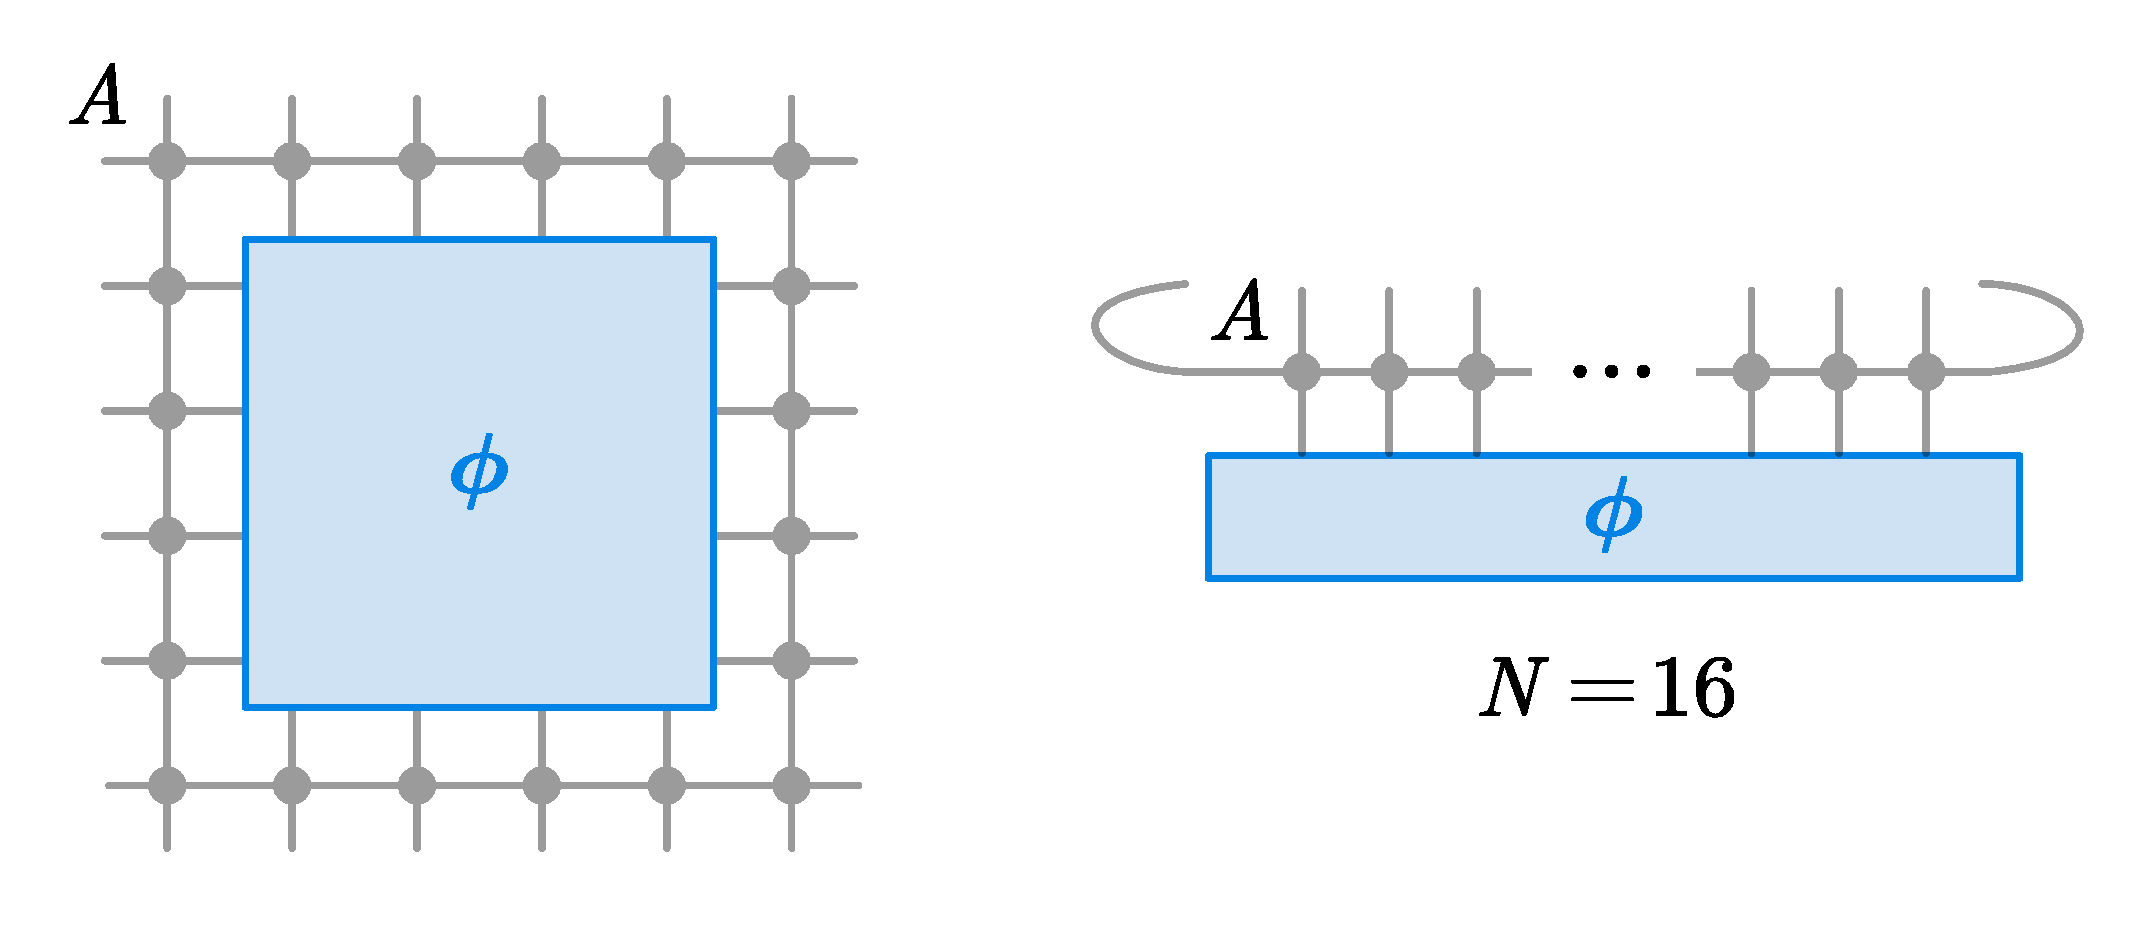
\includegraphics[width=0.6\textwidth]{images/virasoro/transfer-matrix.pdf}
  \caption[格点模型配分函数的张量网络描述]{格点模型配分函数的张量网络描述。图片来源:\parencite{wang2022virasoro}。}
  \label{fig:partition-function-tensor-network}
\end{figure}

下面我们来计算转移矩阵的本征值。考虑一个 $m\times n$ 网格上的临界格点模型,并且模型满足周期性边界条件。它的连续极限可以用一个环面上的 CFT 来描述,环面参数为 $\tau=\ii m/n$。根据式~\eqref{eq:torus-partition-function},配分函数为\cite{hauru2016topological}
\begin{equation}
  Z = \sum_\alpha \exp \Bigl[
        - 2\pi \frac mn \Bigl(\Delta_\alpha - \frac{c}{12} \Bigr)
        + mnf + \mathcal{O} \Bigl( \frac{m}{n^\gamma} \Bigr)
      \Bigr],
\end{equation}
其中 $f$ 是热力学极限下每一格点的自由能,而 $\mathcal{O}(m/n^\gamma)$ 则是有限尺寸效应带来的修正。配分函数的“一层”也就是转移矩阵:
\begin{equation}
  Z = \tr M^m,
\end{equation}
因此 $M$ 的本征值为
\begin{equation}
  \lambda_\alpha = \exp \Bigl[
        - \frac{2\pi}{n} \Bigl(\Delta_\alpha - \frac{c}{12} \Bigr)
        + nf + \mathcal{O} \Bigl( \frac{1}{n^\gamma} \Bigr)
      \Bigr].
\end{equation}
由于真空态的标度维数总是 0,我们可以据此消去自由能和有限尺寸修正:
\begin{equation}
  \Delta_\alpha = \frac{n}{2\pi} \bigl( \log\lambda_0 - \log \lambda_\alpha \bigr).
\end{equation}
而如果可以确定能动量张量,还可以利用 $\Delta_T=2$ 的性质来标定 $\Delta_\alpha$:
\begin{equation}
  \Delta_\alpha = \frac{2}{\log\lambda_0 - \log\lambda_T} \bigl( \log\lambda_0 - \log \lambda_\alpha \bigr).
  \label{eq:scaling-dimension-rescale}
\end{equation}

自旋部分可以通过引入平移算符 $P$ 来得到。在圆柱上,可以写为 $\exp(2\pi\ii P/n)$,而其本征值为 $\exp(2\pi\ii s_\alpha/n)$。在具有平移对称性的模型中,$\exp(2\pi\ii P/n)$ 和转移矩阵 $M$ 对易,因此它们可以被同时对角化。平移算符 $P$ 的张量网络表示为\cite{van2021efficient}:
\begin{equation}
  P_{i_1 i_2 \cdots i_n, \, j_1 j_2 \cdots j_n} = \tikzinput{translation-operator},
\end{equation}
即把格点平移一个单位。

\section{Virasoro 与 Kac--Moody 算符的构造}
\label{sec:virasoro-operators}

类比连续情况下的式~\eqref{eq:virasoro-operators},格点 Virasoro 算符可以表示为
\begin{equation}
  L_n       \sim \sum_{j=1}^N \ee^{ \ii j n \frac{2\pi}{N}} T(j), \quad
  \bar{L}_n \sim \sum_{j=1}^N \ee^{-\ii j n \frac{2\pi}{N}} \bar{T}(j),
  \label{eq:lattice-virasoro-operators}
\end{equation}
其中 $T(j)$ 和 $\bar{T}(j)$ 是能动量张量位于 $j$ 处的格点表示。

对于一些具体的格点模型\cite{koo1994representations,milsted2017extraction},能动量张量 $T$ 可以解析求出。然而在一般情况下,通过配分函数并不能直接得到 $T$ 的表达式。为此,我们需要利用张量网络来构造 Virasoro 算符的近似表示。

如图~\ref{fig:virasoro-construction} 所示,考虑一个以 $A_{ijkl}$ 为单元构成的一般性的张量网络,其中连接维数 $\chi_A=d$。将 $A$ 张量连成一个圆柱得到转移矩阵、与平移算符相连,再对其进行精确对角化,即可按照 \ref{subsec:lattice-approximation} 小节中介绍的方案来确定本征态 $\ket*{\phi_T}$ 或 $\ket*{\phi_{\bar{T}}}$,以及相应的能动量张量 $T$ 或 $\bar{T}$。随后,我们可以把得到的 $T$ 或 $\bar{T}$ 插回由 $A$ 构成的圆柱(即把 $j$ 位置处的 $A$ 张量用 $T$ 或 $\bar{T}$ 取代),再根据式~\eqref{eq:lattice-virasoro-operators} 乘上对应的系数 $\ee^{\pm2\pi\ii j n/N}$,这样就构造出了格点上的 Virasoro 算符 $L_n$ 或 $\bar{L}_n$。

\begin{figure}[ht]
  \centering
  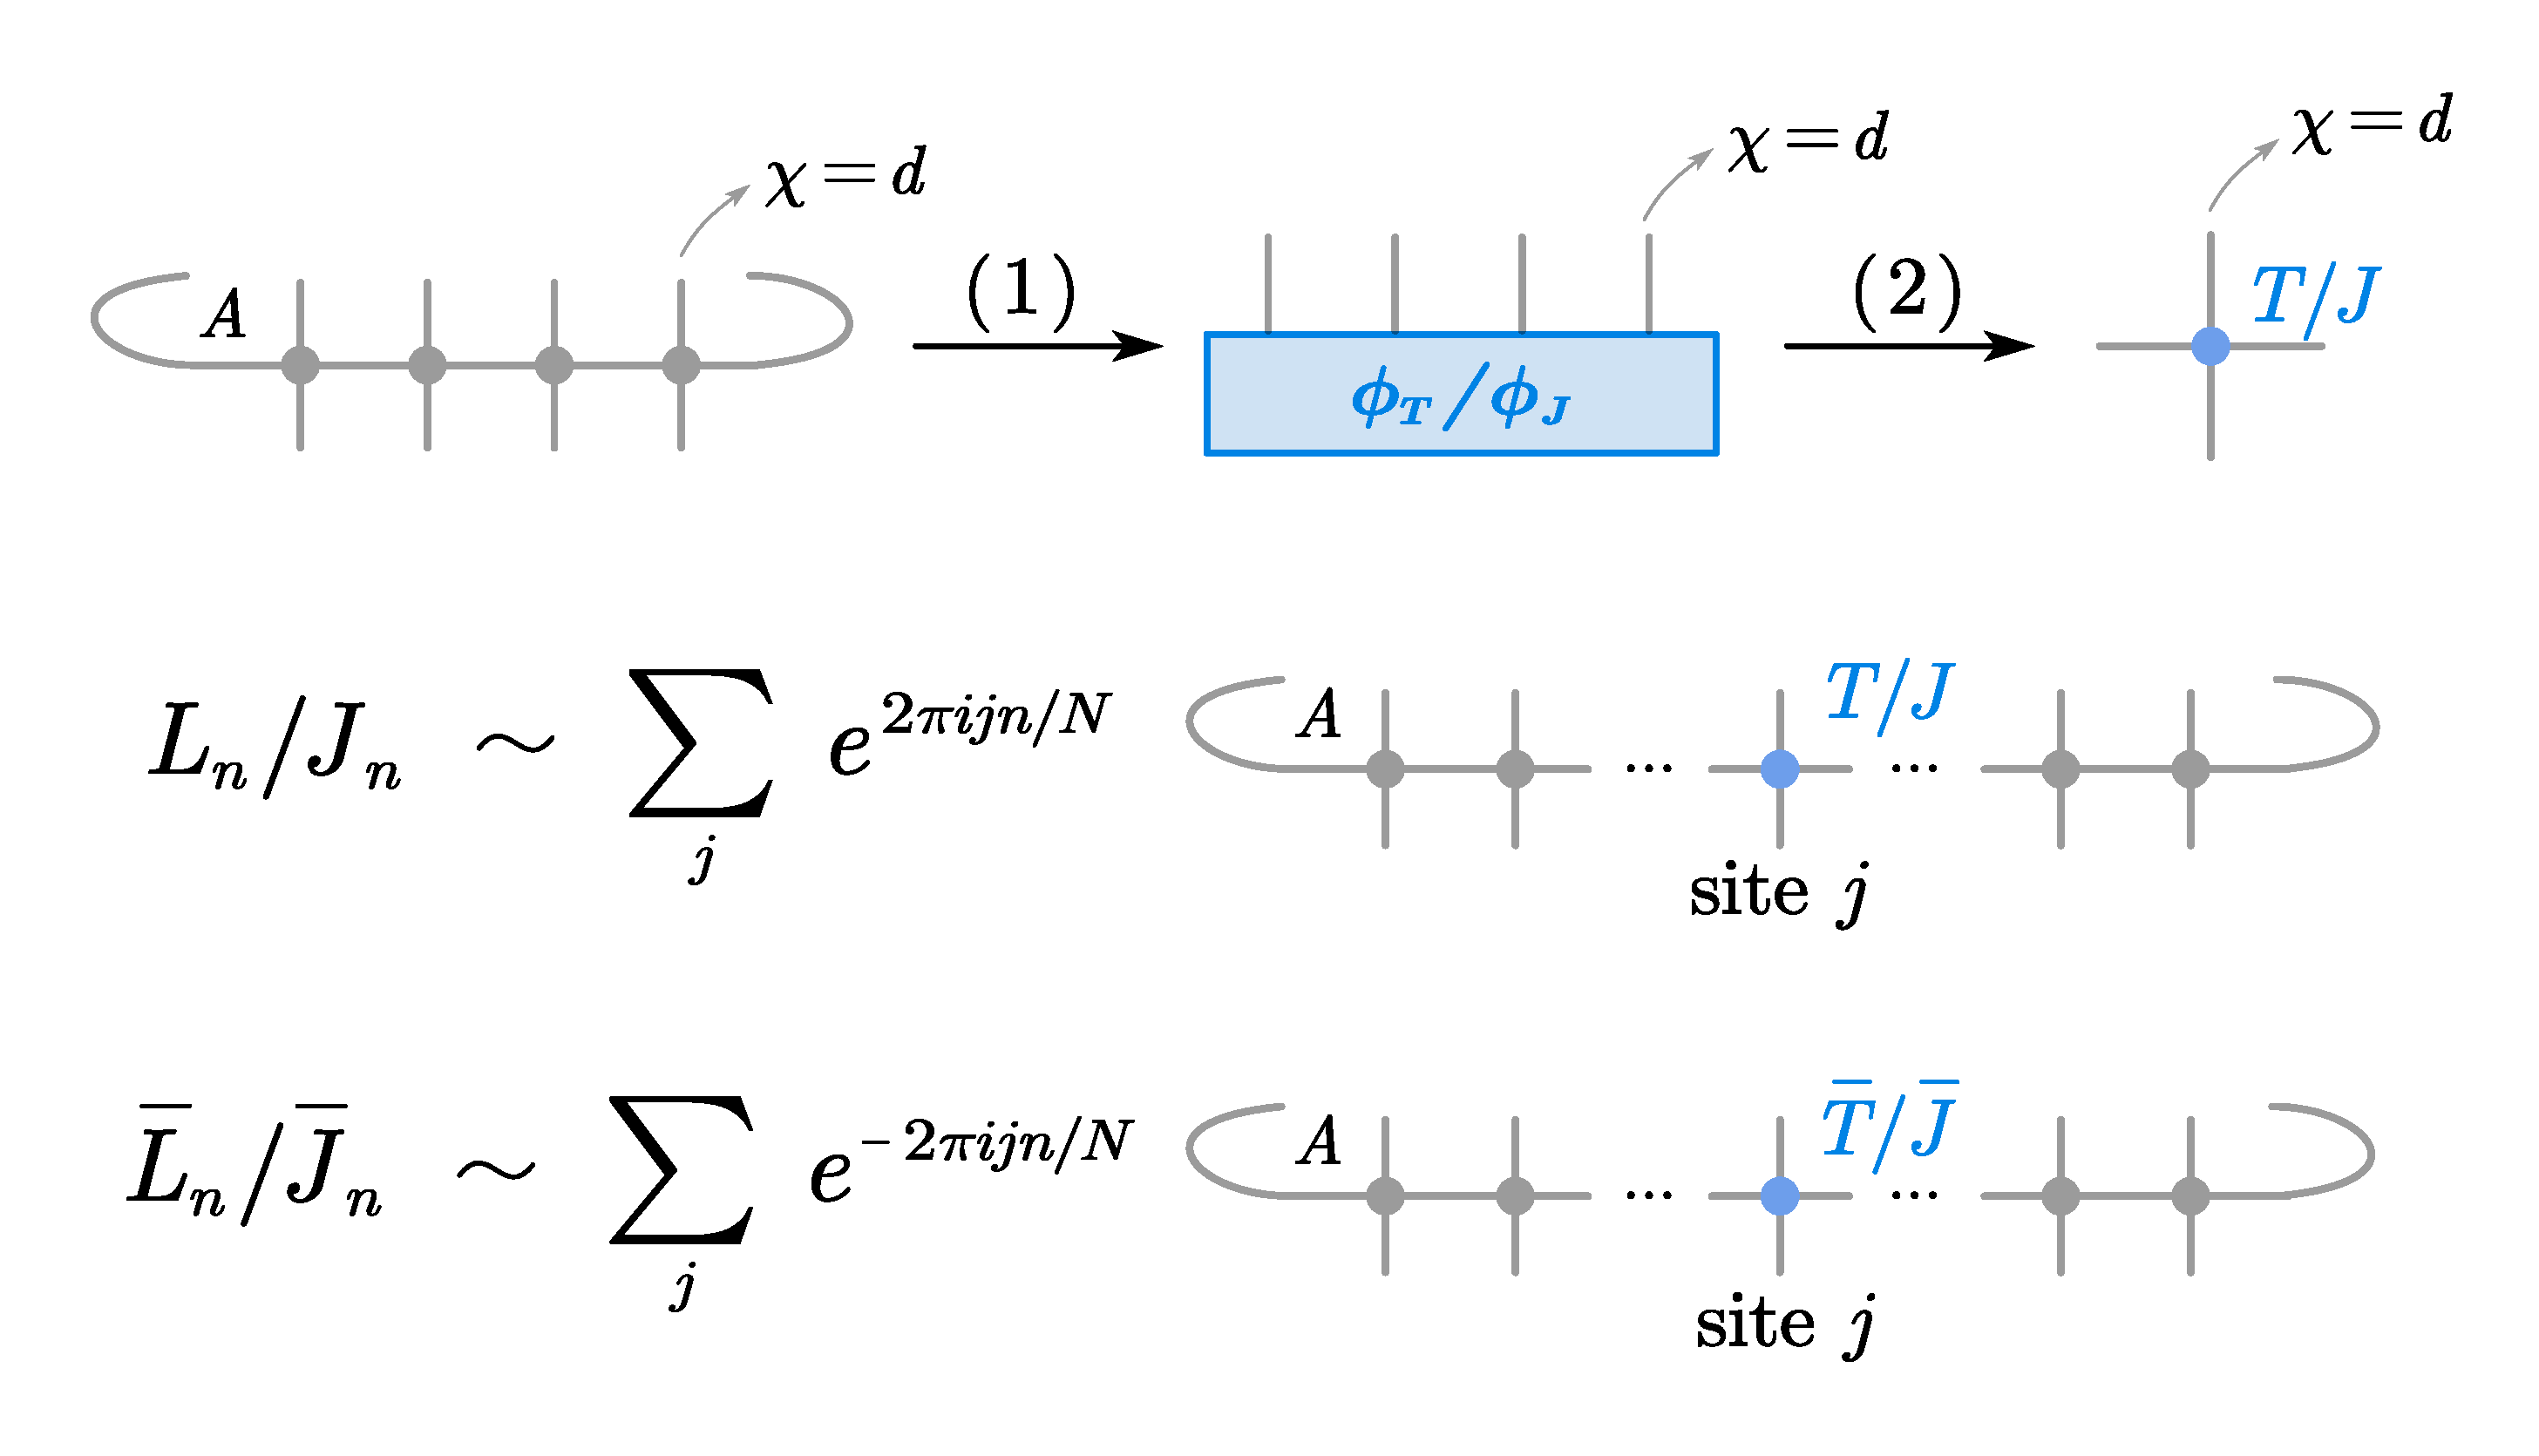
\includegraphics[width=0.8\textwidth]{images/virasoro/construction.pdf}
  \caption[能动量张量与 Virasoro 算符的构造]{在一般的张量网络中确定能动量张量 $T$,并以此来构造 Virasoro 算符[见式~\eqref{eq:lattice-virasoro-operators}]。对应于与能动量张量的本征态 $\ket*{\phi_T}$ 可以从圆柱转移矩阵中通过精确对角化得到,它被进一步变形为 4 个指标的张量 $T$,并插入到新的圆柱中,由此即可得到 Virasoro 算符 $L_n$。同样的方法也可用来构造 Kac--Moody 算符 $J_n$。图片来源:\parencite{wang2022virasoro}。}
  \label{fig:virasoro-construction}
\end{figure}

当模型具有额外对称性时,相应 CFT 中的 Virasoro 对称性可以推广为 Kac--Moody 对称性。我们可以用完全类似的方法来构造格点 Kac--Moody 算符:
\begin{equation}
  J_n       \sim \sum_{j=1}^N \ee^{ \ii j n \frac{2\pi}{N}} J(j), \quad
  \bar{J}_n \sim \sum_{j=1}^N \ee^{-\ii j n \frac{2\pi}{N}} \bar{J}(j),
\end{equation}
其中 $J(j)$ 和 $\bar{J}(j)$ 是共形维数分别为 $(1,0)$ 和 $(0,1)$ 的流算符。

\section{例子:Ising 模型}

二维正方形网格上的 Ising 模型,其配分函数为
\begin{equation}
  Z = \sum_{\{\sigma\}} \ee^{-\beta H}
    = \sum_{\{\sigma\}} \ee^{\beta \sum_{\ev{ij}} \sigma_i \sigma_j}
    = \sum_{\{\sigma\}} \prod_{\ev{ij}} \ee^{\beta \sigma_i \sigma_j}
    = \tr M^m,
\end{equation}
其中 $\sigma\in\{-1,+1\}$ 是 Ising 自旋。它可以按式~\eqref{eq:partition-function-tensor-network} 的形式用张量网络表示,对应的张量单元为
\begin{equation}
  A^{(0)}_{ijkl} = \ee^{-\beta (\sigma_i\sigma_j + \sigma_j\sigma_k + \sigma_k\sigma_l + \sigma_l\sigma_i)}.
\end{equation}
在临界点处,$\beta=\beta_{\text{c}}=\log(1+\sqrt2)/2$。转移矩阵为
\begin{equation}
    M^{i_1 i_2 \cdots i_n}_{k_1 k_2 \cdots k_n}
  = \sum_{j_1, j_2, \ldots, j_n} \prod_{\alpha=1}^n A^{(0)}_{i_\alpha j_\alpha k_\alpha j_{\alpha+1}}
  = \tikzinput{ising/cylinder}.
\end{equation}

在实际计算中,可以对张量 $A$ 进行粗粒近似以提高精度,如图~\ref{fig:virasoro-blocking} 所示。例如可将 4 个 $A$($\eqcolon A^{(0)}$)组合成一个更大的 $A^{(1)}$,也可不断重复使得 $A^{(i)}$ 逐渐接近不动点张量。在这一过程中,连接维数 $\chi_{A^{(i)}}=d^{2^i}$ 会迅速增大,因此往往还需要进行截断。实际上,这也就是利用 TRG 或 TNR 等张量网络算法\cite{levin2007tensor,evenbly2015tensor1,evenbly2017algorithms}来寻找不动点张量的操作。

\begin{figure}[ht]
  \centering
  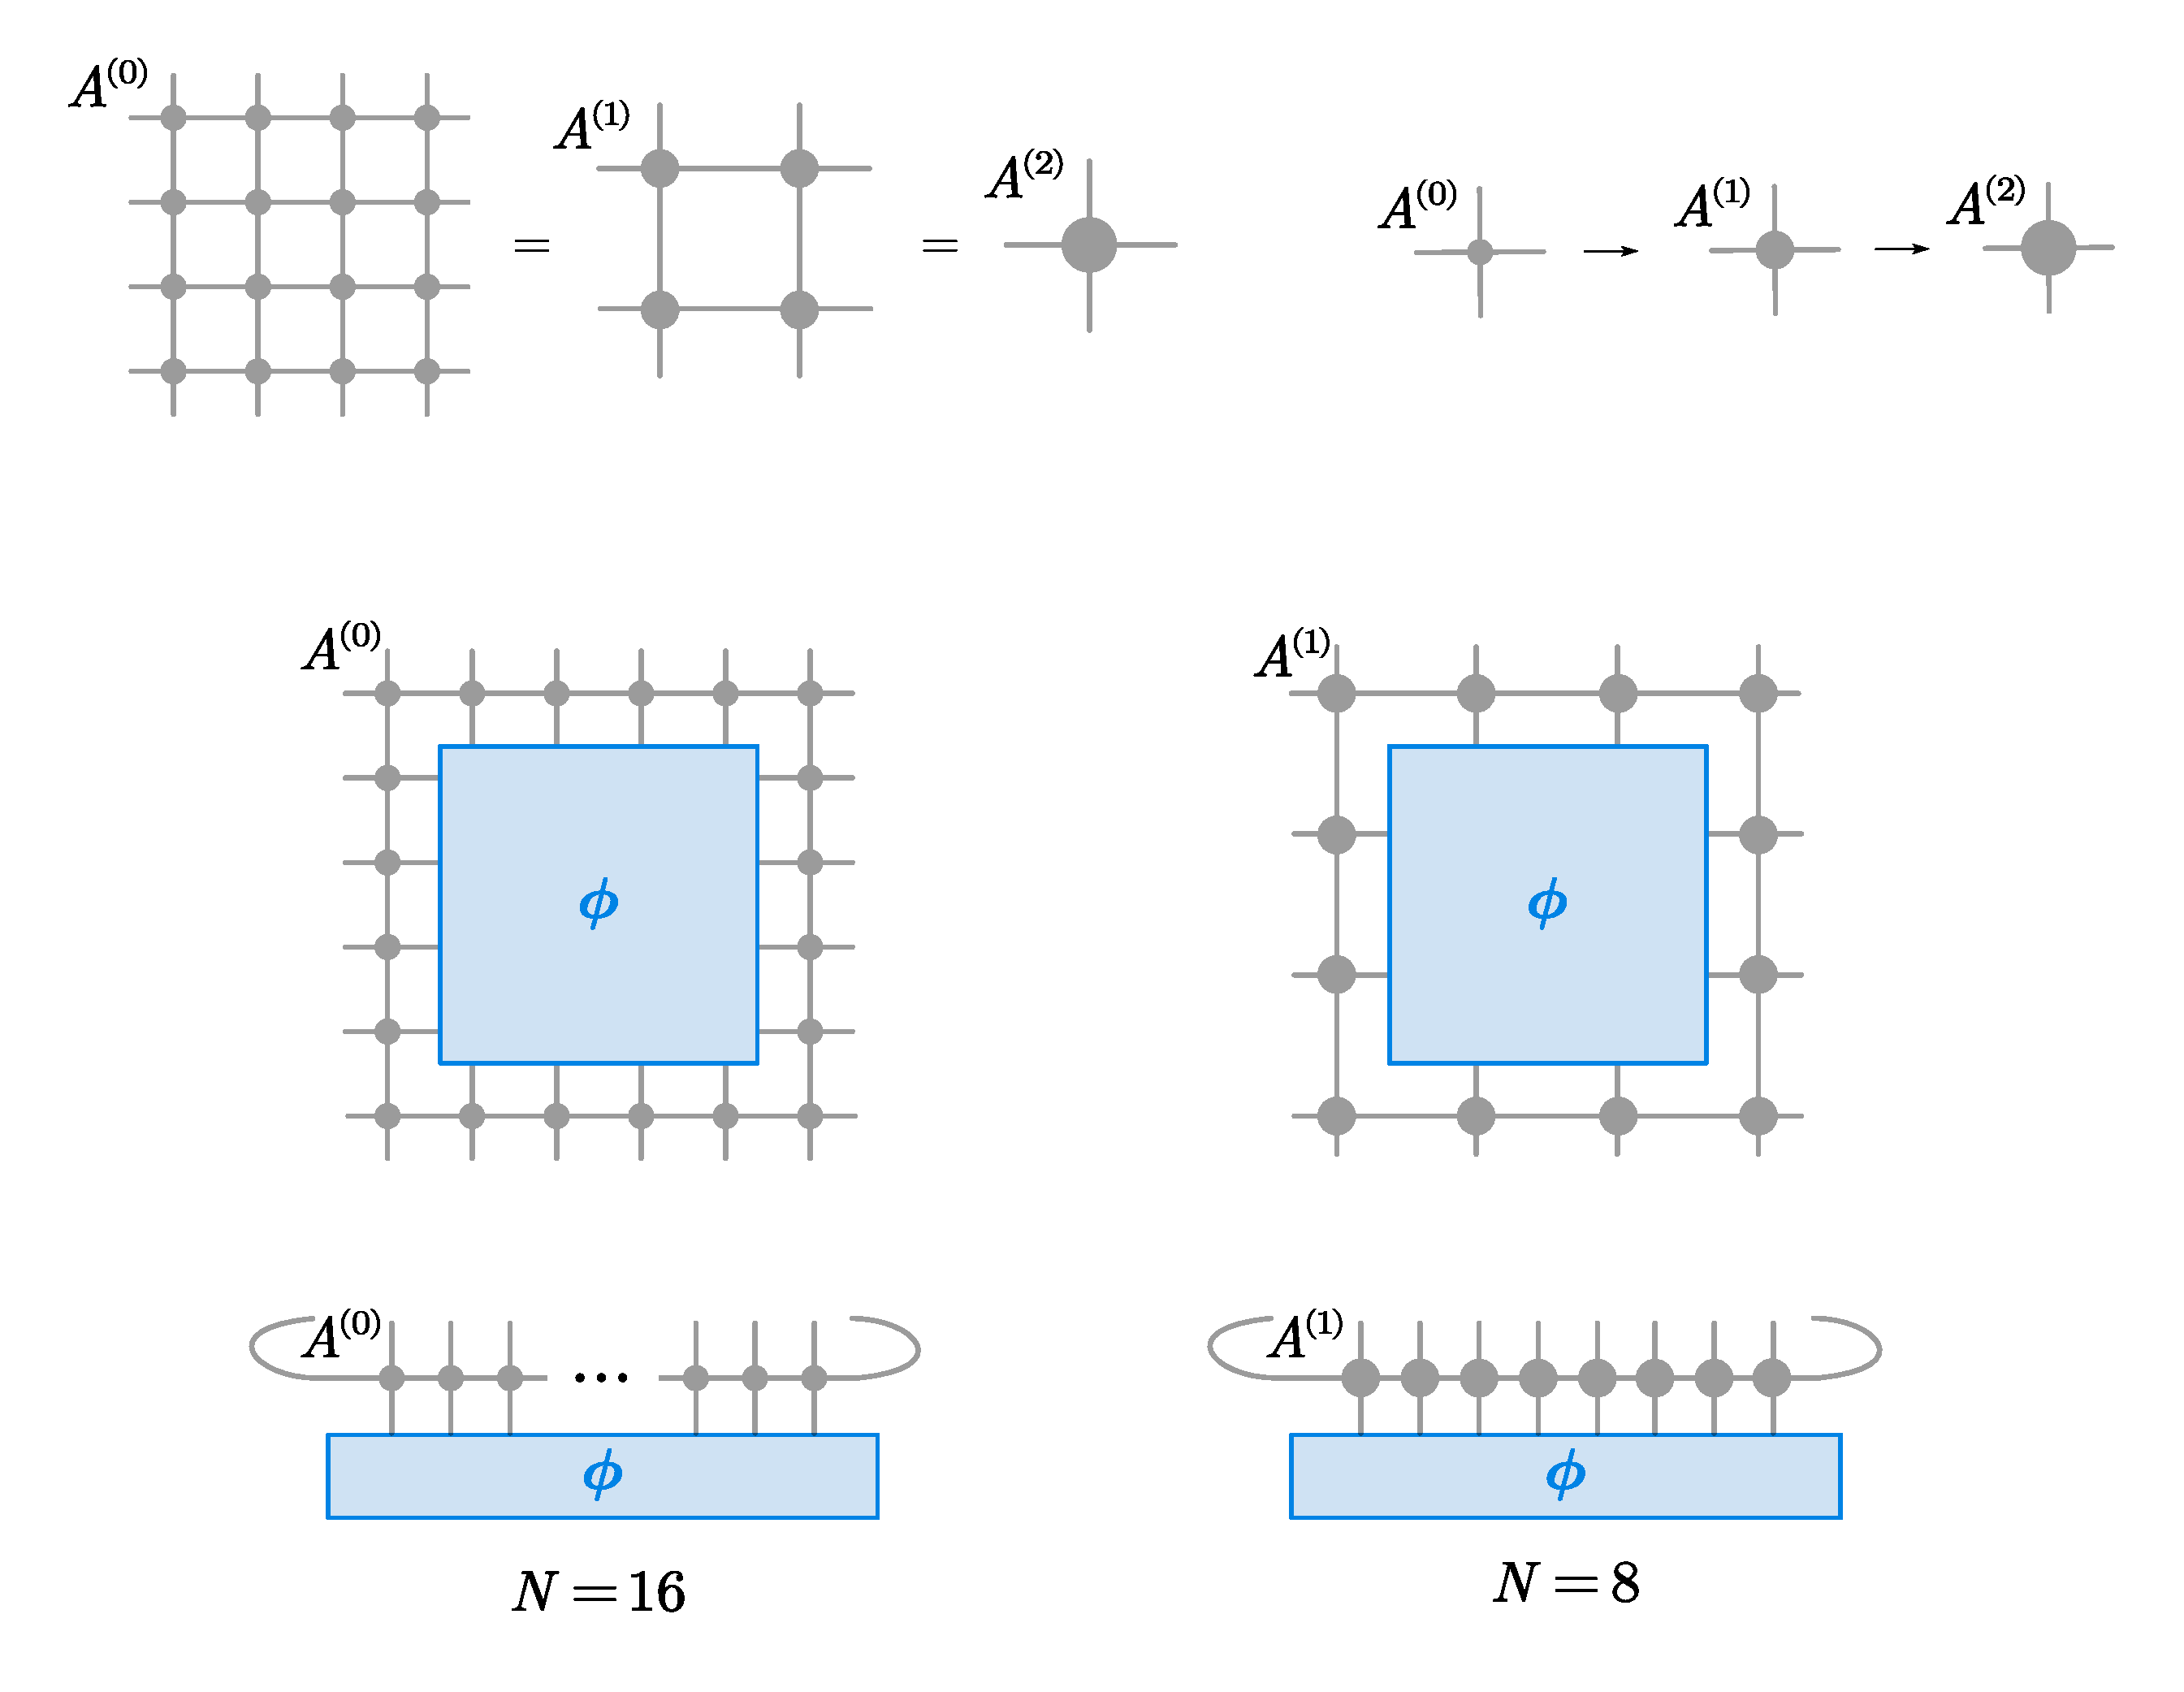
\includegraphics[width=0.9\textwidth]{images/virasoro/blocking.pdf}
  \caption[张量 $A$ 的粗粒近似]{对张量 $A$ 进行粗粒近似。上图:$2\times2\mapsto1$ 的粗粒近似操作,$A^{(s+1)}$ 可由 4 个 $A^{(s)}$ 张量缩并得到。下图:相应的算符可以等效为一个指标更少、但连接维数更大的正方形张量。图片来源:\parencite{wang2022virasoro}。}
  \label{fig:virasoro-blocking}
\end{figure}

\subsection{CFT 能谱与能动量张量}

在确定能动量张量的过程中,为了使得 $T$ 或 $\bar{T}$ 之后能被插入到圆柱中,它们必须有 4 个指标。如果使用 4 个 $A^{(0)}$ 张量组成转移矩阵,虽然得到的本征态形状满足要求,但此时 $\ket*{\phi_T}$ 和 $\ket*{\phi_{\bar{T}}}$ 将会是简并的(由于 $-2\bmod4=+2$,计算得到的自旋都是 $+2$)。因此我们将使用 $N=8$ 的转移矩阵来进行精确对角化以得到能谱数据(见图~\ref{fig:ising-spectrum}、图~\ref{fig:ising-virasoro} 和表~\ref{tab:ising-spectrum}),并从中找到标度维数 $\Delta\approx2$、自旋 $s=\pm2$ 的 $\ket*{\phi_T}$ 和 $\ket*{\phi_{\bar{T}}}$,并将它们从 8 个指标、$\chi=2$ 变形为 4 个指标、$\chi=4$ 的张量 $T$ 和 $\bar{T}$。对于 Ising 模型,此时已经可以得到较好的精度,因此在这一步中我们没有使用粗粒近似后的 $A^{(i)}$ 张量。

\begin{figure}[ht]
  \centering
  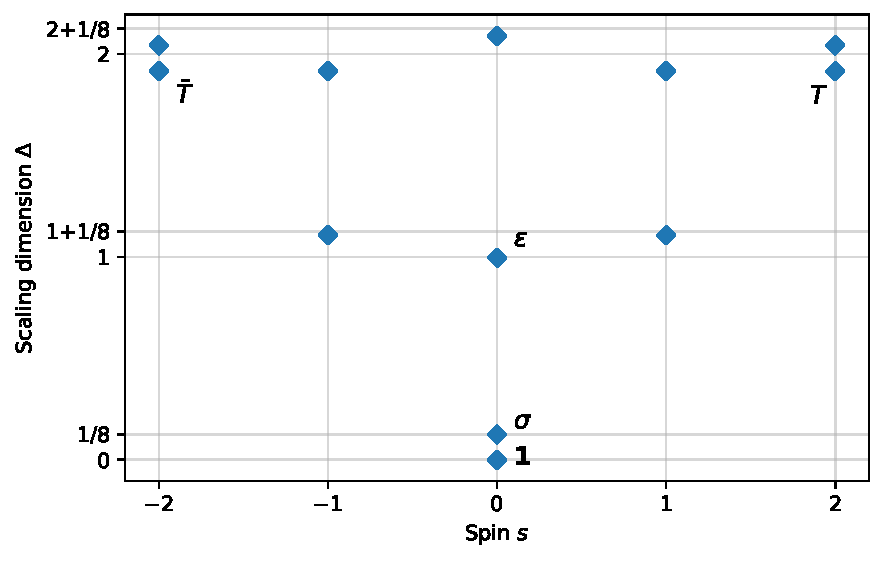
\includegraphics[width=0.7\textwidth]{images/fibonacci/ising-spectrum.pdf}
  \caption[Ising 模型的能谱]{Ising 模型的能谱,对应于 $n\to\infty$ 圆柱转移矩阵。其中初级场及能动量张量使用 CFT 中的相应算符来标记。图片来源:\parencite{zeng2023virasoro}。}
  \label{fig:ising-spectrum}
\end{figure}

除了直接考察能谱数据,我们还可以通过分析能动量张量的两点关联函数来检验其正确性,它们可以使用 iTEBD 算法来计算(见 \ref{subsec:mps-time-evolution} 小节)。首先,我们使用 $A$ 张量来构建一个无限一维链 (iMPS),并将其转化为正则形式。接下来,我们通过对 iMPS 进行虚时演化来计算配分函数。再把 $T$ 插入配分函数中,即可计算得到关联函数,其结果如图~\ref{fig:ising-correlation-functions} 所示。可以发现 $T$ 的两点关联函数存在幂律行为,并且拟合得到的标度维数与表~\ref{tab:ising-spectrum} 中的能谱数据大致相符。

\begin{figure}[ht]
  \centering
  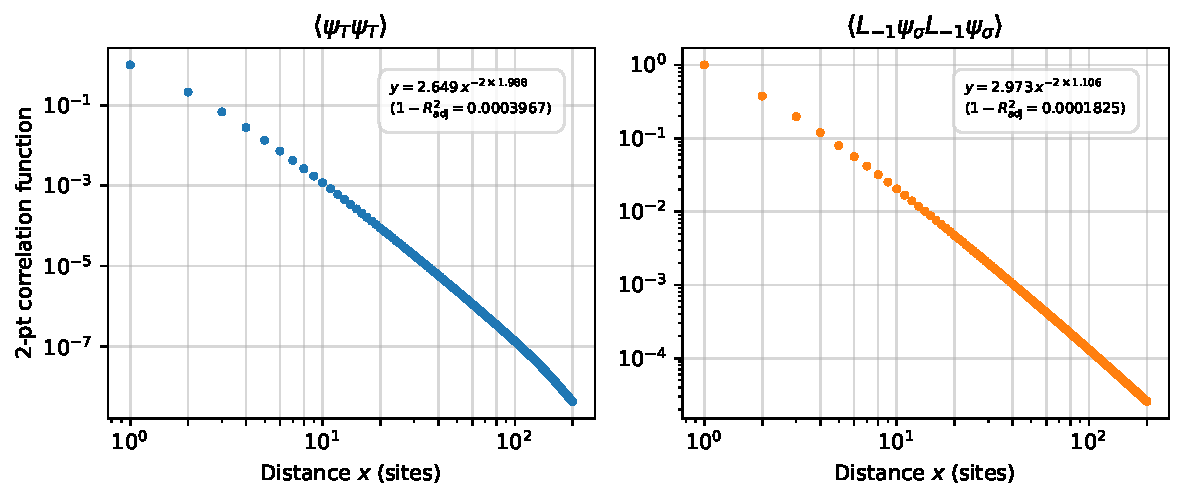
\includegraphics[width=0.9\textwidth]{images/fibonacci/ising-correlation-function.pdf}
  \caption[Ising 模型中的两点关联函数]{Ising 模型中能动量张量 $T$(左图)和 $L_{-1}\phi_\sigma$(右图)的两点关联函数。为了避免计算本征值时有限尺寸效应导致的误差(影响 $x$ 较小的区间),以及 iTEBD 算法中的长程累积误差和 iMPS 本身结构带来的限制(影响 $x$ 较大的区间),我们只取 $x=10$ 到 100 区间的数据来拟合幂律公式 $y=Ax^{-2\Delta}$,此时分别得到 $\Delta=1.988$ 和 1.106。它们与 Ising 能谱的理论结果($\Delta=2$ 和 $1+1/8$)基本相符。图片来源:\parencite{zeng2023virasoro}。}
  \label{fig:ising-correlation-functions}
\end{figure}

\subsection{Virasoro 算符}
\label{subsec:ising-virasoro-operator}

注意到此时 $T$ 和 $\bar{T}$ 的形状和 $A^{(1)}$ 是相同的,我们便可以按照图~\ref{fig:virasoro-construction} 的方法来构造 Virasoro 算符。这里我们仍然选取 $N=8$ 的圆柱,但组成它的张量单元都是经过粗粒近似的 $A^{(1)}$,其连接维数 $\chi=4$。

\begin{figure}[ht]
  \centering
  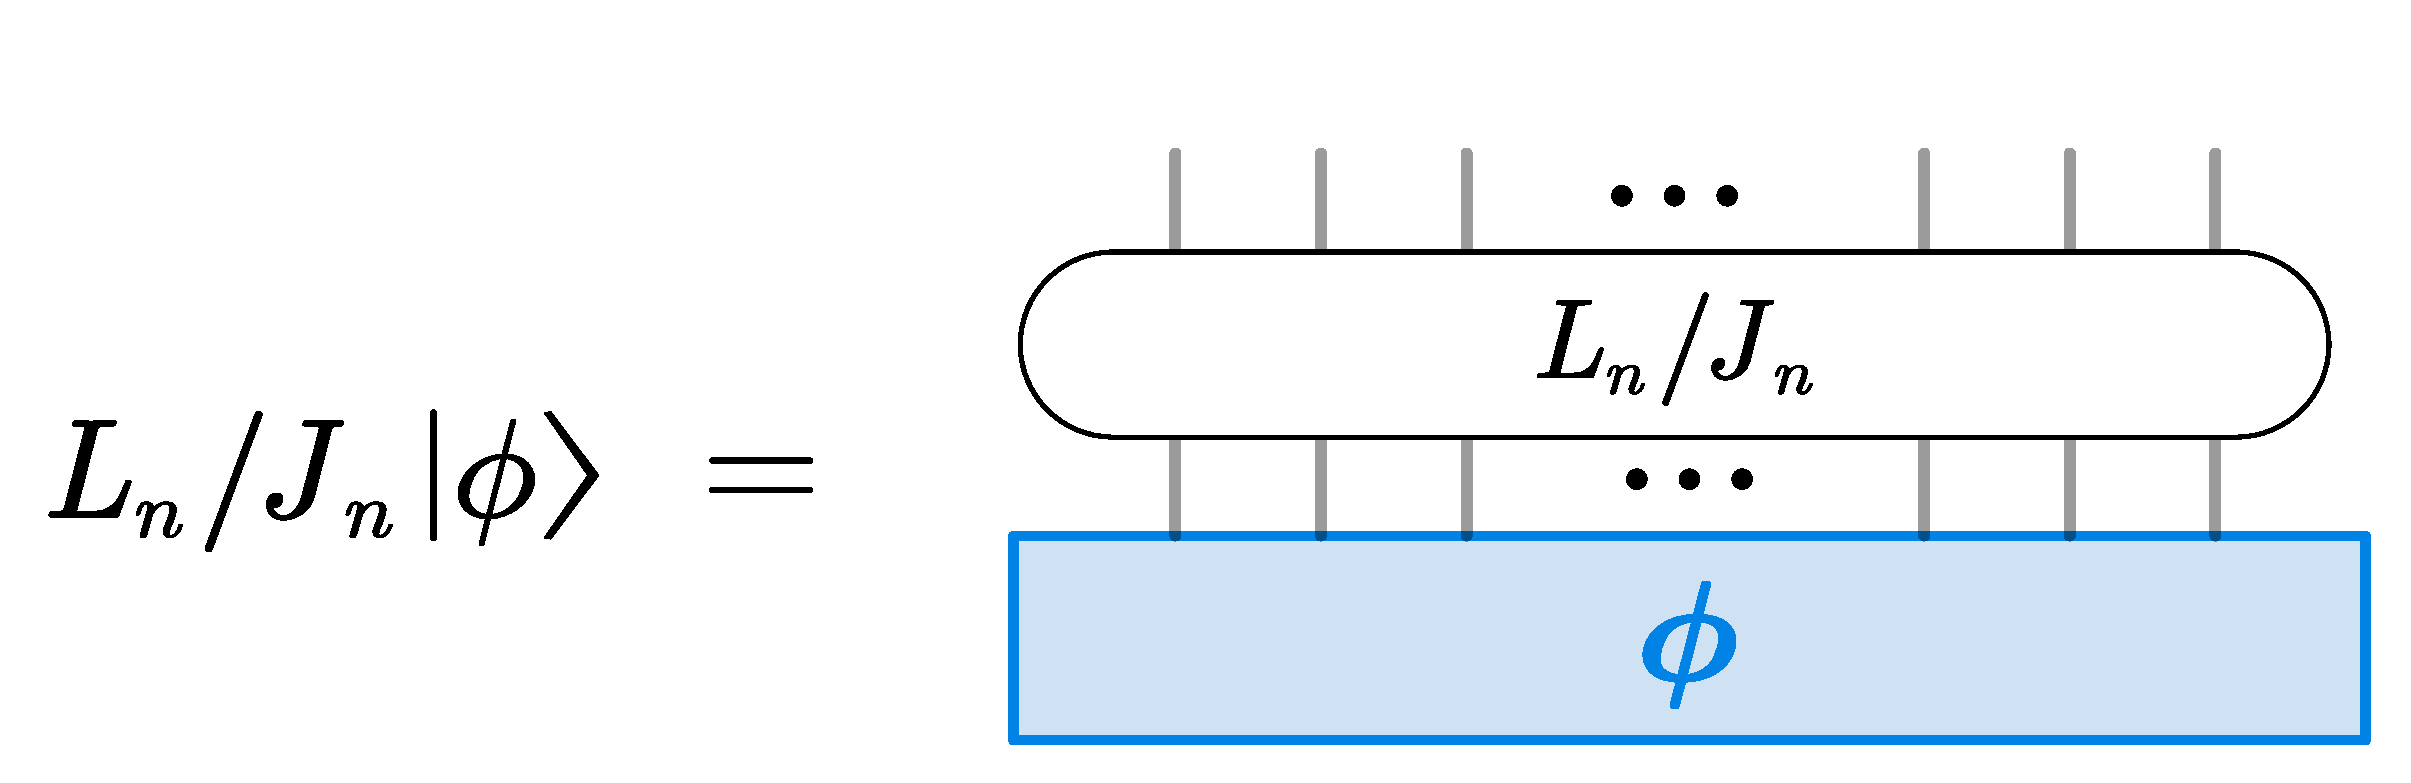
\includegraphics[width=0.5\textwidth]{images/virasoro/operator.pdf}
  \caption[Virasoro 算符作用在本征态上]{Virasoro 算符(或 Kac--Moody 算符)作用在本征态上。图片来源:\parencite{wang2022virasoro}。}
  \label{fig:virasoro-operator}
\end{figure}

为了检验这一方法的正确性,我们把得到的 Virasoro 算符 $L_n$ 和 $\bar{L}_n$ 进一步作用在 $N=8$、$\chi=4$ 圆柱的本征态 $\ket*{\phi_\alpha}$ 上(如图~\ref{fig:virasoro-operator} 所示)。在 CFT 中,Virasoro 算符起到升降算符的作用,使得
\begin{equation}
  L_n         \ket{\Delta_\alpha, s_\alpha} \propto \ket{\Delta_\alpha-n, s_\alpha-n}, \quad
  L_{\bar{n}} \ket{\Delta_\alpha, s_\alpha} \propto \ket{\Delta_\alpha-n, s_\alpha+n}.
\end{equation}
因此只需考察矩阵元 $\langle\phi_\beta|L_n|\phi_\alpha\rangle$ 的值,即可判断 $L_n$ 和 $\bar{L}_n$ 是否能将 $\ket*{\phi_\alpha}$ 映射到相应的态上。我们的计算结果显示,在 Ising 模型中,对于 $N=8$、$\chi=4$ 圆柱的本征态,近似有
\begin{equation}
  \frac{\lVert \langle\phi_\beta|L_n|\phi_\alpha\rangle \rVert}{\lVert \ket*{\phi_\beta} \rVert \cdot \lVert L_n\ket*{\phi_\alpha} \rVert} \gtrsim 0.9, \quad
  n=\pm1, \pm2.
\end{equation}
这说明通过本方法计算得到的格点 Virasoro 算符与 CFT 的理论预言基本是一致的,并且具有比较好的精度。在图~\ref{fig:ising-virasoro} 和 \ref{fig:ising-virasoro-all} 中,我们给出了这些格点 Virasoro 算符作用的示意图。矩阵元的数据可以在文献 \parencite{wang2022virasoro} 的补充材料中找到。我们观察到,在这些矩阵元中,有一些数据的精度相对较低(与正确值相差 1 到 2 个数量级)。造成这种问题的原因主要是格点模型的有限尺寸效应:一方面,在比较小的圆柱中,CFT 的不同本征态实际上是存在交叠的;另一方面,格点 Virasoro 算符也是通过对有限大小的圆柱进行精确对角化求得的,本身也存在一定误差。

Virasoro 算符的正确性同样可以通过两点关联函数来检验。在图~\ref{fig:ising-correlation-functions} 中,我们考察了 $L_{-1}\phi_\sigma$ 的关联函数,拟合得到的标度维数与理论值 $1+1/8$ 也是基本一致的。

\begin{figure}[ht]
  \centering
  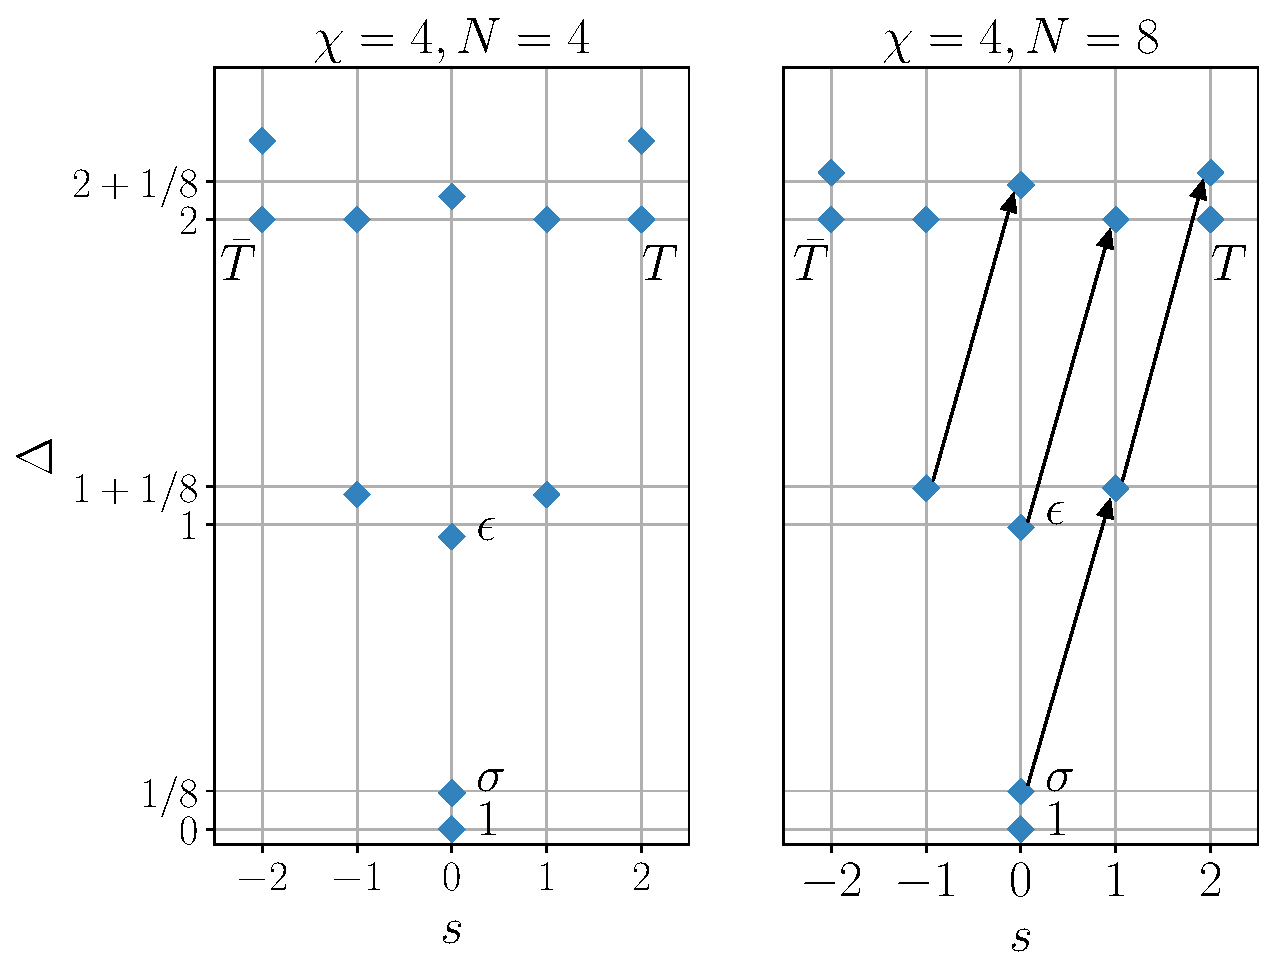
\includegraphics[width=0.7\textwidth]{images/virasoro/ising-spectrum.pdf}
  \caption[Virasoro 算符在 Ising 模型能谱上的作用示意图]{Virasoro 算符 $L_{-1}$ 在 Ising 模型能谱上的作用示意图。能动量张量 $T$ 由 $n=4$、$\chi=4$ 圆柱的本征态得到(左图),由此构造出的 Virasoro 算符 $L_{-1}$ 则作用在 $N=8$、$\chi=4$ 的圆柱上(右图)。更多的例子见图~\ref{fig:ising-virasoro-all}。图片来源:\parencite{wang2022virasoro}。}
  \label{fig:ising-virasoro}
\end{figure}

\section{例子:Dimer 模型}

接下来我们考虑正方形网格上的 dimer 模型\cite{kasteleyn1961statistics,temperley1961dimer,kasteleyn1963dimer}。与 Ising 模型类似,它的配分函数也可以表示为一个二维张量网络,张量单元 $B^{(0)}_{ijkl}$ 中的非零元素为
\begin{equation}
  B^{(0)}_{1111} = B^{(0)}_{2211} = B^{(0)}_{2121} = B^{(0)}_{1212} = B^{(0)}_{2222} = 1, \quad
  B^{(0)}_{1122} = 2.
\end{equation}
在连续极限下,这一模型对应了中心荷 $c=1$ 的自由 Bose 子共形场论\cite{ioffe1989superconductivity,henley1997relaxation,allegra2015exact},其顶点算子 (vertex operator) 具有标度维数和共形自旋
\begin{equation}
  \Delta_{e,m} = e^2 + \frac14 m^2, \quad
  s_{e,m} = em,
\end{equation}
式中 $e$、$m$ 是 dimer 模型 Coulomb 气描述中的电磁荷。

除了 Virasoro 对称性,连续极限下的 dimer 模型还额外具有 Kac--Moody 对称性。由于 Virasoro 生成元的构造方法与 Ising 模型的情况完全一致,这里我们只考察 Kac--Moody 生成元。我们使用 $2\times2$ 个张量单元 $B^{(0)}$ 来构造粗粒近似的张量 $B^{(1)}$,其标度维数 $\chi=4$。对由 $N=4$ 的圆柱(相当于 $N=8$、$\chi=2$ 的圆柱)进行精确对角化可以得到相应的能谱数据,而 $\ket*{\phi_J}$ 和 $\ket*{\phi_{\bar{J}}}$ 就分别对应了 $s=\pm1$ 的两个最低能级。将其变形后可以得到 4 个指标、$\chi=4$ 的张量 $J$ 和 $\bar{J}$,即流算符的近似格点表示。

\begin{figure}[ht]
  \centering
  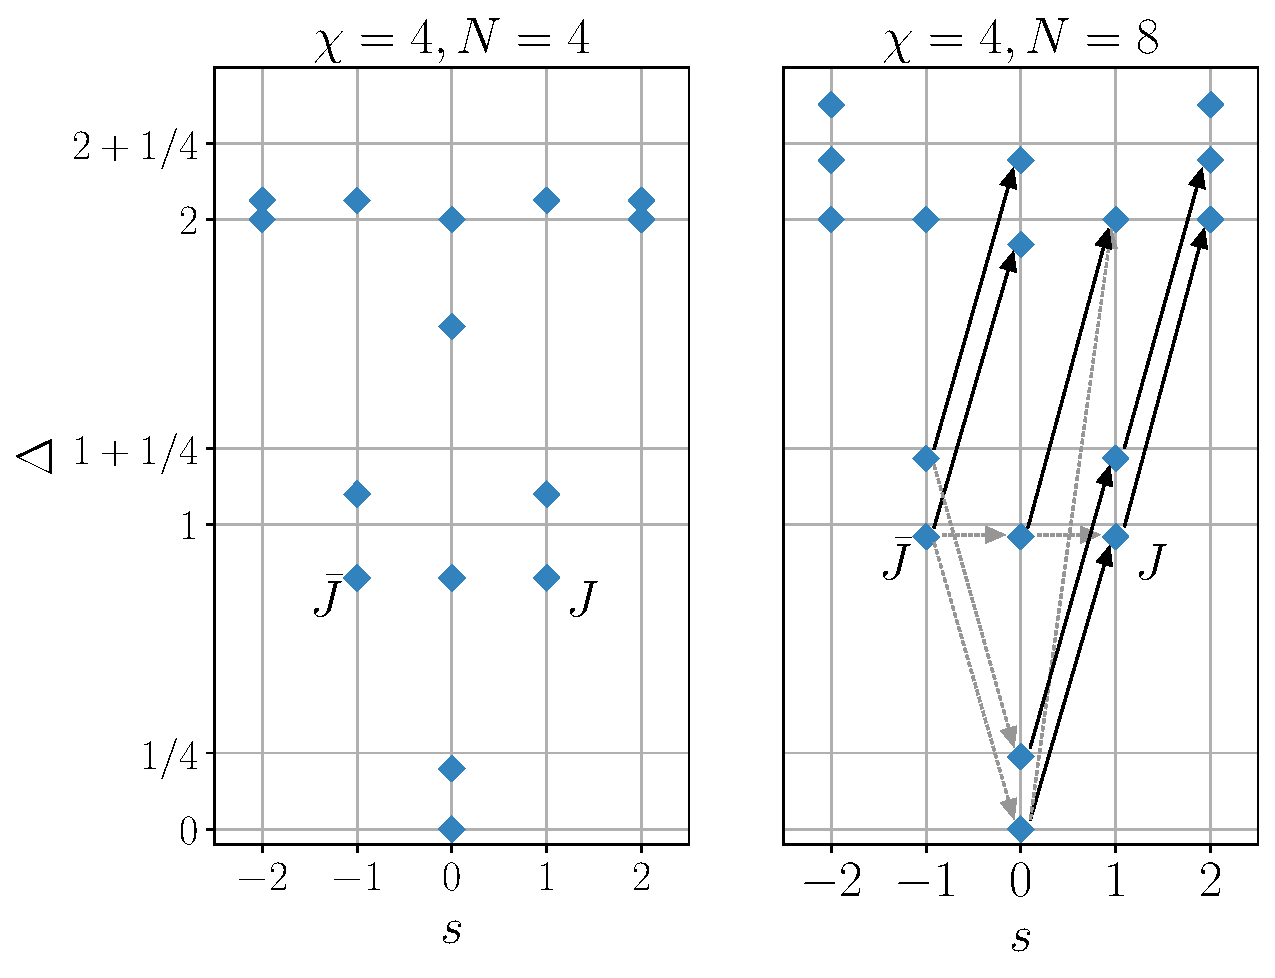
\includegraphics[width=0.7\textwidth]{images/virasoro/dimer-spectrum.pdf}
  \caption[Kac--Moody 算符在 dimer 模型能谱上的作用示意图]{Kac--Moody 算符 $J_{-1}$ 在 dimer 模型能谱上的作用示意图。近似的流算符 $J$ 由 $n=4$、$\chi=4$ 圆柱的本征态得到(左图),由此构造出的 Kac--Moody 算符 $J_{-1}$ 则作用在 $N=8$、$\chi=4$ 的圆柱上(右图)。其中,符合 CFT 预测的作用使用黑色实线箭头标记,而不相符的则用灰色虚线箭头标记。更多的例子见图~\ref{fig:dimer-kac-moody-all}。图片来源:\parencite{wang2022virasoro}。}
  \label{fig:dimer-kac-moody}
\end{figure}

同样按照图~\ref{fig:virasoro-construction} 和 \ref{fig:virasoro-operator} 中的方法,我们选取 $N=8$、$\chi=4$ 的圆柱来构造并检验 Kac--Moody 生成元。Kac--Moody 算符满足
\begin{equation}
  J_n         \ket{\Delta_\alpha, s_\alpha} \propto \ket{\Delta_\alpha-n, s_\alpha-n}, \quad
  J_{\bar{n}} \ket{\Delta_\alpha, s_\alpha} \propto \ket{\Delta_\alpha-n, s_\alpha+n}.
\end{equation}
因此通过考察矩阵元 $\langle\phi_\beta|J_n|\phi_\alpha\rangle$ 即可判断 $J_n$ 和 $\bar{J}_n$ 是否能正确起到升降算符的作用。计算结果表明,对于初始态 $\ket{\phi_\alpha}=\ket{\Delta_\alpha,s_\alpha}$,按上述方法构造出的格点 Kac--Moody 算符能够将其映射到正确的后代 $\ket{\phi_\beta}=\ket{\Delta_\beta,s_\beta}$ 上。然而,在这些矩阵元中我们也观察到了一些错误值。相比于 Ising 的情况,dimer 模型中有更严重的限尺寸效应,因而误差也更加显著。这些错误值主要有以下两类:

\begin{itemize}
  \item 不同 Kac--Moody 后代之间的混淆(主要是 $\ket{s=0,\Delta=0}$ 和 $\ket{s=0,\Delta=1}$ 的后代之间),这可能是由于圆柱的最低本征态并非真实的真空态,而是包含了其他初级场的污染;
  \item 同一组 Kac--Moody 后代中升/降作用的混淆,这表明格点流算符的全纯与反全纯部分很可能没有完全分离。
\end{itemize}

需要指出的是,这些矩阵元之间的混淆具有一些特定的模式(见文献 \parencite{wang2022virasoro} 补充材料中的数据),这说明计算所得的基态是真实的真空态与一些较低能级简并态的混合,而且混合关系是固定的。此外我们还可以观察到,相比那些不能通过 Kac--Moody 代数从某些初级场生成的能级,矩阵元之间的差异仍有 5--6 个数量级。因而这表明我们的构造方案仍染有效,并且原则上也可以将这些本征态分离开来(可能需要使用更大的圆柱以减小有限尺寸效应的影响)。

\section{例子:Fibonacci 模型}

在很大程度上,Ising 模型具有一定的特殊性,例如它受有限尺寸效应的影响较小。对于更一般的模型,无论是计算与确定圆柱本征态,还是构造对应的 Virasoro 算符,都较为困难。本小节我们将考察 $\mathbb{Z}_3$ parafermion CFT,它可以通过为 Fibonacci 弦网模型添加适当的边界条件而得到。

\subsection{转移矩阵}

Fibonacci 弦网模型定义在六边形网格上,包含 $\1$ 和 $\tau$ 两种简单对象,对应的三角形和正方形张量单元已经分别在 \ref{subsec:strange-correlator-fib} 和 \ref{subsec:central-charge} 小节中给出:
\begin{gather}
    \Triangle \tau\tau\tau\tau\tau\tau
  = \varphi^{\frac14} \bigl[ F^{\tau\tau\tau}_\tau \bigr]_{\tau\tau} = -\varphi^{-\frac34}, \quad
    \Triangle \tau\tau\tau\1\tau\tau
  = \varphi^{\frac{7}{12}} \bigl[ F^{\tau\tau\tau}_\tau \bigr]_{\tau\1} = \varphi^{\frac{1}{12}};
  \label{eq:fib-triangles} \\
    A_{ijkl} = \tikzinput{fibonacci/square-1} = \tikzinput{fibonacci/square-2}.
  \label{eq:fib-square}
\end{gather}
同样,转移矩阵也是由张量单元 $A$ 构成的:
\begin{equation}
    \tilde{M}_{i_1 i_2 \cdots i_n, \, j_1 j_2 \cdots j_n}
  = \sum_{\substack{i_1, i_2, \ldots, i_n \\ j_1, j_2, \ldots, j_n}}
    \prod_{\alpha=1}^n A_{i_\alpha j_\alpha j_{\alpha+1} i_{\alpha+1}}
  = \tikzinput{fibonacci/cylinder} \, .
\end{equation}
但与正方形网格(如二维 Ising 模型)的情况不同,这里 $A_{ijkl}$ 的指标位于四个角,所以在缩并时需要仔细处理各指标的顺序。此外,上述圆柱 $\tilde{M}$ 并不是 Hermitian 的,因此并不能直接构成正确的转移矩阵。如果把 这些圆柱堆叠起来,在最终计算得到的能谱中将会出现额外的相位。我们可以把两个方向相反的圆柱叠加起来,即选取
\begin{equation}
  M = \tilde{M}\tilde{M}^\dagger,
\end{equation}
这时就可以消除相位的影响,得到正确的转移矩阵。

\subsection{CFT 能谱与能动量张量}

在热力学极限下,Fibonacci 弦网模型(也即中心荷 $c=4/5$ 的 hard-hexagon 模型)将会收敛到 $\mathbb{Z}_3$ parafermion CFT,但并非所有的拓扑缺陷在格点近似中都存在对应的矩阵乘积算符 (MPO) 表示\cite{vanhove2018mapping}。我们并不需要考虑拓扑缺陷,而这种“空”的环面配分函数可以通过取大小为 $n=3k$ 的圆柱得到。相应地,平移算符也需要改为使用把格点平移 3 个单位的 $P^3$。

随着圆柱尺寸 $n$ 的增加,计算中内存消耗是指数级增长的。为了能够处理较大的圆柱,我们这里采用了矩阵无关 (matrix-free) 的线性算符 (linear operator) 方法,即不再显式地构造转移矩阵 $M$,而是计算 $M$ 作用在某个向量上的结果。如图~\ref{fig:fib-linear-operator} 所示,由于 $M$ 是通过张量单元 $A_{ijkl}$ 构造而成的,矩阵乘法 $M\cdot v$ 可利用多次张量缩并来实现。而平移算符则可以通过对数组元素的重新排列来获得。对于大小为 $n$ 的圆柱,线性算符方法可将内存消耗由 $\mathcal{O}(\chi^{2n})$ 降低到 $\mathcal{O}(\chi^n)$。对于 Fibonacci 模型的情况,在典型配置的服务器上最大可以计算到约 $n\simeq30$ 的情形。

\begin{figure}[ht]
  \tikzinput{fibonacci/linear-operator}
  \caption[利用线性算符方法实现矩阵乘法]{对于 Fibonacci 弦网模型,利用线性算符方法实现矩阵乘法 $M\cdot v$。图片来源:\parencite{zeng2023virasoro}。}
  \label{fig:fib-linear-operator}
\end{figure}

计算得到的能谱数据列在表~\ref{tab:fib-spectrum} 中。由于 Fibonacci 模型中有限尺寸效应较为显著,只有 $n\gtrsim20$ 的圆柱本征值才能给出相对准确的结果。对于较小的圆柱体,一些激发态可能甚至不会出现在能谱中。原则上,将计算结果与标度维数和自旋的理论值进行对比,即可确定对应能级的本征态,例如能动量张量对应的 $\ket*{\phi_T}$。但由于有限尺寸效应,不仅本征值与其理论结果相差甚远,而且还普遍存在能级交错的现象——当圆柱较小时,某些在热力学极限下本应位于较高激发态的能级反而会拥有较小的本征值,这样就很难与其他能级区分开来。

为了在有限尺寸下也能区分不同的本征态,首先我们假设标度维数 $\Delta$ 将大致按照
\begin{equation}
  \Delta = A + \frac{B}{n}
\end{equation}
的形式趋近于其热力学极限值\cite{schuler2016universal},然后我们在能谱中选择相应的数据以使拟合结果最优(即挑选出最接近拟合曲线的数据点,见图~\ref{fig:fib-fitting})。计算出拟合参数 $A$ 后,令 $n\to\infty$ 即可得到 $\Delta^\infty$。这些数据列在表~\ref{tab:fib-spectrum} 的“$\infty$”栏中。进一步,我们还根据式~\eqref{eq:scaling-dimension-rescale} 标定了能谱中的本征值,使得 $\Delta_{\1}=0$、$\Delta_T=2$,从而可以更为准确地估计标度维数。这些数据列在了“调整值”一栏,并且绘制在了图~\ref{fig:fib-spectrum} 中。

\begin{figure}[ht]
  \centering
  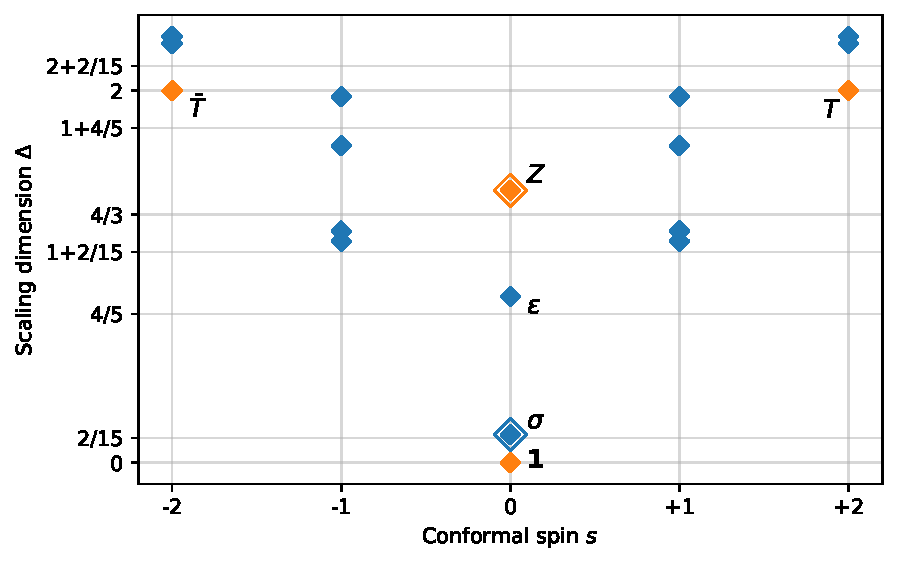
\includegraphics[width=0.7\textwidth]{images/fibonacci/fib-spectrum.pdf}
  \caption[Fibonacci 模型的能谱]{Fibonacci 模型的能谱,对应于 $n\to\infty$ 圆柱转移矩阵。“\tikzinput{fibonacci/spectrum-label}\unskip”表明存在二重简并。图中的本征值进行了缩放处理,以使得 $\Delta_{\1}=0$ 和 $\Delta_T=2$。初级场使用对应的算符来标记,它们的共形维数分别为 $h_{\1}=0$,$h_\sigma=1/15$,$h_\epsilon=2/5$,$h_Z=2/3$,$h_X=7/5$ 以及 $h_Y=3$(与 $X$、$Y$ 对应的态本征值较大,在我们的计算中没有考虑)。CFT 配分函数为 $Z=|\chi_{\1}+\chi_Y|^2+|\chi_\epsilon+\chi_X|^2+2|\chi_\sigma|^2\discretionary{}{}{}+2|\chi_Z|^2$\cite{vanhove2018mapping}。对应于 $|\chi_{\1}+\chi_Y|^2$ 的子空间,其中的本征态用橙色标记。图片来源:\parencite{zeng2023virasoro}。}
  \label{fig:fib-spectrum}
\end{figure}

在拟合中还可以考虑高阶修正项,如
\begin{equation}
  \Delta = A + \frac{B}{n} + \frac{C}{n^2},
\end{equation}
其拟合结果在图~\ref{fig:fib-fitting} 中用虚线标出。高阶项可以给出更好的拟合结果,但由于我们只需要通过这一方法来确定 CFT 中的各能级,因此只需考虑一阶修正项。

\begin{figure}[ht]
  \centering
  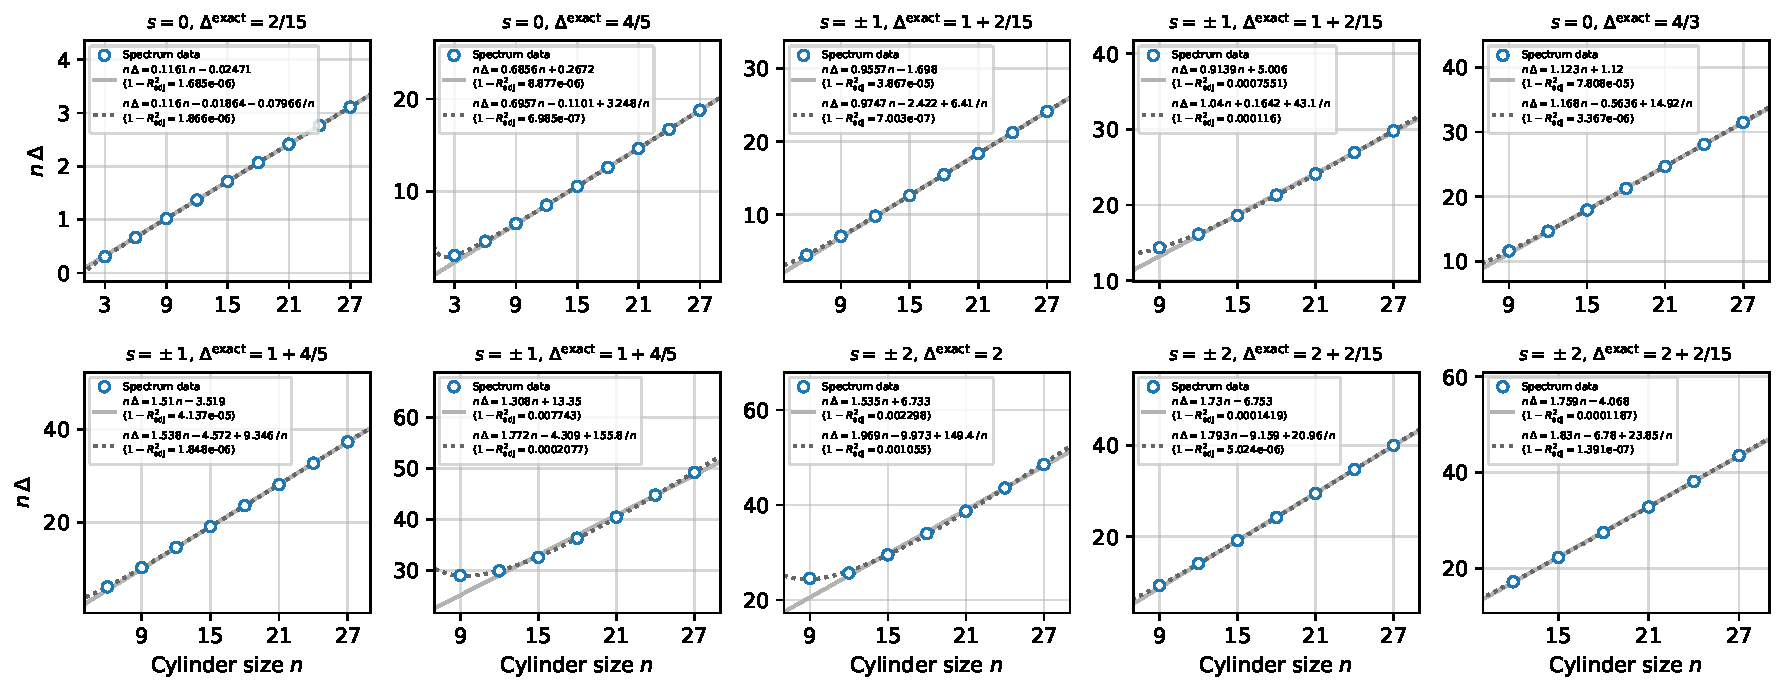
\includegraphics[width=\textwidth]{images/fibonacci/fib-fitting.pdf}
  \caption[Fibonacci 能谱的拟合结果]{Fibonacci 能谱的拟合结果。在拟合 $n\Delta=An+B$ 时,我们仅使用了 $n=12$ 到 27 的圆柱(实线);而在拟合 $n\Delta=An+B+C/n$ 时,我们使用了所有可用的 $n$(虚线)。图片来源:\parencite{zeng2023virasoro}。}
  \label{fig:fib-fitting}
\end{figure}

\subsection{拓扑投影算符}
\label{subsec:topological-projectors}

然而,当太多能级混杂在一起时,上述的拟合方法也无法保证能够将各能级区分开来。例如,当两个能级的自旋相同、标度维数又很接近时,仅从拟合优度并不能分辨。为此,我们需要利用\emph{拓扑投影算符} (topological projectors)\cite{bultinck2017anyons,williamson2017symmetry,aasen2020topological},它可以将转移矩阵投影到对应于特定拓扑荷 (topological charge) 的子空间。拓扑荷与格点模型的尺寸是无关的,因此在热力学极限下趋于能动量张量的本征态,即使在有限大小的系统中也仍然会保持在同一个分区 (sector) ,即包含了真空态的平凡分区。它们在特定的投影算符作用之下可以保留在能谱中,而其他态则会被移除(即投影到零值)。

拓扑投影算符的构造与 \emph{Ocneanu 管状代数} (Ocneanu's tube algebra)\cite{evans1995ocneanu,evans1998quantum}有关(见 \ref{subsec:tube-algebra-idempotents} 小节)。拓扑序模型中的每种任意子都对应着 CFT 中的一个拓扑分区,换而言之 CFT 中的初级场及其后代组成的“家族” (family) 可按照对应的任意子类型进行分类。拓扑序中的弦算符则可作为投影算符,将转移矩阵投影到包含相应拓扑分区的子空间上。因为我们这里的工作主要关注能动量张量,而能动量张量与真空态属于同一分区,所以只需构造与任意子 $\1$ 相对应的弦算符。

在张量网络的语言中,弦算符的一般形式可由 MPO 来描述,称为\emph{中心幂等元} (central idempotent)\cite{bultinck2017anyons,williamson2017symmetry,vanhove2018mapping,lootens2019cardy,aasen2020topological}。构成这些 MPO 的矩阵单元为
\begin{equation}
  \begin{aligned}
       \tikzinput{idempotents-mpo-1}
    &= (d_\alpha d_\beta d_\gamma d_\delta)^{\frac14} G^{\beta i\gamma}_{j\alpha\delta}, \\
       \tikzinput{idempotents-mpo-2}
    &= (d_\alpha d_\beta d_\gamma d_\delta d_i d_j d_k)^{\frac14}
       G^{k\beta\delta}_{ij\alpha} G^{i\gamma\beta}_{kj\delta},
  \end{aligned}
\end{equation}
其中 $G$ 可通过对四面体张量($F$ 符号)进行归一化和对称化得到:
\begin{equation}
    G^{abc}_{ijk}
  = \frac{1}{\sqrt{d_j d_c}} \bigl[ F^{aik}_b \bigr]_{jc}
  = \frac{1}{\sqrt{d_a d_b d_c d_i d_j d_k}} \, \Tetrahedron jibcka.
\end{equation}
对于大小为 $n$ 的圆柱转移矩阵,管状代数的基\footnote{在中心幂等元的构造中,\ref{subsec:tube-algebra-idempotents} 小节中带有 4 个指标的 $\mathcal{T}^{s}_{pqr}$ 需要满足 $r=p$,因此这里的 $\mathcal{T}^{c}_{ab}\coloneq\mathcal{T}^{c}_{bab}$。}可由 $n-1$ 个橙色张量与一个红色张量首尾相连得到:
\begin{equation}
  \mathcal{T}^{c}_{ab} = \tikzinput{tube-algebra-basis}.
\end{equation}
注意图中省略了辅助指标,它们需要被正常缩并掉。

中心幂等元的一般形式可表示为这些基的线性组合。在式~\eqref{eq:fib-idempotents} 中,我们已经给出了 Fibonacci 模型中对应于 $\1$ 的中心幂等元:
\begin{equation}
  \mathcal{P}_{1} = \frac{1}{\sqrt5}
  \left( \frac{1}{\phi} \mathcal{T}^{\1}_{\1\1} + \sqrt{\phi} \mathcal{T}^{\tau}_{\tau\1} \right).
\end{equation}
它可以与转移矩阵、平移算符相连,再进行对角化便可得到只含真空态、能动量张量等的子能谱。这样,即使是在有限尺寸下,依然可以严格地找到能动量张量对应的本征态。我们在表~\ref{tab:fib-spectrum} 和图~\ref{fig:fib-spectrum} 中都对这些态做了高亮。

\subsection{Virasoro 算符}

接下来我们按照 \ref{sec:virasoro-operators} 节中介绍的方法来构造 Virasoro 算符。考虑到 Fibonacci 模型要求圆柱大小 $n=3k$,此时由对角化求得的能动量张量 $T$ 和 $\bar{T}$ 并不能像 Ising 模型的情况一样直接插回圆柱。因此,我们需要首先把 $T$ 和 $\bar{T}$ 变形为三角形,再用式~\eqref{eq:fib-triangles} 中的三角形张量单元补成正方形,这与式~\eqref{eq:fib-square} 是类似的:
\begin{equation}
  \tikzinput{fibonacci/padded-tensor-1} = \tikzinput{fibonacci/padded-tensor-2} \to \tikzinput{fibonacci/padded-tensor-3}.
\end{equation}
注意在缩并时只有角上的自由度需要考虑。圆柱中的其他张量也可以用类似的方式构造,但方便起见,也可以等价地用 $k\times k$ 个式~\eqref{eq:fib-square} 中的正方形缩并得到。

计算中我们用 $n=18$ 的圆柱来计算本征态,并得到对应的能动量张量。之后,将其变形并补全成正方形张量,此时连接维数 $\chi=2^{n/3}$。我们同样按照图~\ref{fig:virasoro-construction} 的方式构造 Virasoro 算符。尽管原则上圆柱的大小 $N$ 可以取任意值,但由于内存的限制,这里最大只能取到 $N=3$。检验 Virasoro 算符正确性的方法与 \ref{subsec:ising-virasoro-operator} 小节相同,也是检查 $L_n$ 和 $\bar{L}_n$ 是否能将圆柱本征态 $\ket*{\phi_\alpha}$ 正确地升高或降低到对应能级。在图~\ref{fig:fib-virasoro} 和 \ref{fig:fib-virasoro-all} 中,我们给出了这些格点 Virasoro 算符作用的示意图。矩阵元的数据则可在文献 \parencite{zeng2023virasoro} 的补充材料中找到。

\begin{figure}[ht]
  \centering
  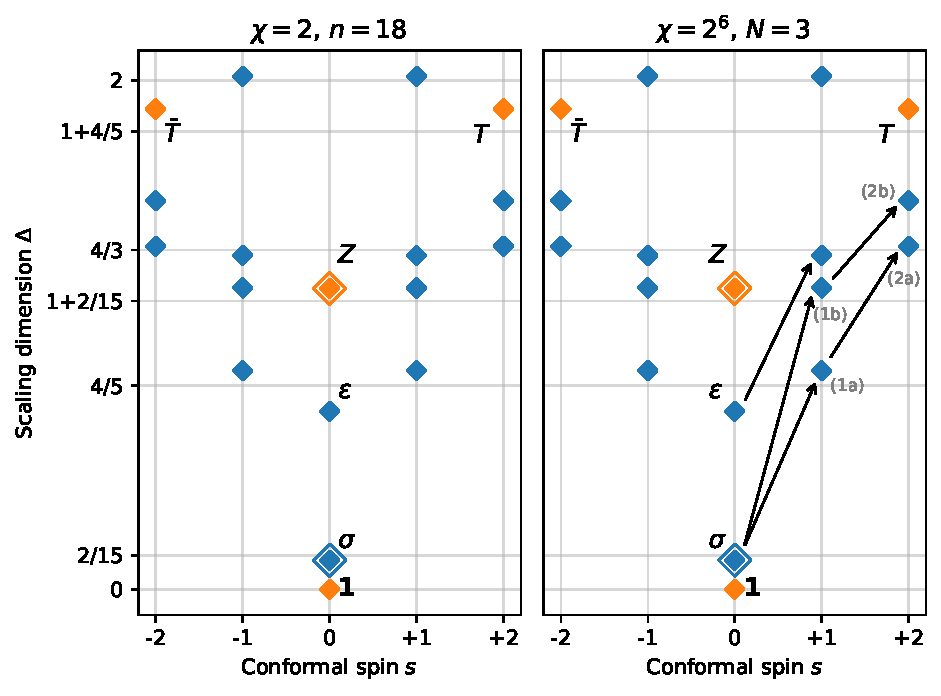
\includegraphics[width=0.7\textwidth]{images/fibonacci/fib-virasoro.pdf}
  \caption[Virasoro 算符在 Fibonacci 模型能谱上的作用示意图]{Virasoro 算符 $L_{-1}$ 在 Fibonacci 模型能谱上的作用示意图。能动量张量 $T$ 由 $n=18$、$\chi=2$ 圆柱的本征态得到(左图),由此构造出的 Virasoro 算符 $L_{-1}$ 则作用在 $N=3$、$\chi=2^{n/3}$ 的圆柱上(右图)。标记为 (1a)\,/\,(1b) 和 (2a)\,/\,(2b) 的两组本征态在 CFT 极限下应当是简并的,但由于有限尺寸效应,它们的标度维数并不相同(可对比图~\ref{fig:fib-spectrum})。更多的例子见图~\ref{fig:fib-virasoro-all}。图片来源:\parencite{zeng2023virasoro}。}
  \label{fig:fib-virasoro}
\end{figure}

\section{本章小结}

本章首先回顾了二维共形场论的基本概念,尤其是 Virasoro 与 Kac--Moody 代数。在二维格点模型配分函数的张量网络表示中,我们给出了通过能动量张量或流算符来构造 Virasoro 与 Kac--Moody 算符的方法。具体来说,我们将积分用一个新的圆柱形张量网络来表示,并把能动量张量(或流算符)插入其中。由此得到的 Virasoro 和 Kac--Moody 生成元可以作用在任意的本征态上,进而可以用来检验这一方法的有效性。在 Ising 和 dimer 模型中的数值结果则表明,即使是在较小的系统中,利用这套方案构造出的 Virasoro 与 Kac--Moody 算符也能达到很高的精度。而在受有限尺寸效应影响较大的系统(如 Fibonacci 模型)中,即使采用尺寸较大的圆柱,也很难从中得到准确的 CFT 能谱等数据。为此,我们首先对不同大小的圆柱进行精确对角化,并根据拟合结果来区分不同的本征态;对于混淆较为严重的态,我们还引入了拓扑投影算符,将转移矩阵投影到对应于特定拓扑荷的子空间中,这样也构造出了符合预期精度的 Virasoro 算符。

\chapter{全息张量网络中的重整化群}


\backmatter

\bibliography{main}

\end{document}
